\subsection{Parametry kamene \textit{viva12}}

Šatonová růže má 14 rovinných faset. Fasety označujeme zkratkami \textbf{TOP}, \textbf{BOT} a \textbf{UF1-UF12}, kde

\begin{tabular}{l l}
\textbf{TOP} & - tabulka,\\
\textbf{BOT} & - spodek,\\
\textbf{UF1-UF12} & - 12 bočních faset.\\
\end{tabular}\\

Označené fasety máme na obrázku \ref{fig:viva12Params} spolu s vyznačenými parametry

\begin{tabular}{l l}
$d_{TOP}$ & průměr tabulky,\\
$d_{BOT}$ & průměr spodku,\\
$h$ & výška kamene,\\
$h_{RF}$ & výška lemu. 
\end{tabular}\\
 
Poznamenejme, že lem modelujeme množstvím faset, které po spojení aproximují oválný tvar. Tyto fasety mají v simulaci absorpční charakter. Světelné svazky, které na ně dopadnou, zaniknou.   

\begin{figure}[htps]
\centering
\begin{minipage}[c]{0.4\textwidth}
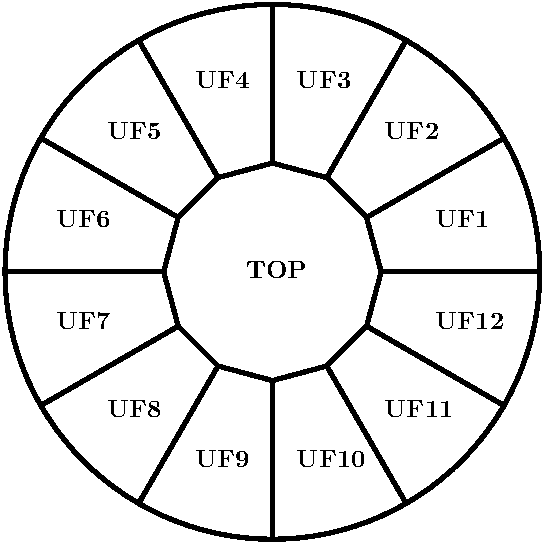
\includegraphics[width=\textwidth]{vivi12Facets1.pdf}
\end{minipage}
\begin{minipage}[c]{0.56\textwidth}
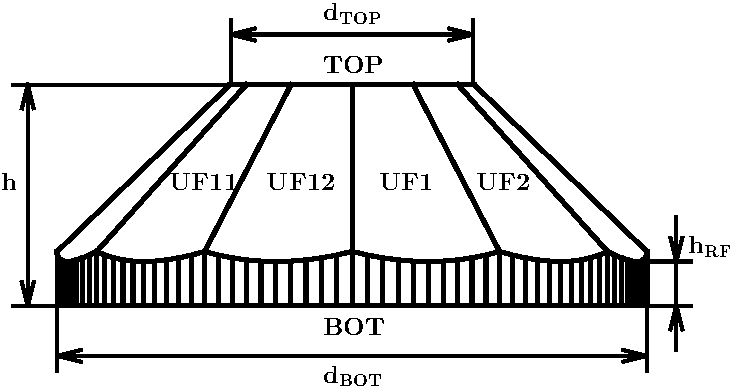
\includegraphics[width=\textwidth]{vivi12Facets2.pdf}
\end{minipage}
\caption{Šatonová růže s označenými fasetami a parametry. Pohled shora je zobrazen vlevo, bokorys vpravo.}
\label{fig:viva12Params}
\end{figure}

\subsection{Klasifikace svazků do tříd}
Typ svazku definujeme podle pořadí dopadových faset. Při opakovaném použití ovšem tento způsob popisu není přehledný.

 Pro lepší orientaci si svazky rozdělíme do tříd a budeme pracovat pouze s jejím názvem. Název je u všech tříd dvouciferný.
 
  První cifra udává počet dopadových faset. Zde se pohybujeme od 1 do 9. Svazky s větším počtem dopadových faset než 9 nejsme schopni na stínítku rozpoznat a definovat je nemá smysl. 
  
  Na pozici druhé cifry se objevují znaky abecedy \textit{A-Z}. Svazky s jednotným počtem odrazů se začínají značit od písmene \textit{A} a to tak, že \textit{A} patří třídě svazků, která má největší zářivý tok. Zářivý tok třídy svazků postupně klesá s abecedním pořadím. Svazky, které nemají dostatečný zářivý tok a nelze je spařit na stínítku neuvádíme. 
  
  Svazky popisujeme pro situaci, kdy směrový vektor zdrojového svazku je přibližně kolmý k rovině spodku. Pokud bychom kámen orientovali jinak, řada tříd by přestala existovat a zároveň by se objevily i nové nepopsané třídy. 
  
  Rozdělení svazků do tříd je zapsáno v tabulkách \ref{table:TableClasses1}, \ref{table:TableClasses2}, \ref{table:TableClasses3}, \ref{table:TableClasses4}, \ref{table:TableClasses5} a \ref{table:TableClasses6}.
  
  
 
 
  


\begin{table}[h!]
\centering
\begin{tabular}{|l|c|c|c|c|c|c|c|c|c|c|c|c|}
\hline
Class &  \multicolumn{9}{l}{Ray path} \vline  & Count\\
\hline \hline
\textbf{1A} & UF1 & UF2 & UF3 & UF4 & UF5 & UF6 & UF7 & UF8 & $\dots$ & 12\\
\hline \hline
\textbf{1B} & \multicolumn{9}{l}{TOP} \vline  & 1\\
\hline \hline
\textbf{3A} & UF1 & UF2 & UF3 & UF4 & UF5 & UF6 & UF7 & UF8 & $\dots$ & 12\\
 & BOT & BOT & BOT & BOT & BOT & BOT & BOT & BOT & $\dots$ & \\
 & TOP & TOP & TOP & TOP & TOP & TOP & TOP & TOP & $\dots$ & \\
\hline \hline
\textbf{3B} & \multicolumn{9}{l}{TOP-BOT-TOP} \vline  & 1\\
\hline \hline
\textbf{5A} & UF1 & UF2 & UF3 & UF4 & UF5 & UF6 & UF7 & UF8 & $\dots$ & 12\\
 & BOT & BOT & BOT & BOT & BOT & BOT & BOT & BOT & $\dots$ & \\
 & TOP & TOP & TOP & TOP & TOP & TOP & TOP & TOP & $\dots$ & \\
 & BOT & BOT & BOT & BOT & BOT & BOT & BOT & BOT & $\dots$ & \\
 & UF6 & UF7 & UF8 & UF9 & UF10 & UF11 & UF12 & UF1 & $\dots$ & \\
\hline \hline
\textbf{5B} & UF1 & UF2 & UF3 & UF4 & UF5 & UF6 & UF7 & UF8 & $\dots$ & 12\\
 & BOT & BOT & BOT & BOT & BOT & BOT & BOT & BOT & $\dots$ & \\
 & TOP & TOP & TOP & TOP & TOP & TOP & TOP & TOP & $\dots$ & \\
 & BOT & BOT & BOT & BOT & BOT & BOT & BOT & BOT & $\dots$ & \\
 & UF7 & UF8 & UF9 & UF10 & UF11 & UF12 & UF1 & UF2 & $\dots$ & \\
\hline \hline
\textbf{5C} & UF1 & UF2 & UF3 & UF4 & UF5 & UF6 & UF7 & UF8 & $\dots$ & 12\\
 & BOT & BOT & BOT & BOT & BOT & BOT & BOT & BOT & $\dots$ & \\
 & TOP & TOP & TOP & TOP & TOP & TOP & TOP & TOP & $\dots$ & \\
 & BOT & BOT & BOT & BOT & BOT & BOT & BOT & BOT & $\dots$ & \\
 & UF8 & UF9 & UF10 & UF11 & UF12 & UF1 & UF2 & UF3 & $\dots$ & \\
\hline \hline
\textbf{5D} & UF1 & UF2 & UF3 & UF4 & UF5 & UF6 & UF7 & UF8 & $\dots$ & 12\\
 & BOT & BOT & BOT & BOT & BOT & BOT & BOT & BOT & $\dots$ & \\
 & TOP & TOP & TOP & TOP & TOP & TOP & TOP & TOP & $\dots$ & \\
 & BOT & BOT & BOT & BOT & BOT & BOT & BOT & BOT & $\dots$ & \\
 & TOP & TOP & TOP & TOP & TOP & TOP & TOP & TOP & $\dots$ & \\
\hline \hline
\textbf{5E} & \multicolumn{9}{l}{TOP-BOT-TOP-BOT-TOP} \vline  & 1\\
\hline \hline
\textbf{6A} & UF1 & UF2 & UF3 & UF4 & UF5 & UF6 & UF7 & UF8 & $\dots$ & 12\\
 & BOT & BOT & BOT & BOT & BOT & BOT & BOT & BOT & $\dots$ & \\
 & UF1 & UF2 & UF3 & UF4 & UF5 & UF6 & UF7 & UF8 & $\dots$ & \\
 & UF6 & UF7 & UF8 & UF9 & UF10 & UF11 & UF12 & UF1 & $\dots$ & \\
 & BOT & BOT & BOT & BOT & BOT & BOT & BOT & BOT & $\dots$ & \\
 & UF8 & UF9 & UF10 & UF11 & UF12 & UF1 & UF2 & UF3 & $\dots$ & \\
\hline \hline
\textbf{6B} & UF1 & UF2 & UF3 & UF4 & UF5 & UF6 & UF7 & UF8 & $\dots$ & 12\\
 & BOT & BOT & BOT & BOT & BOT & BOT & BOT & BOT & $\dots$ & \\
 & UF12 & UF1 & UF2 & UF3 & UF4 & UF5 & UF6 & UF7 & $\dots$ & \\
 & UF6 & UF7 & UF8 & UF9 & UF10 & UF11 & UF12 & UF1 & $\dots$ & \\
 & BOT & BOT & BOT & BOT & BOT & BOT & BOT & BOT & $\dots$ & \\
 & UF7 & UF8 & UF9 & UF10 & UF11 & UF12 & UF1 & UF2 & $\dots$ & \\
\hline \hline
\textbf{6C} & UF1 & UF2 & UF3 & UF4 & UF5 & UF6 & UF7 & UF8 & $\dots$ & 12\\
 & BOT & BOT & BOT & BOT & BOT & BOT & BOT & BOT & $\dots$ & \\
 & UF2 & UF3 & UF4 & UF5 & UF6 & UF7 & UF8 & UF9 & $\dots$ & \\
 & UF8 & UF9 & UF10 & UF11 & UF12 & UF1 & UF2 & UF3 & $\dots$ & \\
 & BOT & BOT & BOT & BOT & BOT & BOT & BOT & BOT & $\dots$ & \\
 & UF7 & UF8 & UF9 & UF10 & UF11 & UF12 & UF1 & UF2 & $\dots$ & \\
\hline 
\end{tabular}
\caption{Paths of rays with count of rays in class. Classes 1A-6C.}
\label{table:TableClasses1}
\end{table}




\begin{table}[h!]
\centering
\begin{tabular}{|l|c|c|c|c|c|c|c|c|c|c|c|c|}
\hline
Class &  \multicolumn{9}{l}{Ray path} \vline  & Count\\
\hline \hline
\textbf{6D} & UF1 & UF2 & UF3 & UF4 & UF5 & UF6 & UF7 & UF8 & $\dots$ & 12\\
 & BOT & BOT & BOT & BOT & BOT & BOT & BOT & BOT & $\dots$ & \\
 & UF1 & UF2 & UF3 & UF4 & UF5 & UF6 & UF7 & UF8 & $\dots$ & \\
 & UF8 & UF9 & UF10 & UF11 & UF12 & UF1 & UF2 & UF3 & $\dots$ & \\
 & BOT & BOT & BOT & BOT & BOT & BOT & BOT & BOT & $\dots$ & \\
 & UF6 & UF7 & UF8 & UF9 & UF10 & UF11 & UF12 & UF1 & $\dots$ & \\
\hline \hline
\textbf{6E} & TOP & TOP & TOP & TOP & TOP & TOP & TOP & TOP & $\dots$ & 12\\
 & BOT & BOT & BOT & BOT & BOT & BOT & BOT & BOT & $\dots$ & \\
 & UF2 & UF3 & UF4 & UF5 & UF6 & UF7 & UF8 & UF9 & $\dots$ & \\
 & UF8 & UF9 & UF10 & UF11 & UF12 & UF1 & UF2 & UF3 & $\dots$ & \\
 & BOT & BOT & BOT & BOT & BOT & BOT & BOT & BOT & $\dots$ & \\
 & UF8 & UF9 & UF10 & UF11 & UF12 & UF1 & UF2 & UF3 & $\dots$ & \\
\hline \hline
\textbf{6F} & UF1 & UF2 & UF3 & UF4 & UF5 & UF6 & UF7 & UF8 & $\dots$ & 12\\
 & BOT & BOT & BOT & BOT & BOT & BOT & BOT & BOT & $\dots$ & \\
 & UF1 & UF2 & UF3 & UF4 & UF5 & UF6 & UF7 & UF8 & $\dots$ & \\
 & UF7 & UF8 & UF9 & UF10 & UF11 & UF12 & UF1 & UF2 & $\dots$ & \\
 & BOT & BOT & BOT & BOT & BOT & BOT & BOT & BOT & $\dots$ & \\
 & TOP & TOP & TOP & TOP & TOP & TOP & TOP & TOP & $\dots$ & \\
\hline \hline
\textbf{7A} & UF1 & UF2 & UF3 & UF4 & UF5 & UF6 & UF7 & UF8 & $\dots$ & 12\\
 & BOT & BOT & BOT & BOT & BOT & BOT & BOT & BOT & $\dots$ & \\
 & UF1 & UF2 & UF3 & UF4 & UF5 & UF6 & UF7 & UF8 & $\dots$ & \\
 & TOP & TOP & TOP & TOP & TOP & TOP & TOP & TOP & $\dots$ & \\
 & UF6 & UF7 & UF8 & UF9 & UF10 & UF11 & UF12 & UF1 & $\dots$ & \\
 & BOT & BOT & BOT & BOT & BOT & BOT & BOT & BOT & $\dots$ & \\
 & UF7 & UF8 & UF9 & UF10 & UF11 & UF12 & UF1 & UF2 & $\dots$ & \\
\hline \hline
\textbf{7B} & UF1 & UF2 & UF3 & UF4 & UF5 & UF6 & UF7 & UF8 & $\dots$ & 12\\
 & BOT & BOT & BOT & BOT & BOT & BOT & BOT & BOT & $\dots$ & \\
 & UF1 & UF2 & UF3 & UF4 & UF5 & UF6 & UF7 & UF8 & $\dots$ & \\
 & TOP & TOP & TOP & TOP & TOP & TOP & TOP & TOP & $\dots$ & \\
 & UF8 & UF9 & UF10 & UF11 & UF12 & UF1 & UF2 & UF3 & $\dots$ & \\
 & BOT & BOT & BOT & BOT & BOT & BOT & BOT & BOT & $\dots$ & \\
 & UF7 & UF8 & UF9 & UF10 & UF11 & UF12 & UF1 & UF2 & $\dots$ & \\
\hline \hline
\textbf{7C} & UF1 & UF2 & UF3 & UF4 & UF5 & UF6 & UF7 & UF8 & $\dots$ & 12\\
 & BOT & BOT & BOT & BOT & BOT & BOT & BOT & BOT & $\dots$ & \\
 & UF1 & UF2 & UF3 & UF4 & UF5 & UF6 & UF7 & UF8 & $\dots$ & \\
 & TOP & TOP & TOP & TOP & TOP & TOP & TOP & TOP & $\dots$ & \\
 & UF7 & UF8 & UF9 & UF10 & UF11 & UF12 & UF1 & UF2 & $\dots$ & \\
 & BOT & BOT & BOT & BOT & BOT & BOT & BOT & BOT & $\dots$ & \\
 & UF7 & UF8 & UF9 & UF10 & UF11 & UF12 & UF1 & UF2 & $\dots$ & \\
\hline \hline
\textbf{7D} & UF1 & UF2 & UF3 & UF4 & UF5 & UF6 & UF7 & UF8 & $\dots$ & 12\\
 & BOT & BOT & BOT & BOT & BOT & BOT & BOT & BOT & $\dots$ & \\
 & UF2 & UF3 & UF4 & UF5 & UF6 & UF7 & UF8 & UF9 & $\dots$ & \\
 & TOP & TOP & TOP & TOP & TOP & TOP & TOP & TOP & $\dots$ & \\
 & UF8 & UF9 & UF10 & UF11 & UF12 & UF1 & UF2 & UF3 & $\dots$ & \\
 & BOT & BOT & BOT & BOT & BOT & BOT & BOT & BOT & $\dots$ & \\
 & UF7 & UF8 & UF9 & UF10 & UF11 & UF12 & UF1 & UF2 & $\dots$ & \\
\hline 
\end{tabular}
\caption{Paths of rays with count of rays in class. Classes 6D-7D.}
\label{table:TableClasses2}
\end{table}

\begin{table}[h!]
\centering
\begin{tabular}{|l|c|c|c|c|c|c|c|c|c|c|c|c|}
\hline
Class &  \multicolumn{9}{l}{Ray path} \vline  & Count\\
\hline \hline
\textbf{7E} & UF1 & UF2 & UF3 & UF4 & UF5 & UF6 & UF7 & UF8 & $\dots$ & 12\\
 & BOT & BOT & BOT & BOT & BOT & BOT & BOT & BOT & $\dots$ & \\
 & UF2 & UF3 & UF4 & UF5 & UF6 & UF7 & UF8 & UF9 & $\dots$ & \\
 & TOP & TOP & TOP & TOP & TOP & TOP & TOP & TOP & $\dots$ & \\
 & UF8 & UF9 & UF10 & UF11 & UF12 & UF1 & UF2 & UF3 & $\dots$ & \\
 & BOT & BOT & BOT & BOT & BOT & BOT & BOT & BOT & $\dots$ & \\
 & UF8 & UF9 & UF10 & UF11 & UF12 & UF1 & UF2 & UF3 & $\dots$ & \\
\hline \hline
\textbf{7F} & UF1 & UF2 & UF3 & UF4 & UF5 & UF6 & UF7 & UF8 & $\dots$ & 12\\
 & BOT & BOT & BOT & BOT & BOT & BOT & BOT & BOT & $\dots$ & \\
 & UF12 & UF1 & UF2 & UF3 & UF4 & UF5 & UF6 & UF7 & $\dots$ & \\
 & TOP & TOP & TOP & TOP & TOP & TOP & TOP & TOP & $\dots$ & \\
 & UF6 & UF7 & UF8 & UF9 & UF10 & UF11 & UF12 & UF1 & $\dots$ & \\
 & BOT & BOT & BOT & BOT & BOT & BOT & BOT & BOT & $\dots$ & \\
 & UF6 & UF7 & UF8 & UF9 & UF10 & UF11 & UF12 & UF1 & $\dots$ & \\
\hline \hline
\textbf{7G} & UF1 & UF2 & UF3 & UF4 & UF5 & UF6 & UF7 & UF8 & $\dots$ & 12\\
 & BOT & BOT & BOT & BOT & BOT & BOT & BOT & BOT & $\dots$ & \\
 & UF12 & UF1 & UF2 & UF3 & UF4 & UF5 & UF6 & UF7 & $\dots$ & \\
 & TOP & TOP & TOP & TOP & TOP & TOP & TOP & TOP & $\dots$ & \\
 & UF6 & UF7 & UF8 & UF9 & UF10 & UF11 & UF12 & UF1 & $\dots$ & \\
 & BOT & BOT & BOT & BOT & BOT & BOT & BOT & BOT & $\dots$ & \\
 & UF7 & UF8 & UF9 & UF10 & UF11 & UF12 & UF1 & UF2 & $\dots$ & \\
\hline \hline
\textbf{7H} & \multicolumn{9}{l}{TOP-BOT-TOP-BOT-TOP-BOT-TOP} \vline  & 1\\
\hline \hline
\textbf{8A} & UF1 & UF2 & UF3 & UF4 & UF5 & UF6 & UF7 & UF8 & $\dots$ & 12\\
 & BOT & BOT & BOT & BOT & BOT & BOT & BOT & BOT & $\dots$ & \\
 & UF1 & UF2 & UF3 & UF4 & UF5 & UF6 & UF7 & UF8 & $\dots$ & \\
 & UF8 & UF9 & UF10 & UF11 & UF12 & UF1 & UF2 & UF3 & $\dots$ & \\
 & BOT & BOT & BOT & BOT & BOT & BOT & BOT & BOT & $\dots$ & \\
 & UF6 & UF7 & UF8 & UF9 & UF10 & UF11 & UF12 & UF1 & $\dots$ & \\
 & BOT & BOT & BOT & BOT & BOT & BOT & BOT & BOT & $\dots$ & \\
 & UF1 & UF2 & UF3 & UF4 & UF5 & UF6 & UF7 & UF8 & $\dots$ & \\
\hline \hline
\textbf{8B} & UF1 & UF2 & UF3 & UF4 & UF5 & UF6 & UF7 & UF8 & $\dots$ & 12\\
 & BOT & BOT & BOT & BOT & BOT & BOT & BOT & BOT & $\dots$ & \\
 & UF1 & UF2 & UF3 & UF4 & UF5 & UF6 & UF7 & UF8 & $\dots$ & \\
 & UF6 & UF7 & UF8 & UF9 & UF10 & UF11 & UF12 & UF1 & $\dots$ & \\
 & BOT & BOT & BOT & BOT & BOT & BOT & BOT & BOT & $\dots$ & \\
 & UF8 & UF9 & UF10 & UF11 & UF12 & UF1 & UF2 & UF3 & $\dots$ & \\
 & BOT & BOT & BOT & BOT & BOT & BOT & BOT & BOT & $\dots$ & \\
 & UF12 & UF1 & UF2 & UF3 & UF4 & UF5 & UF6 & UF7 & $\dots$ & \\
\hline \hline
\textbf{8C} & UF1 & UF2 & UF3 & UF4 & UF5 & UF6 & UF7 & UF8 & $\dots$ & 12\\
 & BOT & BOT & BOT & BOT & BOT & BOT & BOT & BOT & $\dots$ & \\
 & UF1 & UF2 & UF3 & UF4 & UF5 & UF6 & UF7 & UF8 & $\dots$ & \\
 & UF6 & UF7 & UF8 & UF9 & UF10 & UF11 & UF12 & UF1 & $\dots$ & \\
 & BOT & BOT & BOT & BOT & BOT & BOT & BOT & BOT & $\dots$ & \\
 & UF8 & UF9 & UF10 & UF11 & UF12 & UF1 & UF2 & UF3 & $\dots$ & \\
 & BOT & BOT & BOT & BOT & BOT & BOT & BOT & BOT & $\dots$ & \\
 & UF1 & UF2 & UF3 & UF4 & UF5 & UF6 & UF7 & UF8 & $\dots$ & \\
\hline 
\end{tabular}
\caption{Paths of rays with count of rays in class. Classes 7E-8C.}
\label{table:TableClasses3}
\end{table}


\begin{table}[h!]
\centering
\begin{tabular}{|l|c|c|c|c|c|c|c|c|c|c|c|c|}
\hline
Class &  \multicolumn{9}{l}{Ray path} \vline  & Count\\
\hline \hline
\textbf{8D} & UF1 & UF2 & UF3 & UF4 & UF5 & UF6 & UF7 & UF8 & $\dots$ & 12\\
 & BOT & BOT & BOT & BOT & BOT & BOT & BOT & BOT & $\dots$ & \\
 & UF1 & UF2 & UF3 & UF4 & UF5 & UF6 & UF7 & UF8 & $\dots$ & \\
 & UF8 & UF9 & UF10 & UF11 & UF12 & UF1 & UF2 & UF3 & $\dots$ & \\
 & BOT & BOT & BOT & BOT & BOT & BOT & BOT & BOT & $\dots$ & \\
 & UF6 & UF7 & UF8 & UF9 & UF10 & UF11 & UF12 & UF1 & $\dots$ & \\
 & BOT & BOT & BOT & BOT & BOT & BOT & BOT & BOT & $\dots$ & \\
 & UF2 & UF3 & UF4 & UF5 & UF6 & UF7 & UF8 & UF9 & $\dots$ & \\
\hline \hline
\textbf{9A} & UF6 & UF7 & UF8 & UF9 & UF10 & UF11 & UF12 & UF1 & $\dots$ & 12\\
 & BOT & BOT & BOT & BOT & BOT & BOT & BOT & BOT & $\dots$ & \\
 & UF6 & UF7 & UF8 & UF9 & UF10 & UF11 & UF12 & UF1 & $\dots$ & \\
 & TOP & TOP & TOP & TOP & TOP & TOP & TOP & TOP & $\dots$ & \\
 & UF12 & UF1 & UF2 & UF3 & UF4 & UF5 & UF6 & UF7 & $\dots$ & \\
 & BOT & BOT & BOT & BOT & BOT & BOT & BOT & BOT & $\dots$ & \\
 & UF12 & UF1 & UF2 & UF3 & UF4 & UF5 & UF6 & UF7 & $\dots$ & \\
 & BOT & BOT & BOT & BOT & BOT & BOT & BOT & BOT & $\dots$ & \\
 & UF6 & UF7 & UF8 & UF9 & UF10 & UF11 & UF12 & UF1 & $\dots$ & \\
\hline \hline
\textbf{9B} & UF1 & UF2 & UF3 & UF4 & UF5 & UF6 & UF7 & UF8 & $\dots$ & 12\\
 & BOT & BOT & BOT & BOT & BOT & BOT & BOT & BOT & $\dots$ & \\
 & UF1 & UF2 & UF3 & UF4 & UF5 & UF6 & UF7 & UF8 & $\dots$ & \\
 & UF7 & UF8 & UF9 & UF10 & UF11 & UF12 & UF1 & UF2 & $\dots$ & \\
 & BOT & BOT & BOT & BOT & BOT & BOT & BOT & BOT & $\dots$ & \\
 & UF8 & UF9 & UF10 & UF11 & UF12 & UF1 & UF2 & UF3 & $\dots$ & \\
 & UF2 & UF3 & UF4 & UF5 & UF6 & UF7 & UF8 & UF9 & $\dots$ & \\
 & BOT & BOT & BOT & BOT & BOT & BOT & BOT & BOT & $\dots$ & \\
 & UF2 & UF3 & UF4 & UF5 & UF6 & UF7 & UF8 & UF9 & $\dots$ & \\
\hline \hline
\textbf{9C} & UF1 & UF2 & UF3 & UF4 & UF5 & UF6 & UF7 & UF8 & $\dots$ & 12\\
 & BOT & BOT & BOT & BOT & BOT & BOT & BOT & BOT & $\dots$ & \\
 & UF1 & UF2 & UF3 & UF4 & UF5 & UF6 & UF7 & UF8 & $\dots$ & \\
 & UF7 & UF8 & UF9 & UF10 & UF11 & UF12 & UF1 & UF2 & $\dots$ & \\
 & BOT & BOT & BOT & BOT & BOT & BOT & BOT & BOT & $\dots$ & \\
 & UF7 & UF8 & UF9 & UF10 & UF11 & UF12 & UF1 & UF2 & $\dots$ & \\
 & UF1 & UF2 & UF3 & UF4 & UF5 & UF6 & UF7 & UF8 & $\dots$ & \\
 & BOT & BOT & BOT & BOT & BOT & BOT & BOT & BOT & $\dots$ & \\
 & UF1 & UF2 & UF3 & UF4 & UF5 & UF6 & UF7 & UF8 & $\dots$ & \\
\hline \hline
\textbf{9D} & UF1 & UF2 & UF3 & UF4 & UF5 & UF6 & UF7 & UF8 & $\dots$ & 12\\
 & BOT & BOT & BOT & BOT & BOT & BOT & BOT & BOT & $\dots$ & \\
 & UF1 & UF2 & UF3 & UF4 & UF5 & UF6 & UF7 & UF8 & $\dots$ & \\
 & UF7 & UF8 & UF9 & UF10 & UF11 & UF12 & UF1 & UF2 & $\dots$ & \\
 & BOT & BOT & BOT & BOT & BOT & BOT & BOT & BOT & $\dots$ & \\
 & UF6 & UF7 & UF8 & UF9 & UF10 & UF11 & UF12 & UF1 & $\dots$ & \\
 & UF12 & UF1 & UF2 & UF3 & UF4 & UF5 & UF6 & UF7 & $\dots$ & \\
 & BOT & BOT & BOT & BOT & BOT & BOT & BOT & BOT & $\dots$ & \\
 & UF12 & UF1 & UF2 & UF3 & UF4 & UF5 & UF6 & UF7 & $\dots$ & \\
\hline 
\end{tabular}
\caption{Paths of rays with count of rays in class. Classes 8D-9D.}
\label{table:TableClasses4}
\end{table}

\begin{table}[h!]
\centering
\begin{tabular}{|l|c|c|c|c|c|c|c|c|c|c|c|c|}
\hline
Class &  \multicolumn{9}{l}{Ray path} \vline  & Count\\
\hline \hline
\textbf{9E} & UF1 & UF2 & UF3 & UF4 & UF5 & UF6 & UF7 & UF8 & $\dots$ & 12\\
 & BOT & BOT & BOT & BOT & BOT & BOT & BOT & BOT & $\dots$ & \\
 & UF2 & UF3 & UF4 & UF5 & UF6 & UF7 & UF8 & UF9 & $\dots$ & \\
 & UF8 & UF9 & UF10 & UF11 & UF12 & UF1 & UF2 & UF3 & $\dots$ & \\
 & BOT & BOT & BOT & BOT & BOT & BOT & BOT & BOT & $\dots$ & \\
 & UF7 & UF8 & UF9 & UF10 & UF11 & UF12 & UF1 & UF2 & $\dots$ & \\
 & UF1 & UF2 & UF3 & UF4 & UF5 & UF6 & UF7 & UF8 & $\dots$ & \\
 & BOT & BOT & BOT & BOT & BOT & BOT & BOT & BOT & $\dots$ & \\
 & UF1 & UF2 & UF3 & UF4 & UF5 & UF6 & UF7 & UF8 & $\dots$ & \\
\hline \hline
\textbf{9F} & UF1 & UF2 & UF3 & UF4 & UF5 & UF6 & UF7 & UF8 & $\dots$ & 12\\
 & BOT & BOT & BOT & BOT & BOT & BOT & BOT & BOT & $\dots$ & \\
 & UF2 & UF3 & UF4 & UF5 & UF6 & UF7 & UF8 & UF9 & $\dots$ & \\
 & UF8 & UF9 & UF10 & UF11 & UF12 & UF1 & UF2 & UF3 & $\dots$ & \\
 & BOT & BOT & BOT & BOT & BOT & BOT & BOT & BOT & $\dots$ & \\
 & UF7 & UF8 & UF9 & UF10 & UF11 & UF12 & UF1 & UF2 & $\dots$ & \\
 & UF1 & UF2 & UF3 & UF4 & UF5 & UF6 & UF7 & UF8 & $\dots$ & \\
 & BOT & BOT & BOT & BOT & BOT & BOT & BOT & BOT & $\dots$ & \\
 & UF2 & UF3 & UF4 & UF5 & UF6 & UF7 & UF8 & UF9 & $\dots$ & \\
\hline \hline
\textbf{9G} & UF1 & UF2 & UF3 & UF4 & UF5 & UF6 & UF7 & UF8 & $\dots$ & 12\\
 & BOT & BOT & BOT & BOT & BOT & BOT & BOT & BOT & $\dots$ & \\
 & UF2 & UF3 & UF4 & UF5 & UF6 & UF7 & UF8 & UF9 & $\dots$ & \\
 & UF8 & UF9 & UF10 & UF11 & UF12 & UF1 & UF2 & UF3 & $\dots$ & \\
 & BOT & BOT & BOT & BOT & BOT & BOT & BOT & BOT & $\dots$ & \\
 & UF7 & UF8 & UF9 & UF10 & UF11 & UF12 & UF1 & UF2 & $\dots$ & \\
 & UF2 & UF3 & UF4 & UF5 & UF6 & UF7 & UF8 & UF9 & $\dots$ & \\
 & BOT & BOT & BOT & BOT & BOT & BOT & BOT & BOT & $\dots$ & \\
 & UF1 & UF2 & UF3 & UF4 & UF5 & UF6 & UF7 & UF8 & $\dots$ & \\
\hline \hline
\textbf{9H} & UF1 & UF2 & UF3 & UF4 & UF5 & UF6 & UF7 & UF8 & $\dots$ & 12\\
 & BOT & BOT & BOT & BOT & BOT & BOT & BOT & BOT & $\dots$ & \\
 & UF12 & UF1 & UF2 & UF3 & UF4 & UF5 & UF6 & UF7 & $\dots$ & \\
 & UF6 & UF7 & UF8 & UF9 & UF10 & UF11 & UF12 & UF1 & $\dots$ & \\
 & BOT & BOT & BOT & BOT & BOT & BOT & BOT & BOT & $\dots$ & \\
 & UF7 & UF8 & UF9 & UF10 & UF11 & UF12 & UF1 & UF2 & $\dots$ & \\
 & UF1 & UF2 & UF3 & UF4 & UF5 & UF6 & UF7 & UF8 & $\dots$ & \\
 & BOT & BOT & BOT & BOT & BOT & BOT & BOT & BOT & $\dots$ & \\
 & UF1 & UF2 & UF3 & UF4 & UF5 & UF6 & UF7 & UF8 & $\dots$ & \\
\hline \hline
\textbf{9I} & UF1 & UF2 & UF3 & UF4 & UF5 & UF6 & UF7 & UF8 & $\dots$ & 12\\
 & BOT & BOT & BOT & BOT & BOT & BOT & BOT & BOT & $\dots$ & \\
 & UF12 & UF1 & UF2 & UF3 & UF4 & UF5 & UF6 & UF7 & $\dots$ & \\
 & UF6 & UF7 & UF8 & UF9 & UF10 & UF11 & UF12 & UF1 & $\dots$ & \\
 & BOT & BOT & BOT & BOT & BOT & BOT & BOT & BOT & $\dots$ & \\
 & UF7 & UF8 & UF9 & UF10 & UF11 & UF12 & UF1 & UF2 & $\dots$ & \\
 & UF1 & UF2 & UF3 & UF4 & UF5 & UF6 & UF7 & UF8 & $\dots$ & \\
 & BOT & BOT & BOT & BOT & BOT & BOT & BOT & BOT & $\dots$ & \\
 & UF12 & UF1 & UF2 & UF3 & UF4 & UF5 & UF6 & UF7 & $\dots$ & \\
\hline 
\end{tabular}
\caption{Paths of rays with count of rays in class. Classes 9E-9I.}
\label{table:TableClasses5}
\end{table}

\clearpage

\begin{table}[h!]
\centering
\begin{tabular}{|l|c|c|c|c|c|c|c|c|c|c|c|c|}
\hline
Class &  \multicolumn{9}{l}{Ray path} \vline  & Count\\
\hline \hline
\textbf{9J} & UF1 & UF2 & UF3 & UF4 & UF5 & UF6 & UF7 & UF8 & $\dots$ & 12\\
 & BOT & BOT & BOT & BOT & BOT & BOT & BOT & BOT & $\dots$ & \\
 & UF12 & UF1 & UF2 & UF3 & UF4 & UF5 & UF6 & UF7 & $\dots$ & \\
 & UF6 & UF7 & UF8 & UF9 & UF10 & UF11 & UF12 & UF1 & $\dots$ & \\
 & BOT & BOT & BOT & BOT & BOT & BOT & BOT & BOT & $\dots$ & \\
 & UF7 & UF8 & UF9 & UF10 & UF11 & UF12 & UF1 & UF2 & $\dots$ & \\
 & UF12 & UF1 & UF2 & UF3 & UF4 & UF5 & UF6 & UF7 & $\dots$ & \\
 & BOT & BOT & BOT & BOT & BOT & BOT & BOT & BOT & $\dots$ & \\
 & UF1 & UF2 & UF3 & UF4 & UF5 & UF6 & UF7 & UF8 & $\dots$ & \\
\hline 
\end{tabular}
\caption{Paths of rays with count of rays in class 9J.}
\label{table:TableClasses6}
\end{table}


\begin{figure}[htps]
\centering
\begin{minipage}[c]{0.325\textwidth}
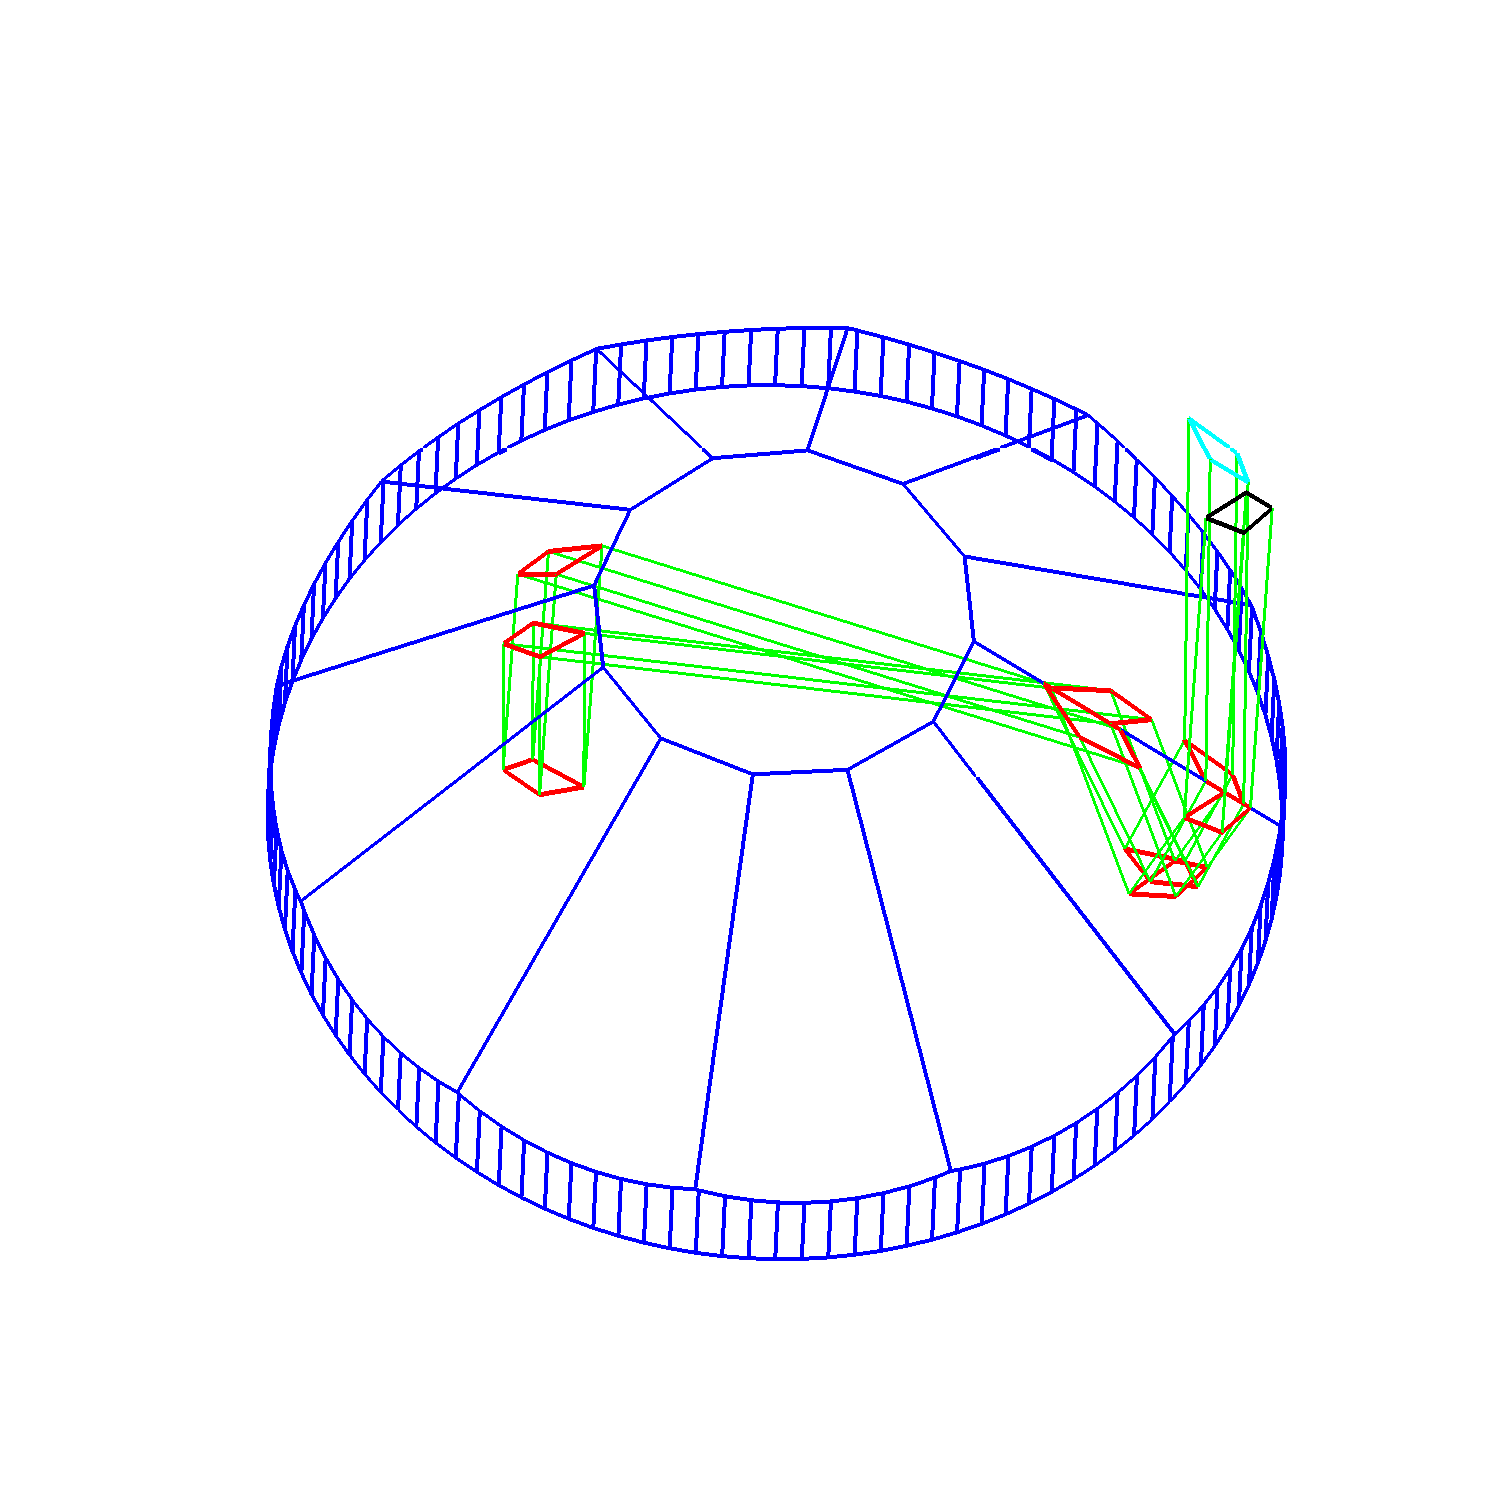
\includegraphics[width=\textwidth]{group9I.pdf}
\end{minipage}
\caption{3D view of ray example in classes 9J.}
\label{fig:modelClass3D1}
\end{figure}


\begin{figure}[htps]
\centering
\begin{minipage}[c]{0.325\textwidth}
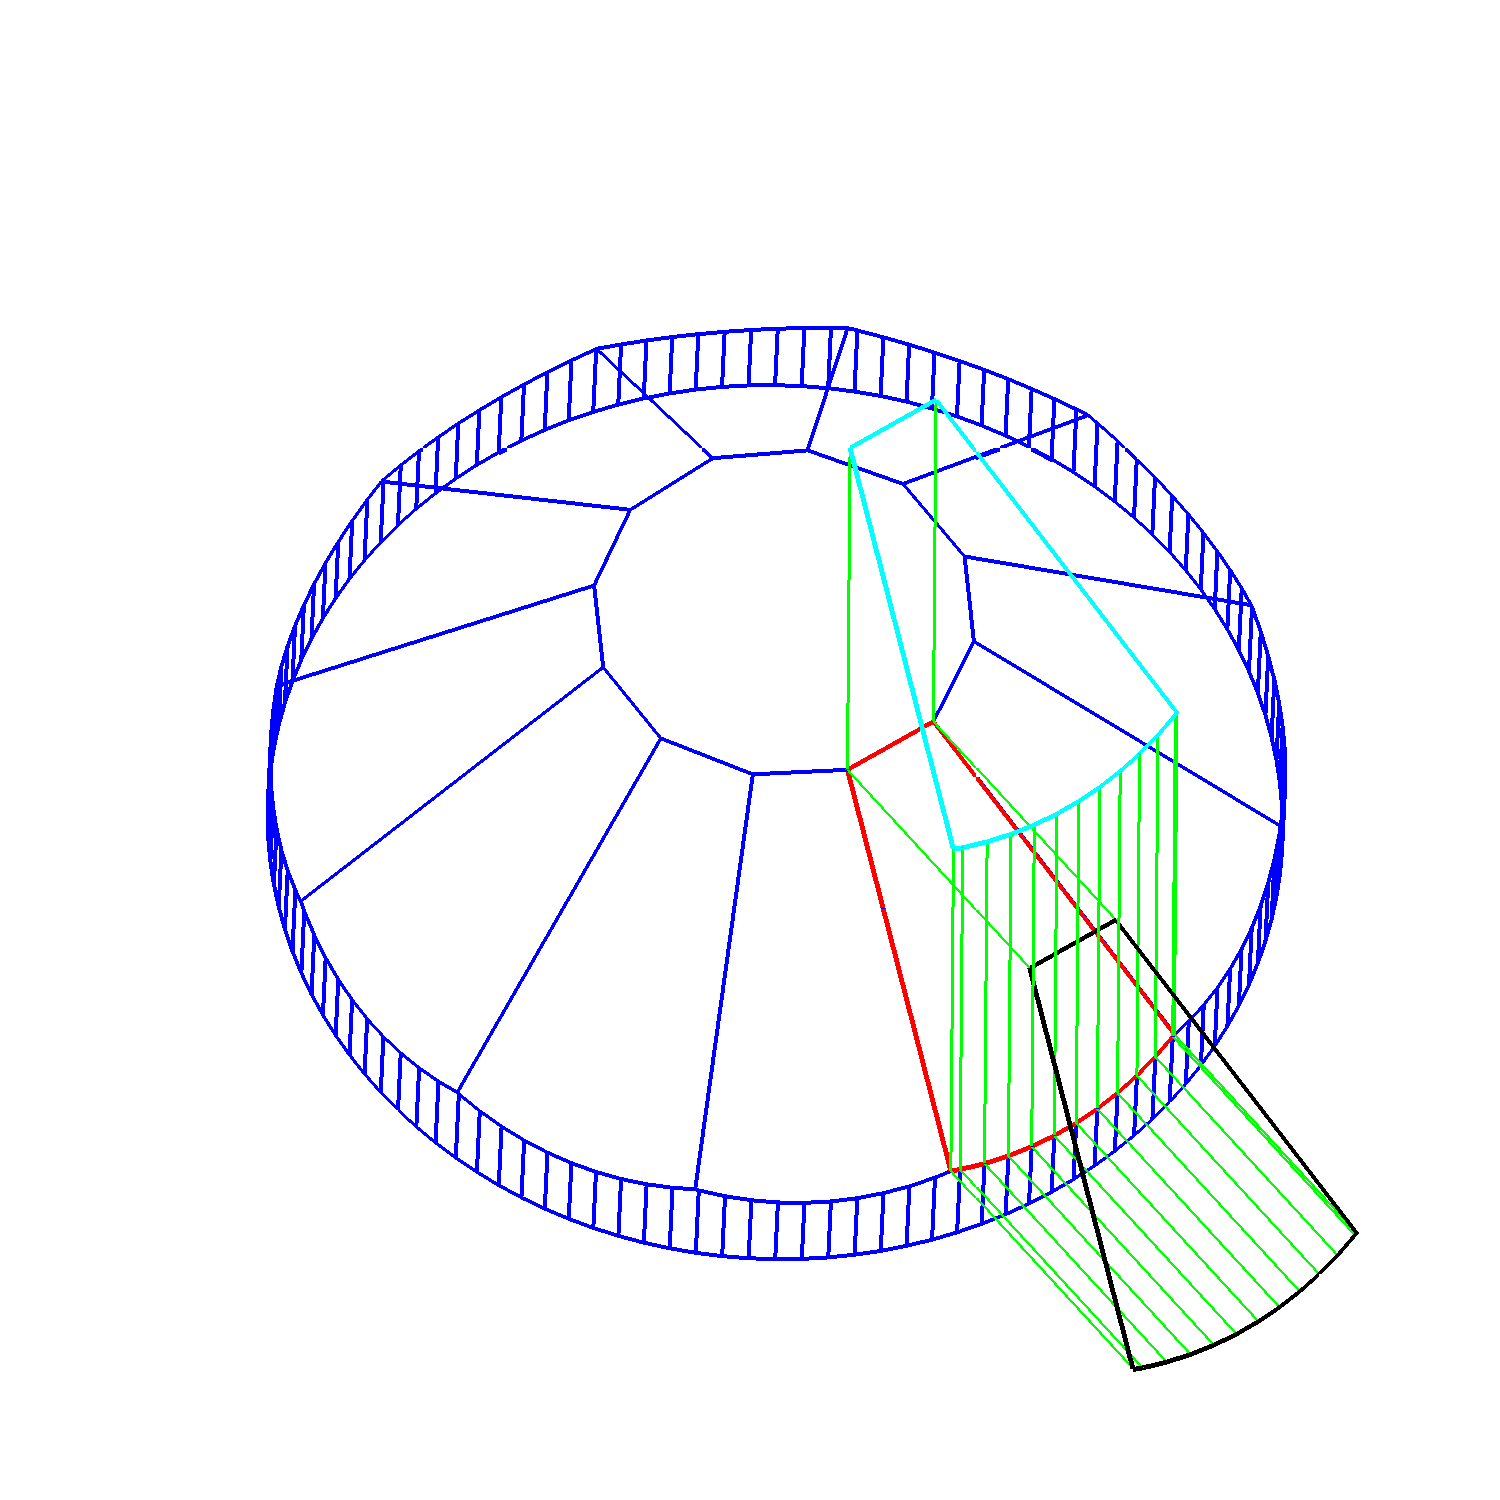
\includegraphics[width=\textwidth]{group1A.pdf}
\end{minipage}
\begin{minipage}[c]{0.325\textwidth}
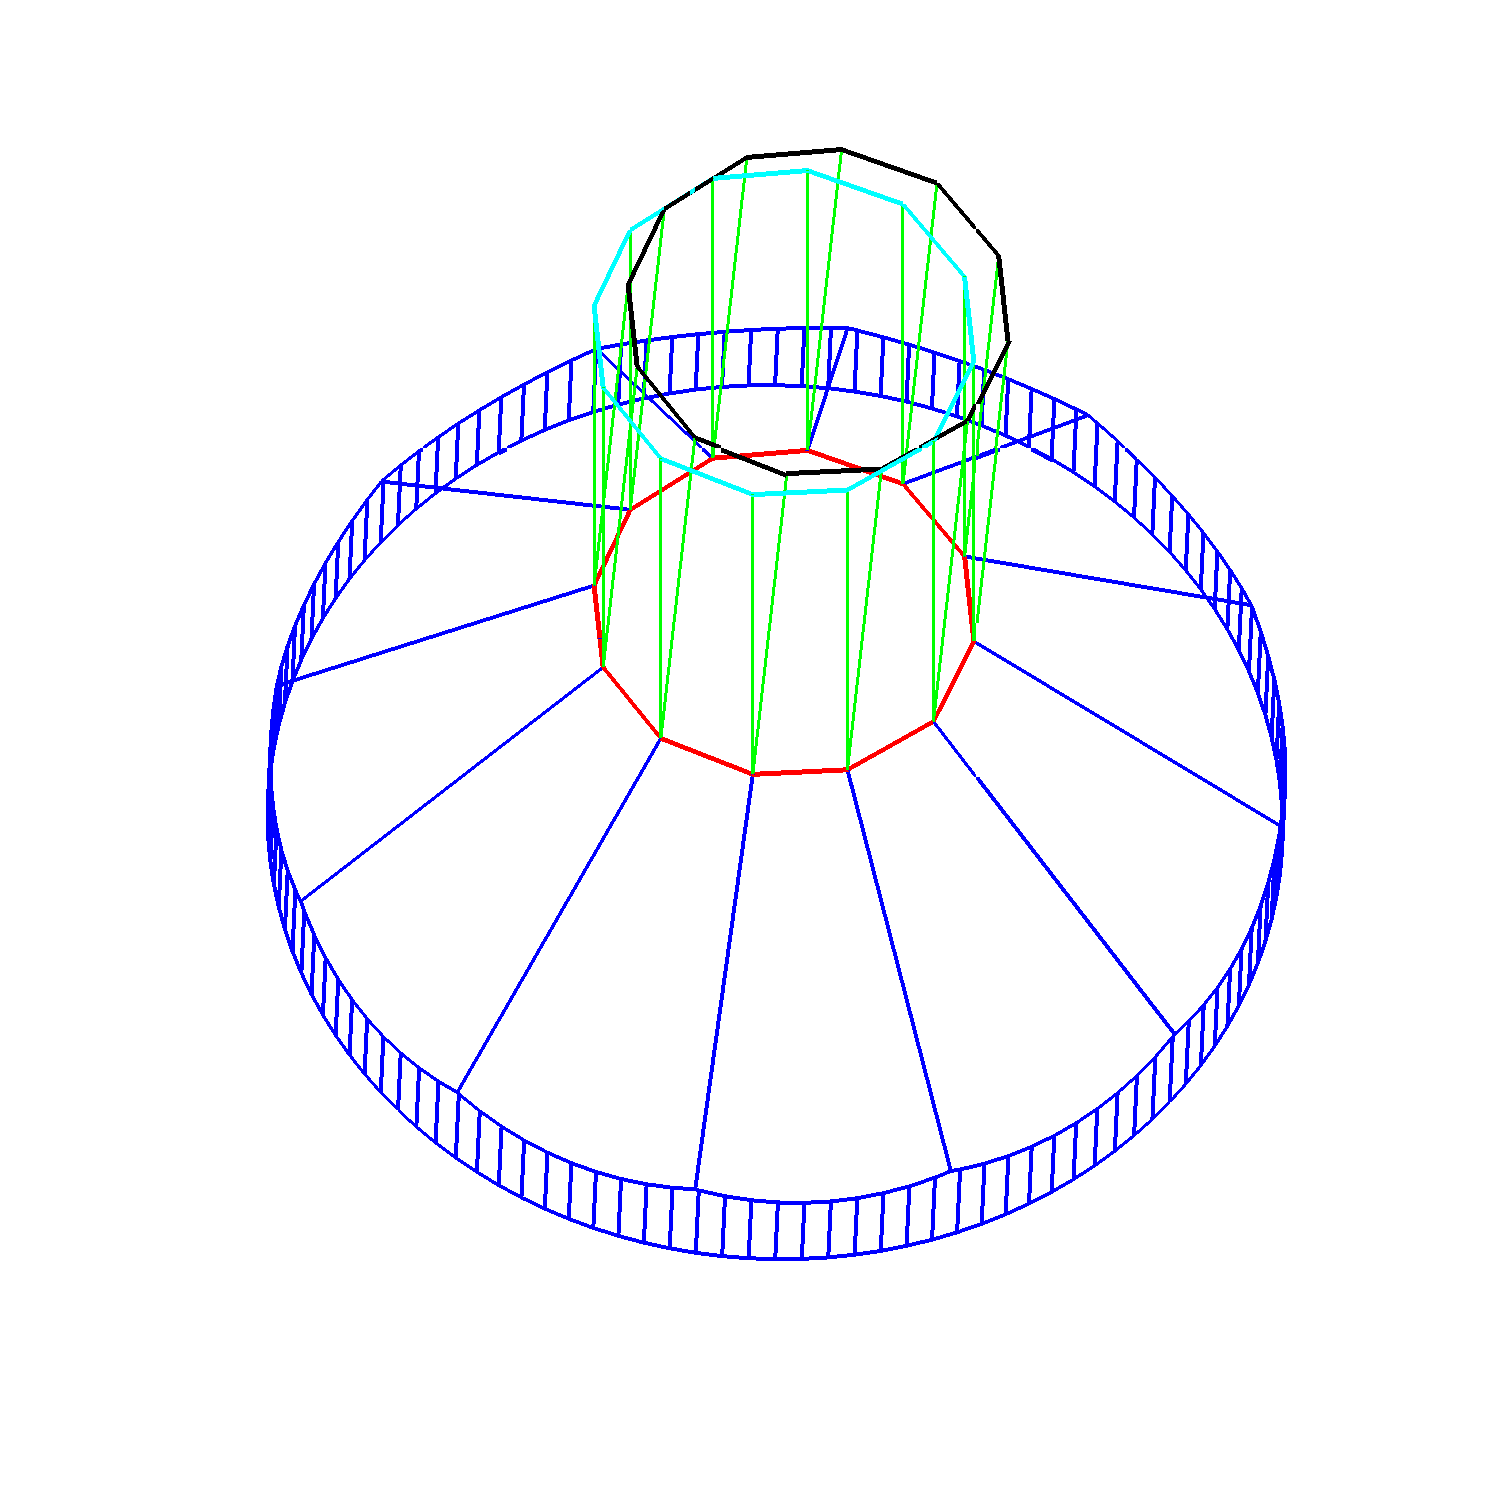
\includegraphics[width=\textwidth]{group1B.pdf}
\end{minipage}
\begin{minipage}[c]{0.325\textwidth}
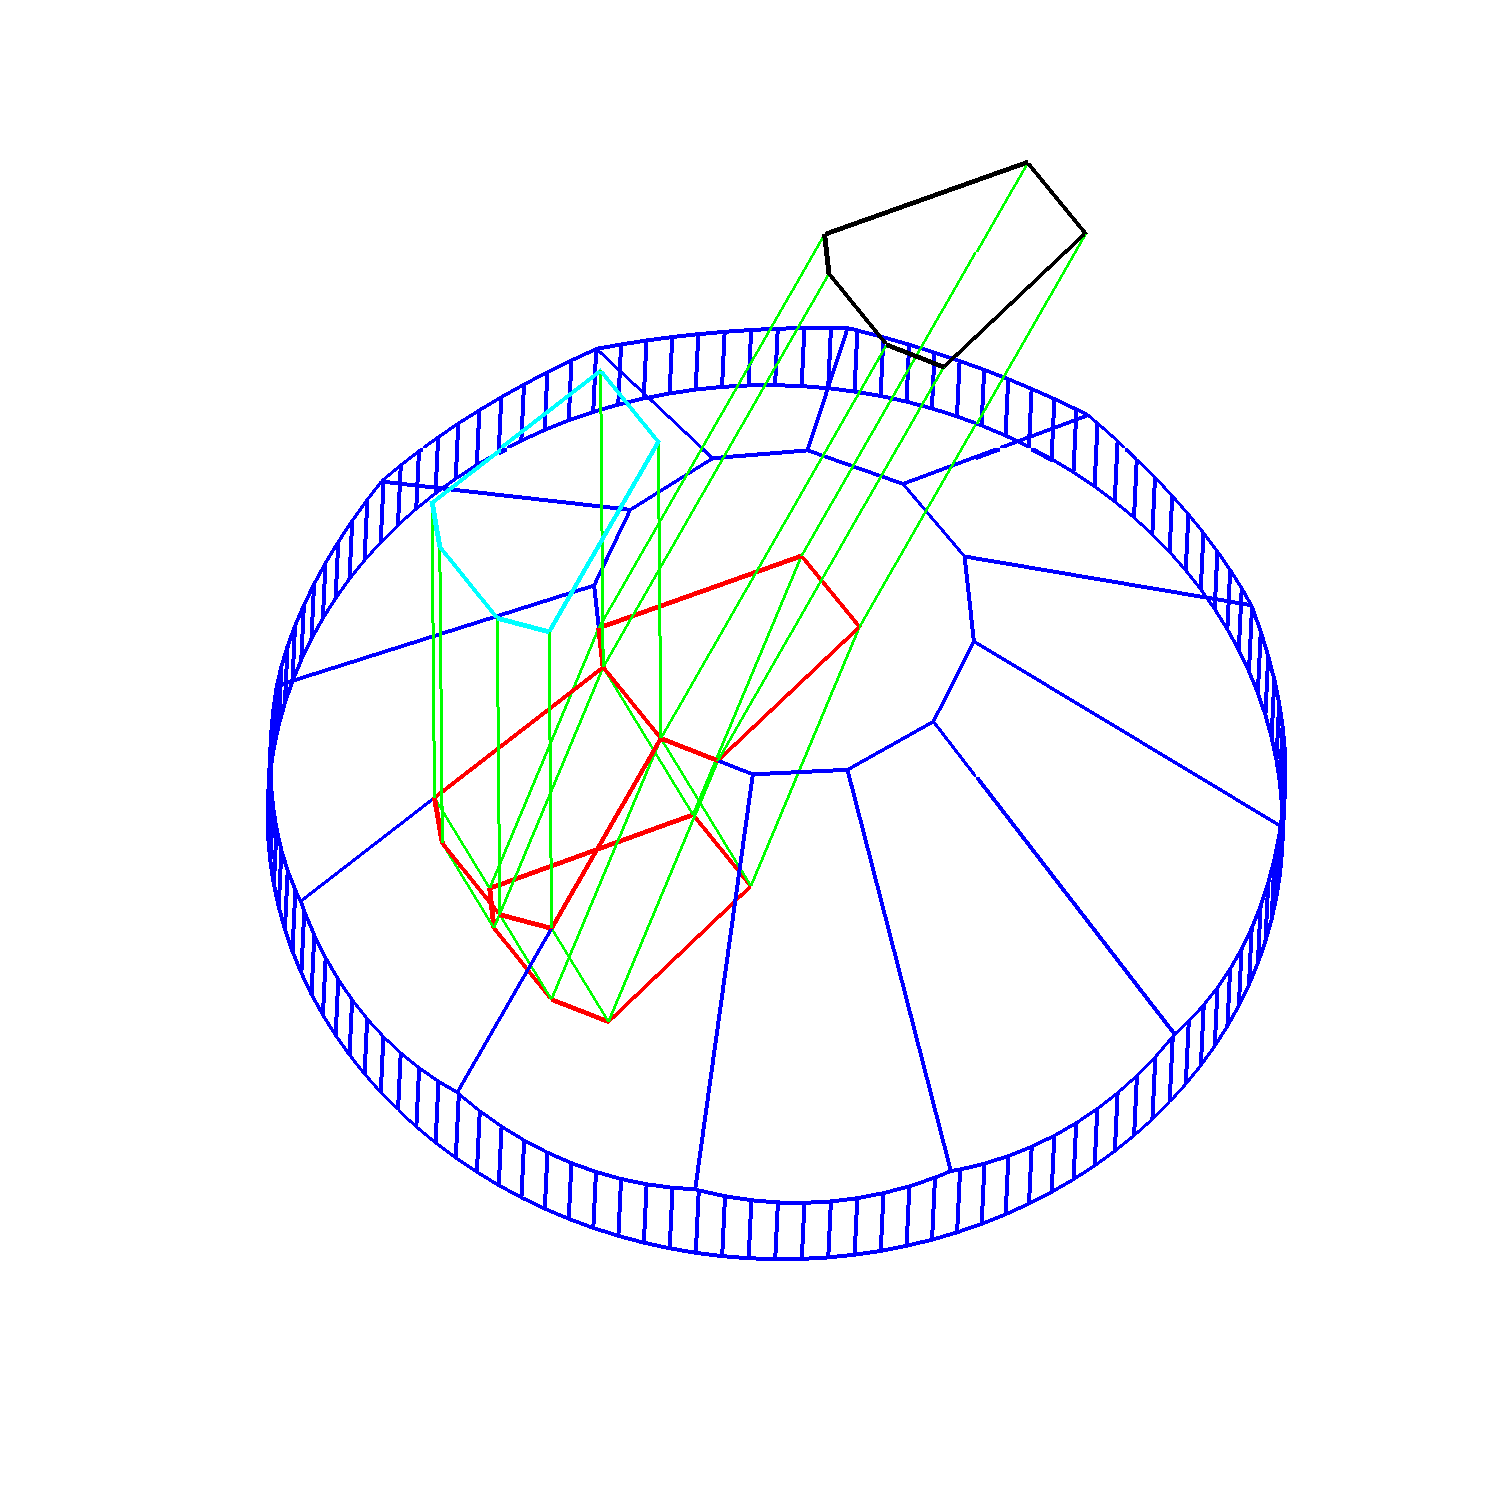
\includegraphics[width=\textwidth]{group3A.pdf}
\end{minipage}\\

\begin{minipage}[c]{0.325\textwidth}
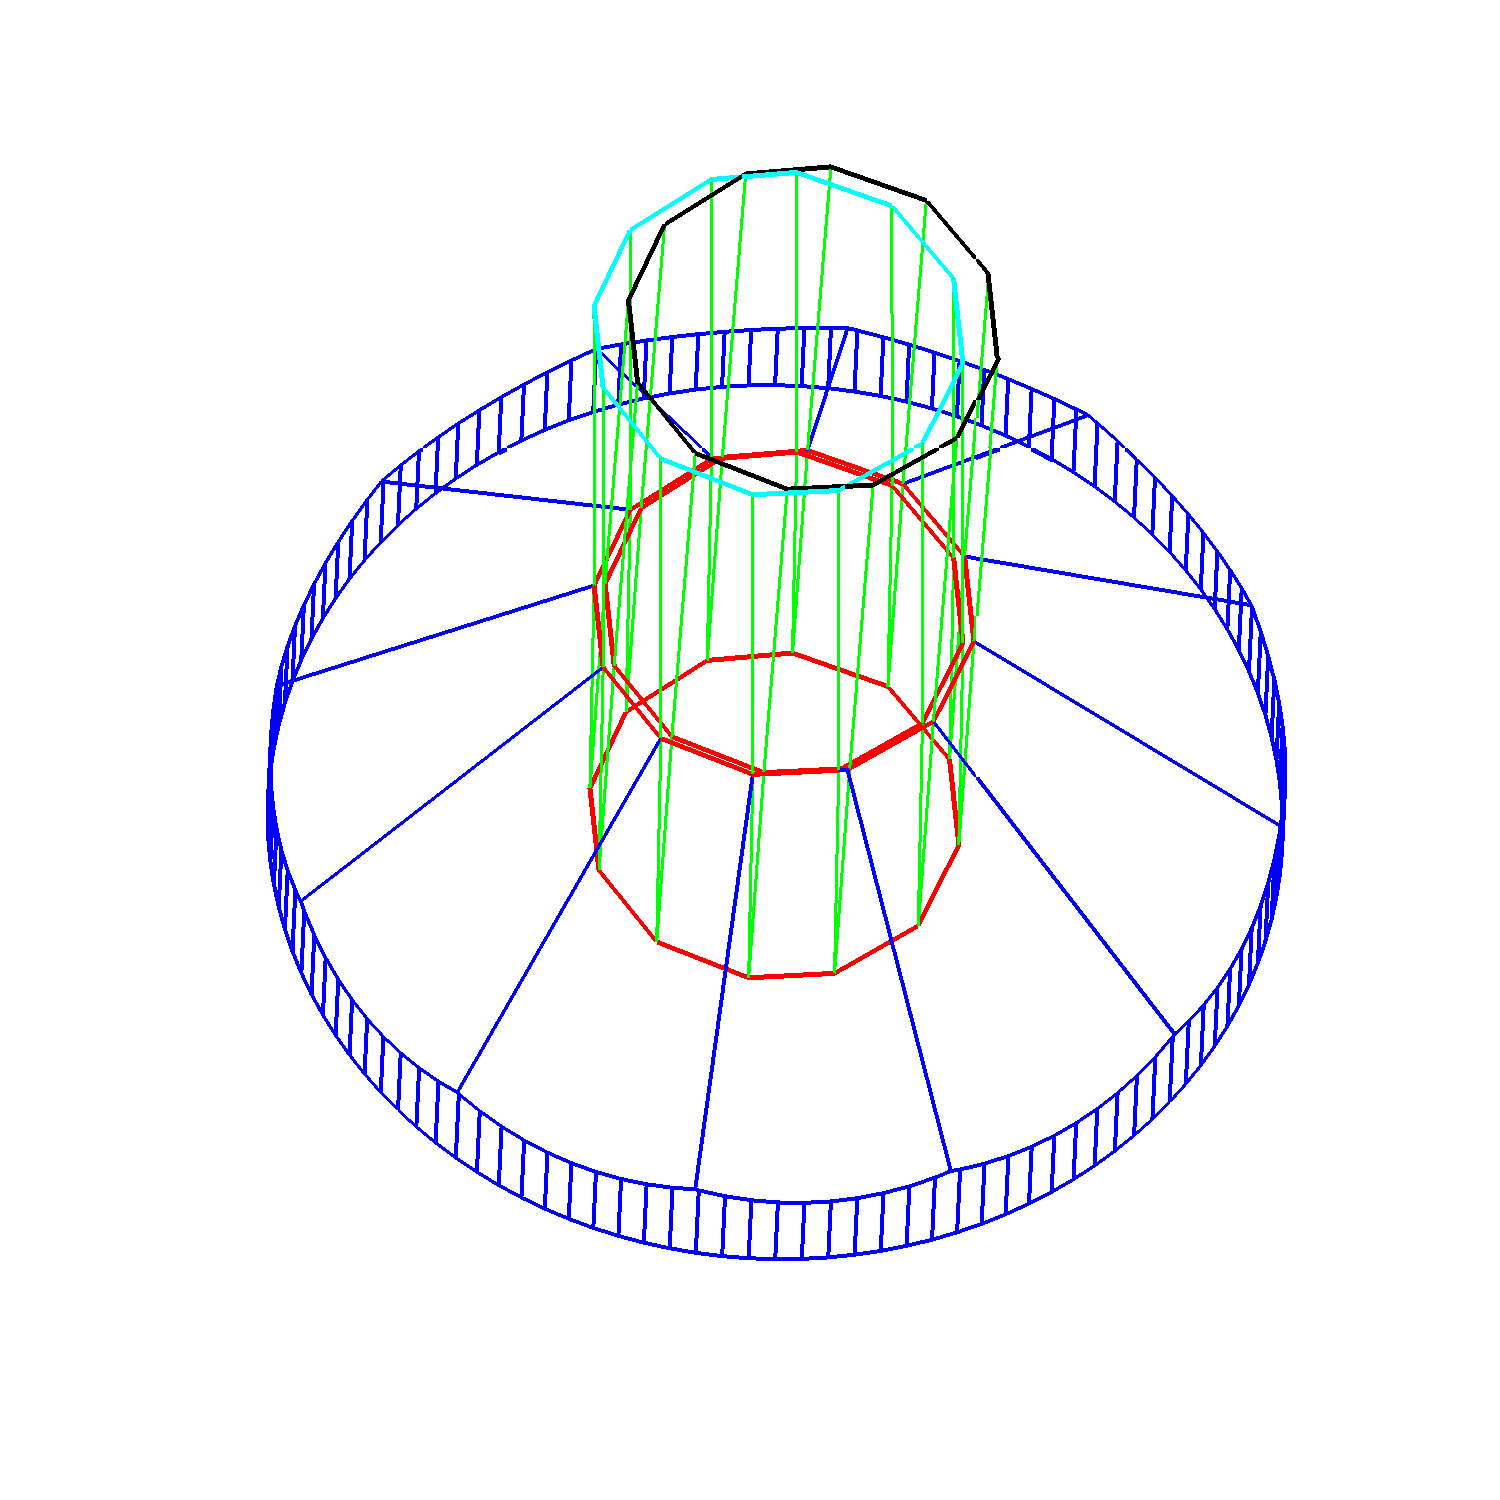
\includegraphics[width=\textwidth]{group3B.pdf}
\end{minipage}
\begin{minipage}[c]{0.325\textwidth}
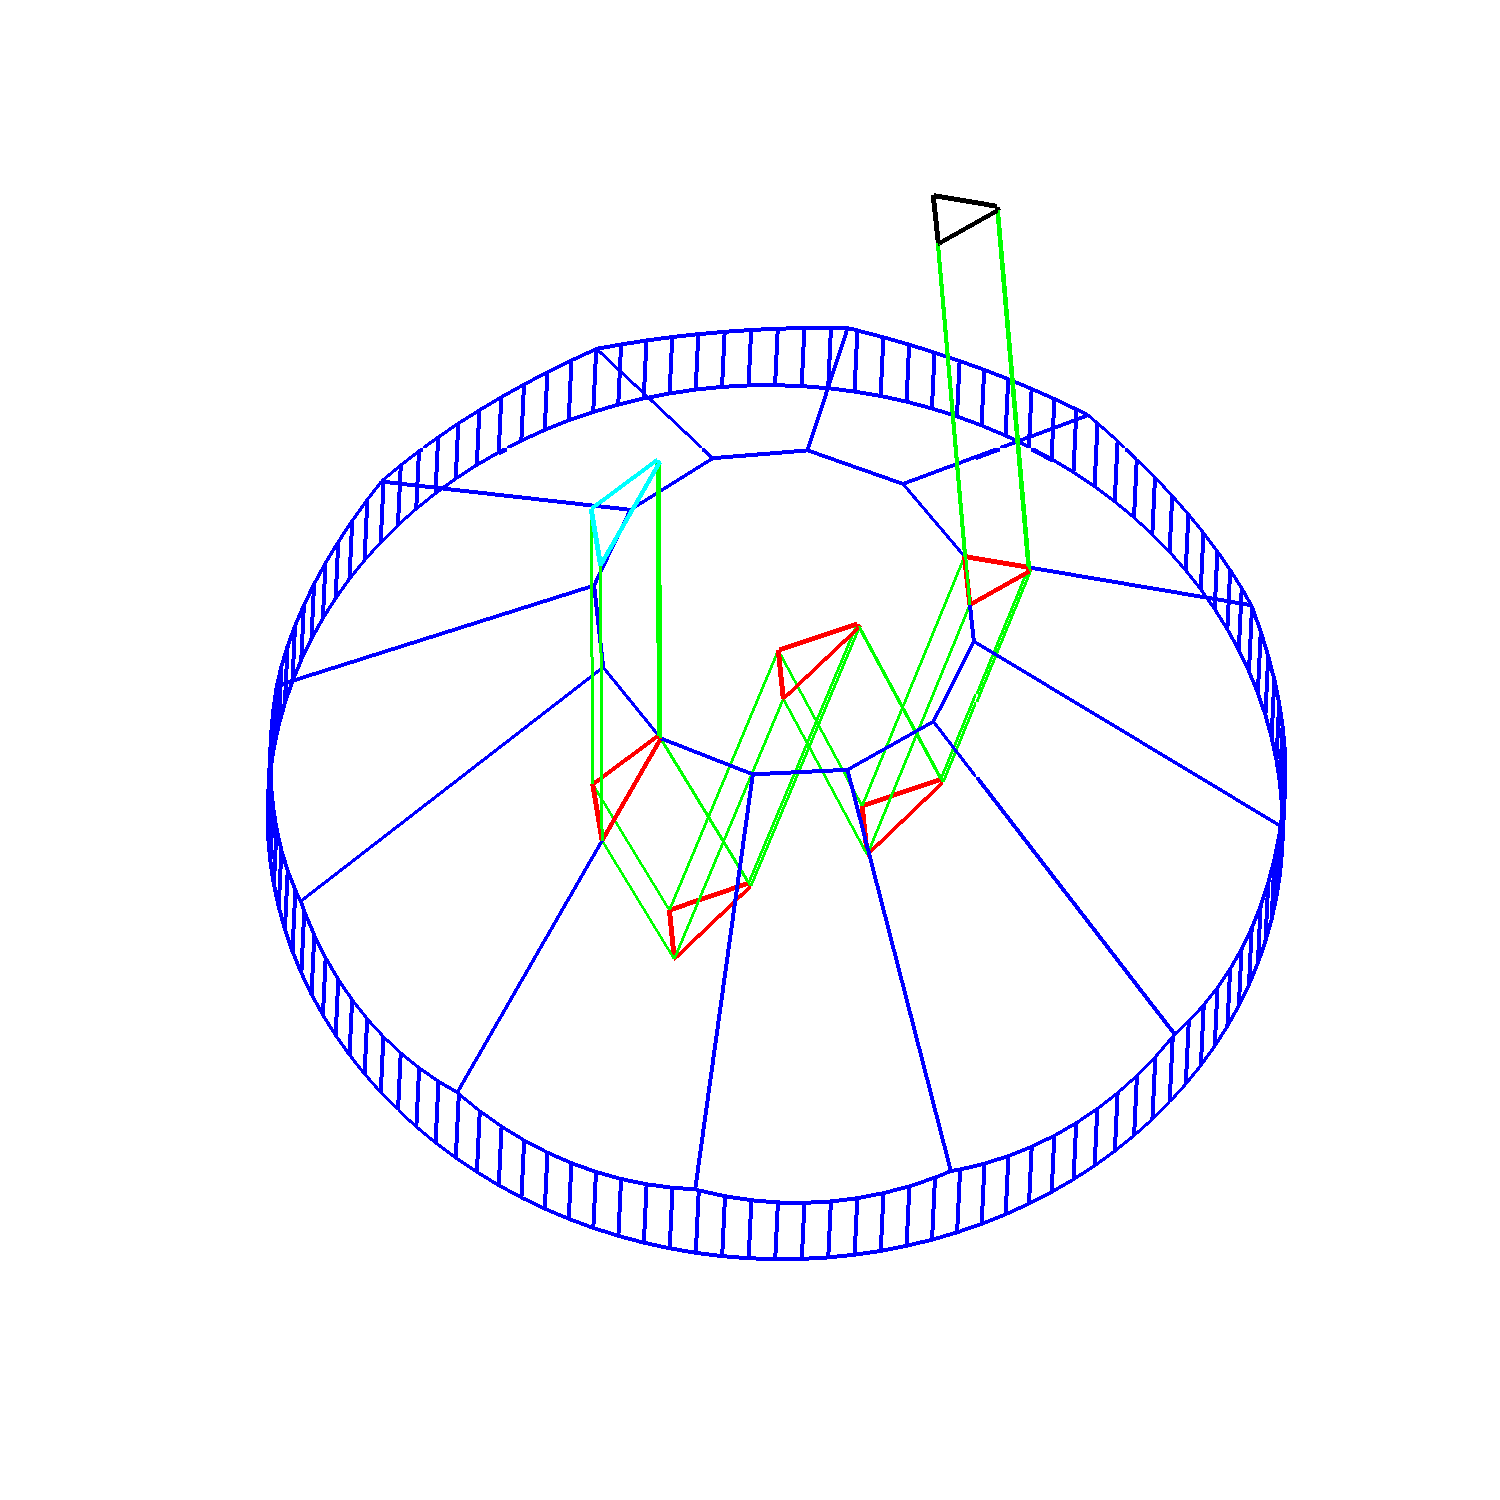
\includegraphics[width=\textwidth]{group5A.pdf}
\end{minipage}
\begin{minipage}[c]{0.325\textwidth}
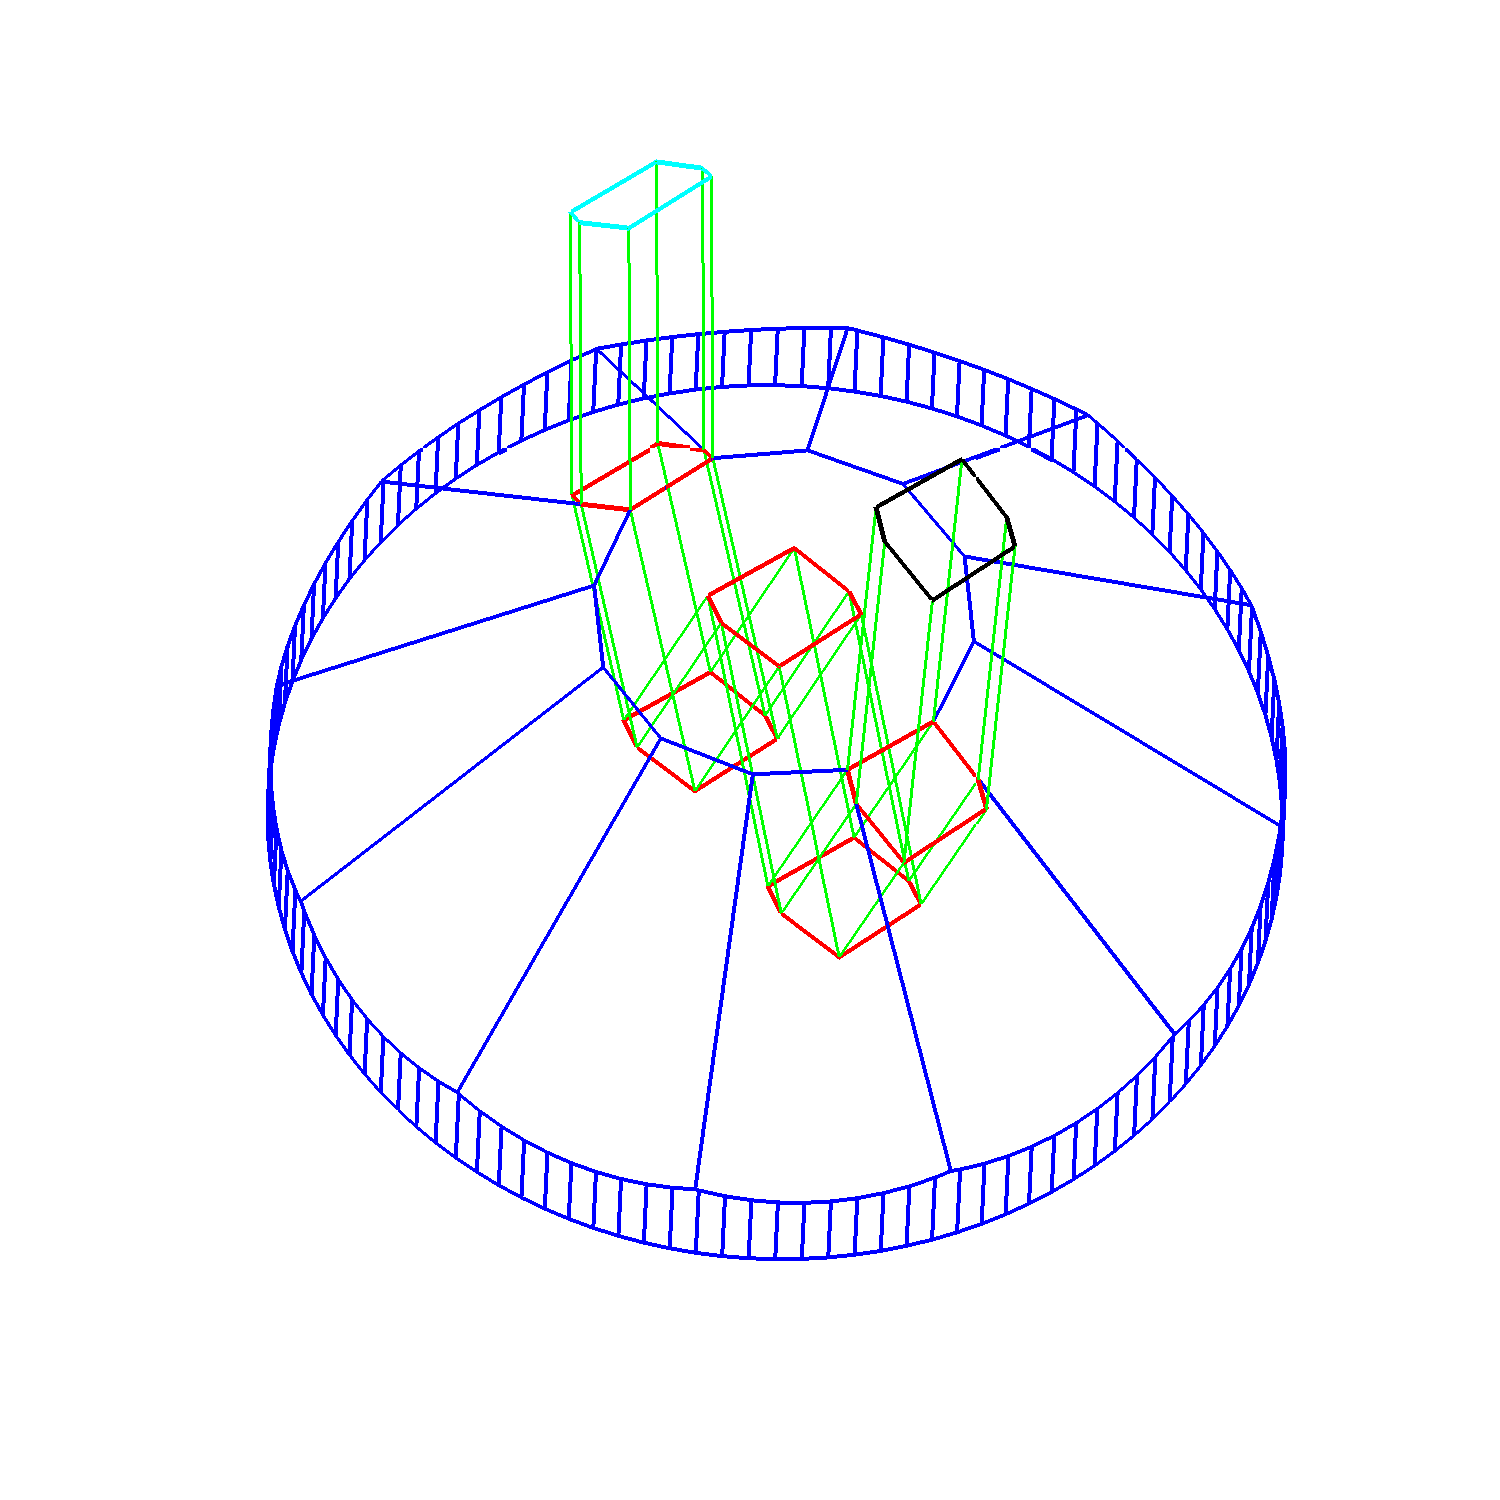
\includegraphics[width=\textwidth]{group5B.pdf}
\end{minipage}\\

\begin{minipage}[c]{0.325\textwidth}
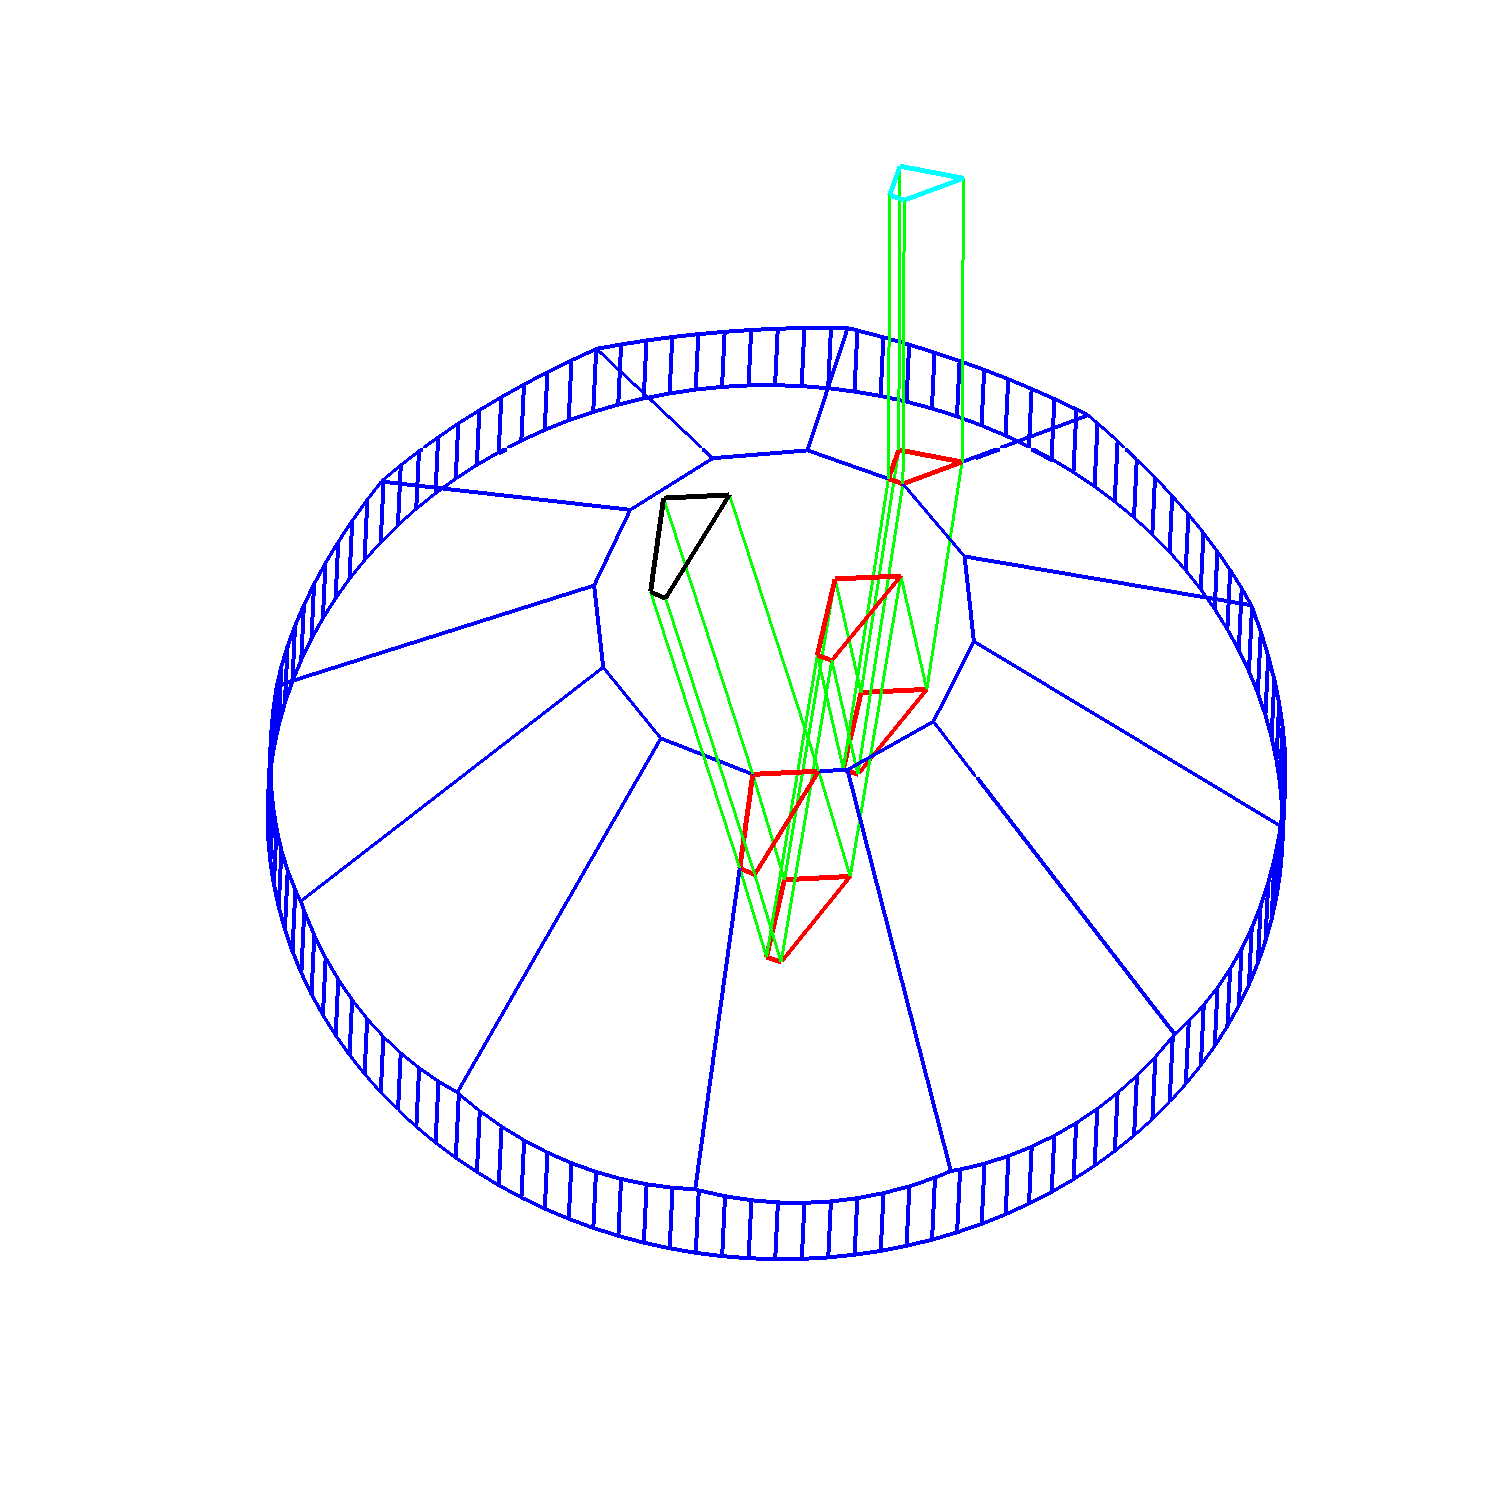
\includegraphics[width=\textwidth]{group5C.pdf}
\end{minipage}
\begin{minipage}[c]{0.325\textwidth}
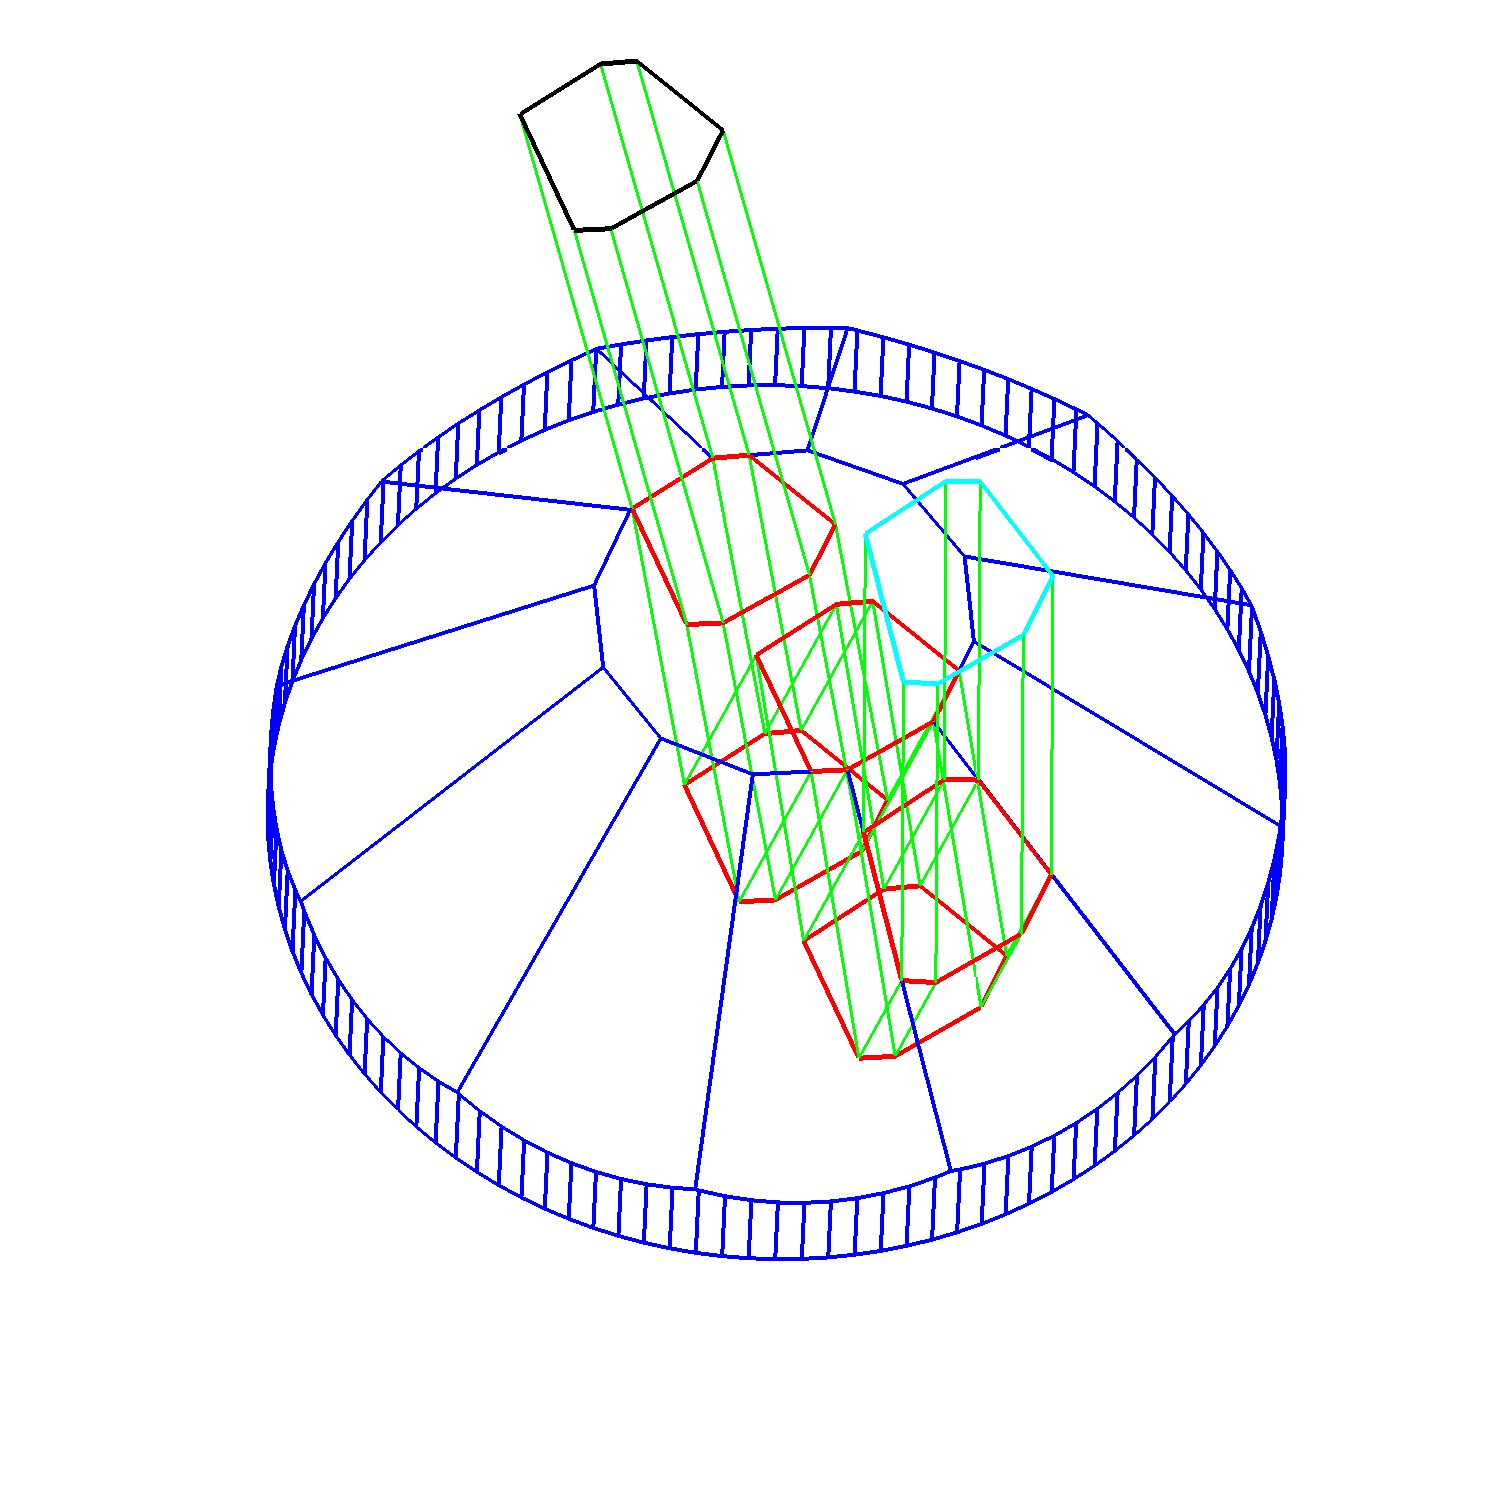
\includegraphics[width=\textwidth]{group5D.pdf}
\end{minipage}
\begin{minipage}[c]{0.325\textwidth}
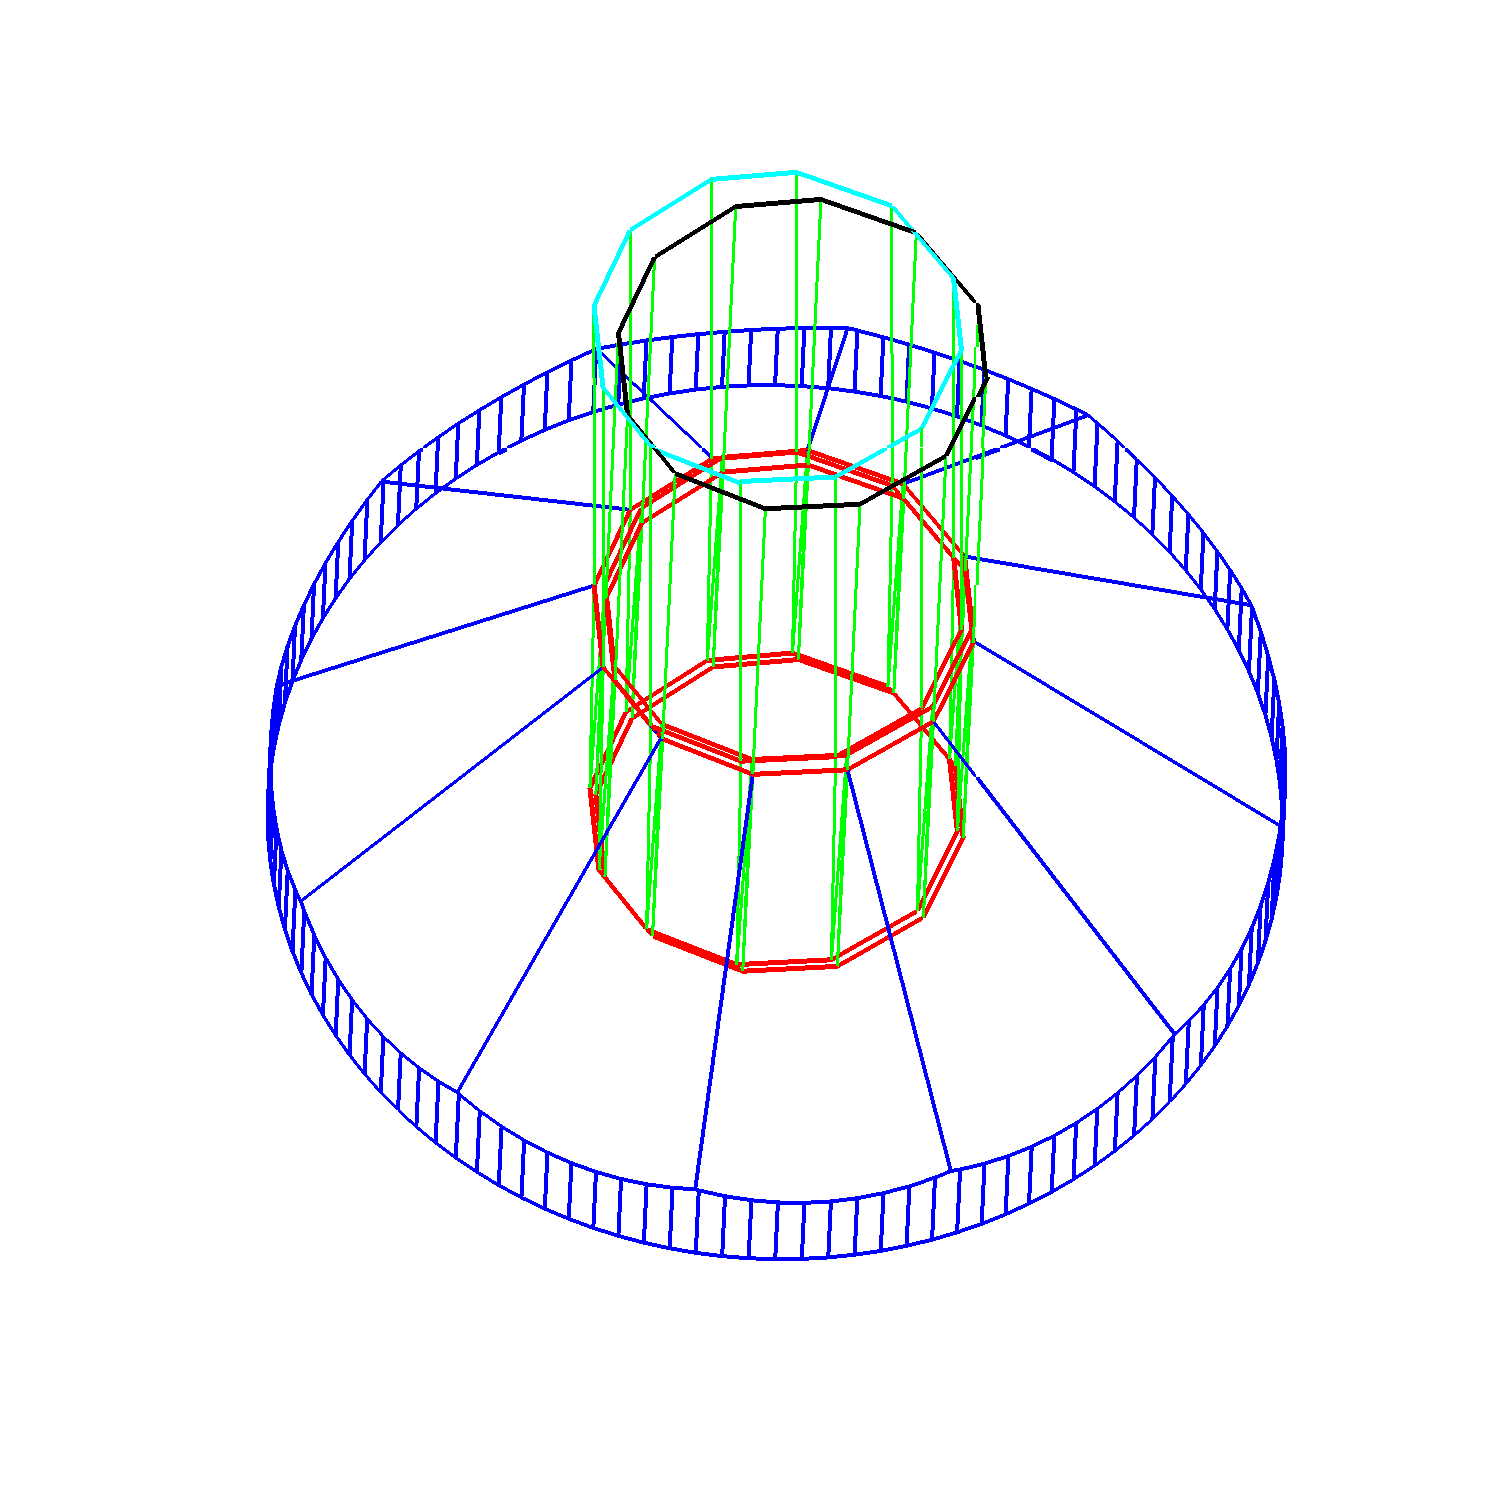
\includegraphics[width=\textwidth]{group5E.pdf}
\end{minipage}\\

\begin{minipage}[c]{0.325\textwidth}
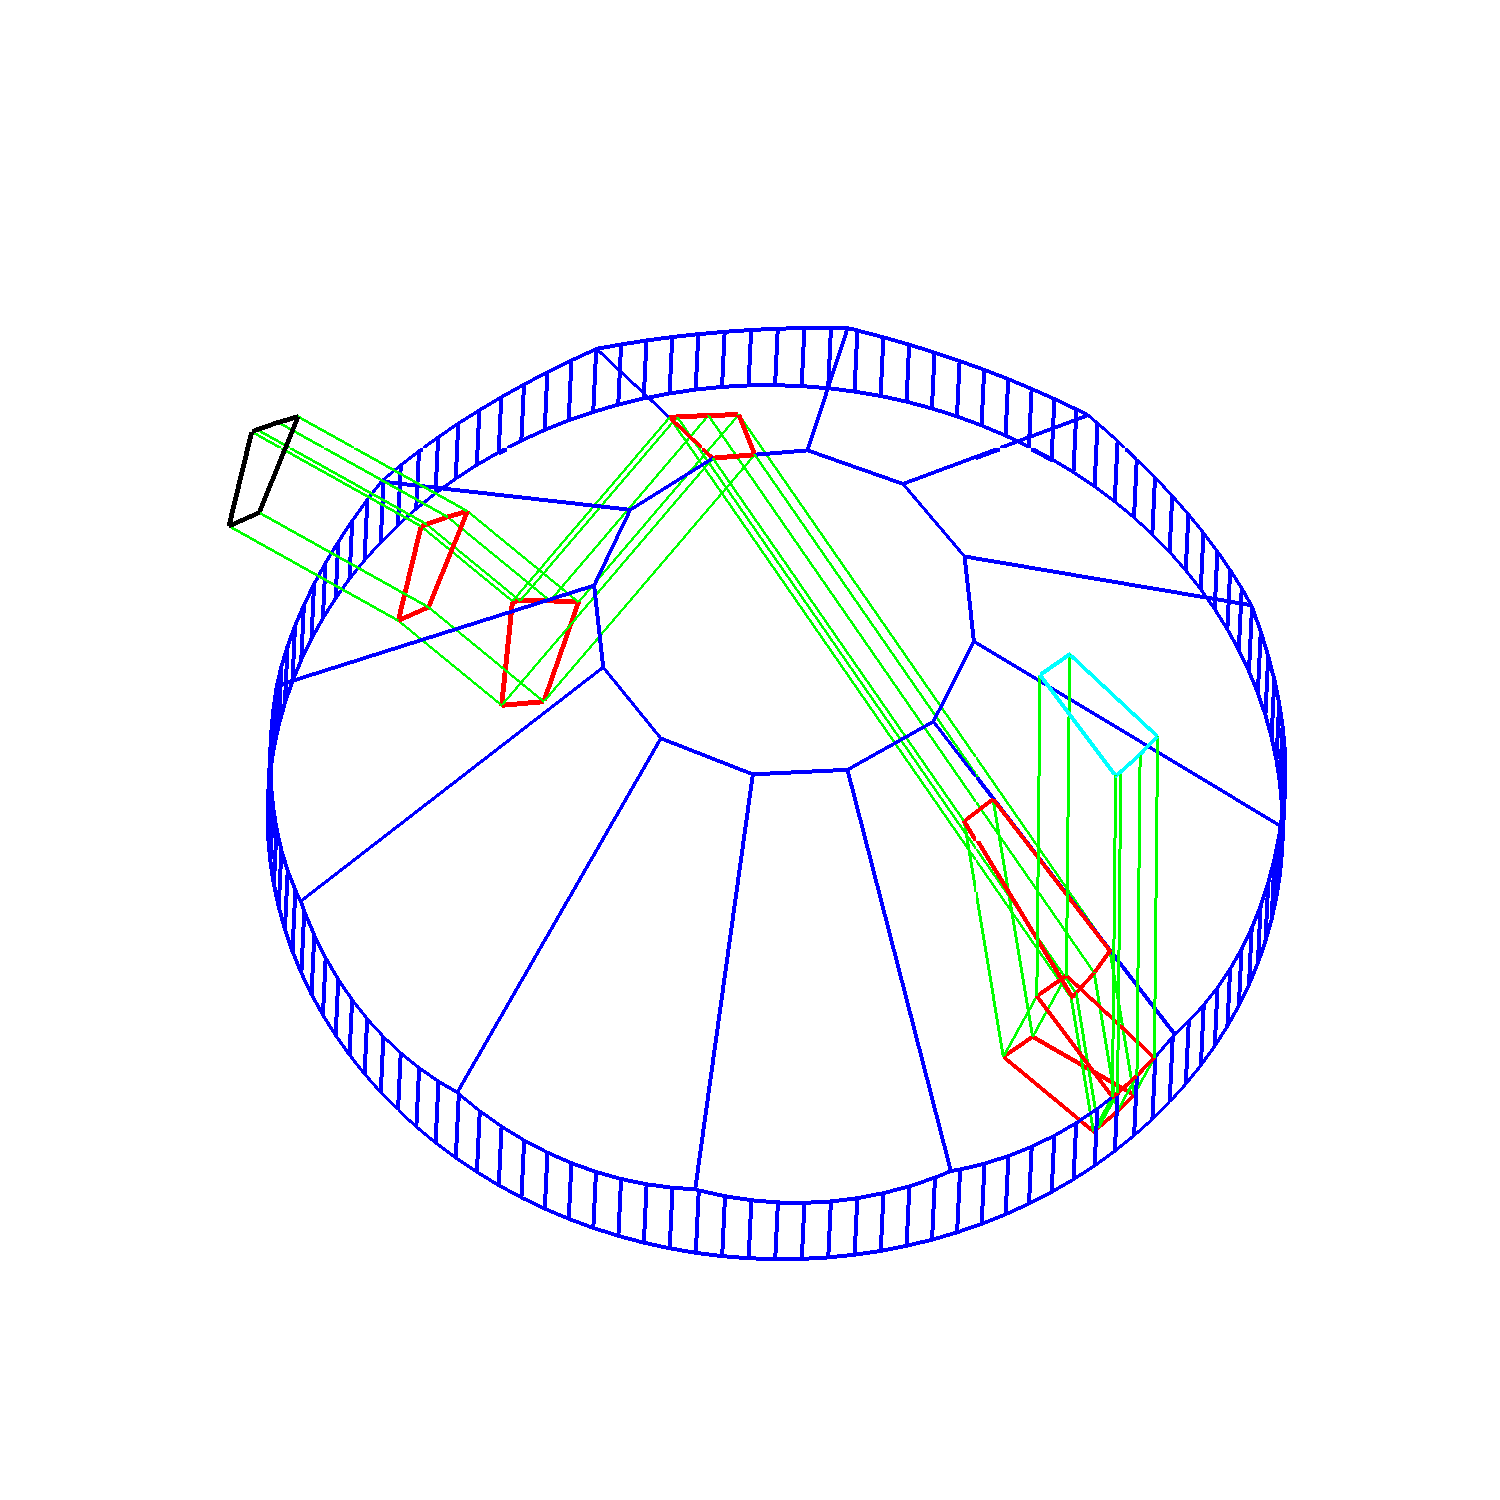
\includegraphics[width=\textwidth]{group6A.pdf}
\end{minipage}
\begin{minipage}[c]{0.325\textwidth}
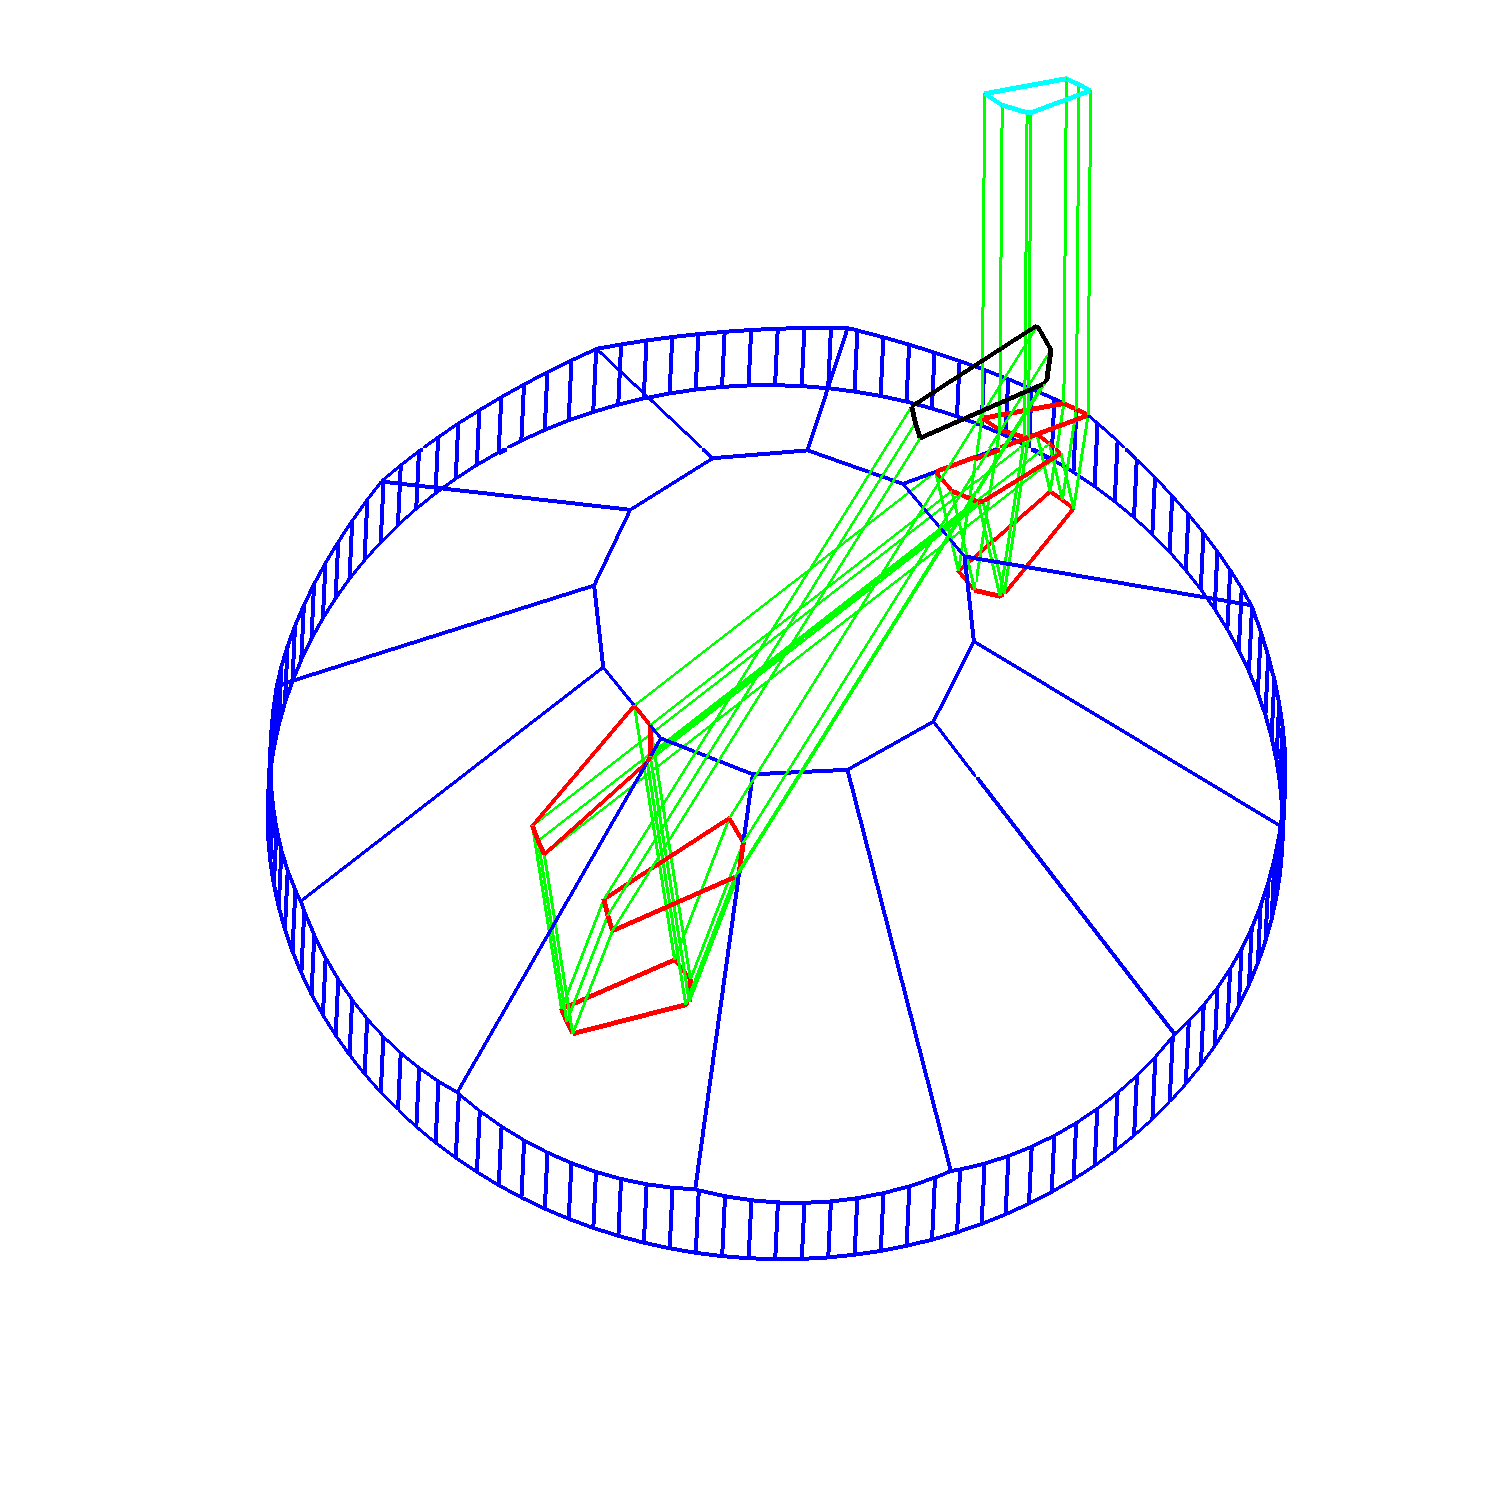
\includegraphics[width=\textwidth]{group6B.pdf}
\end{minipage}
\begin{minipage}[c]{0.325\textwidth}
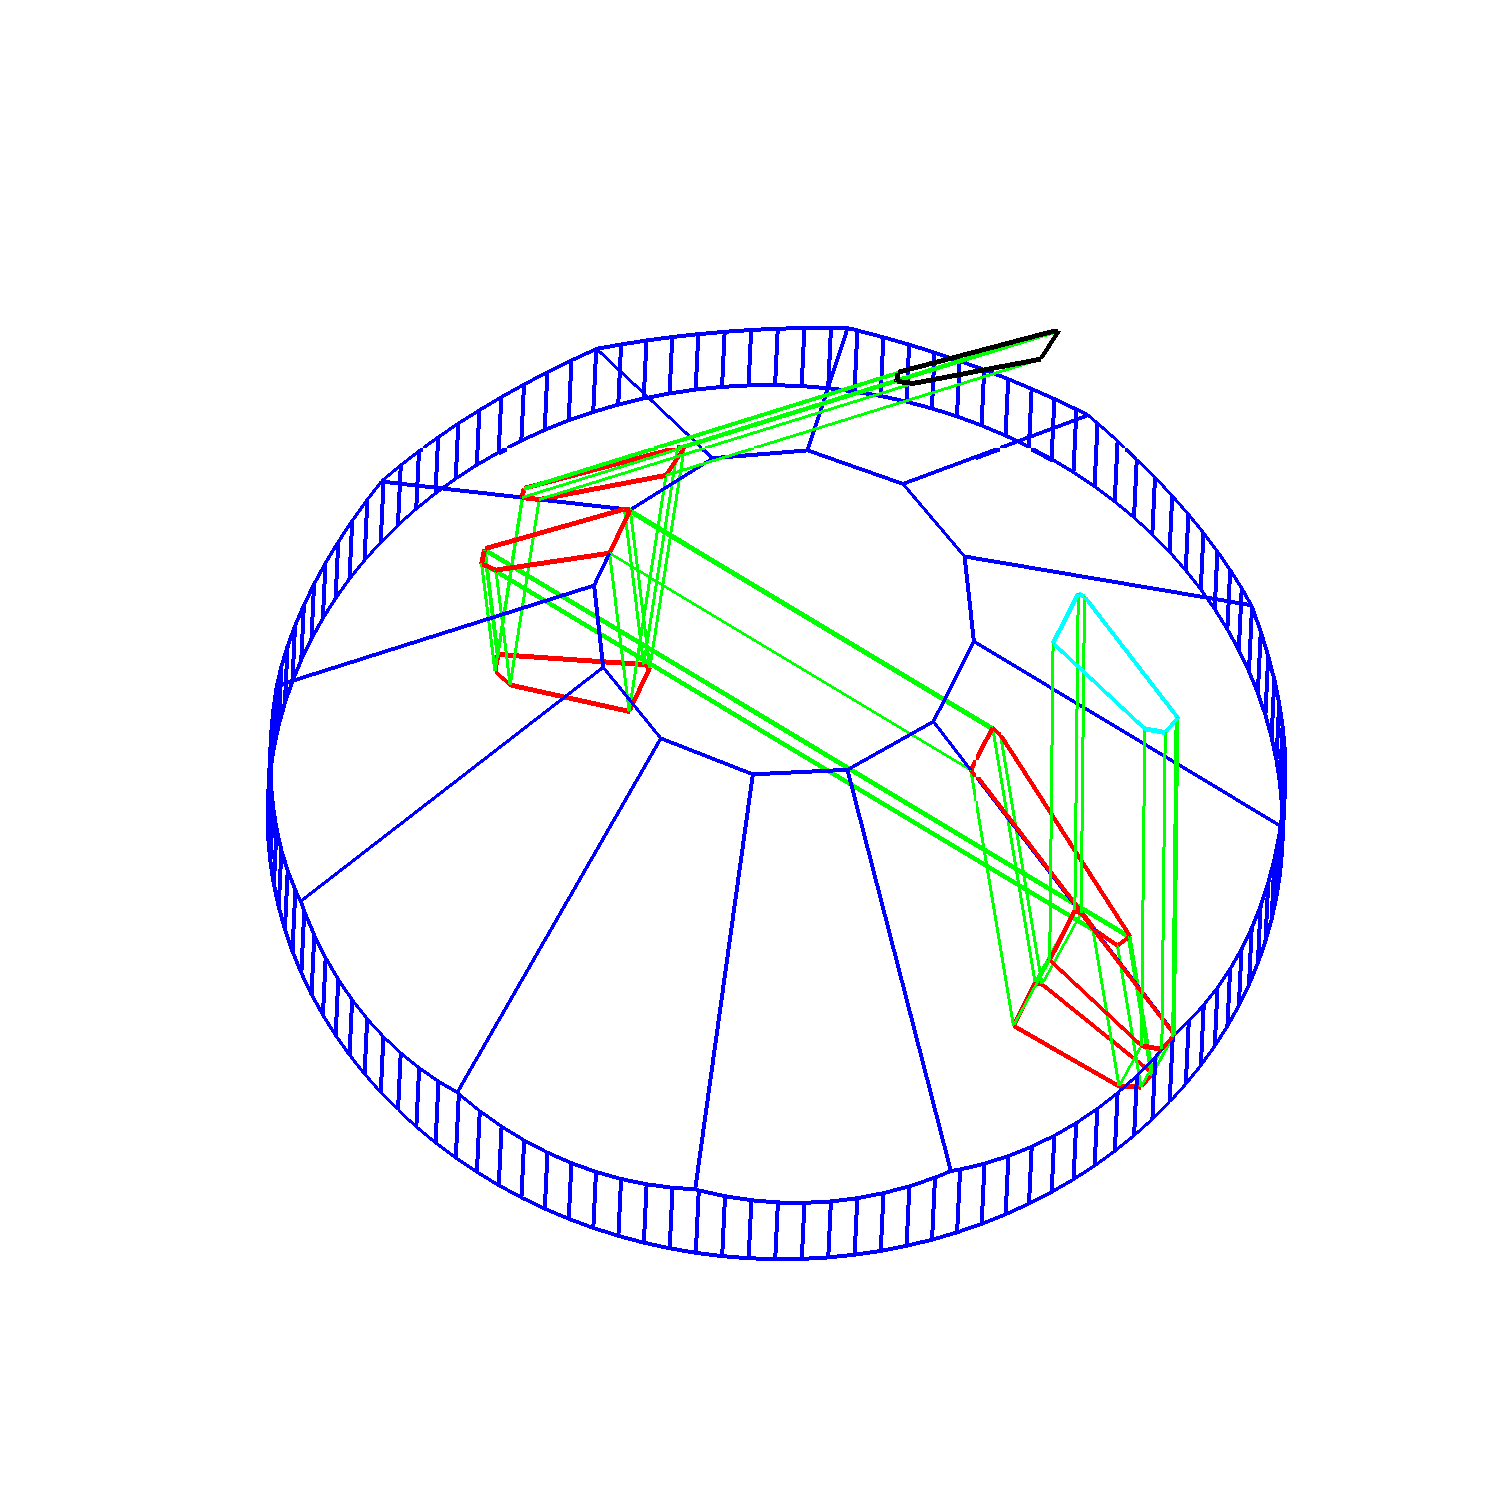
\includegraphics[width=\textwidth]{group6C.pdf}
\end{minipage}

\caption{3D view of ray example in classes 1A, 1B, 3A, 3B, 5A, 5B, 5C, 5D, 5E, 6A and 6B.}
\label{fig:modelClass3D1}
\end{figure}



\begin{figure}[htps]
\centering
\begin{minipage}[c]{0.325\textwidth}
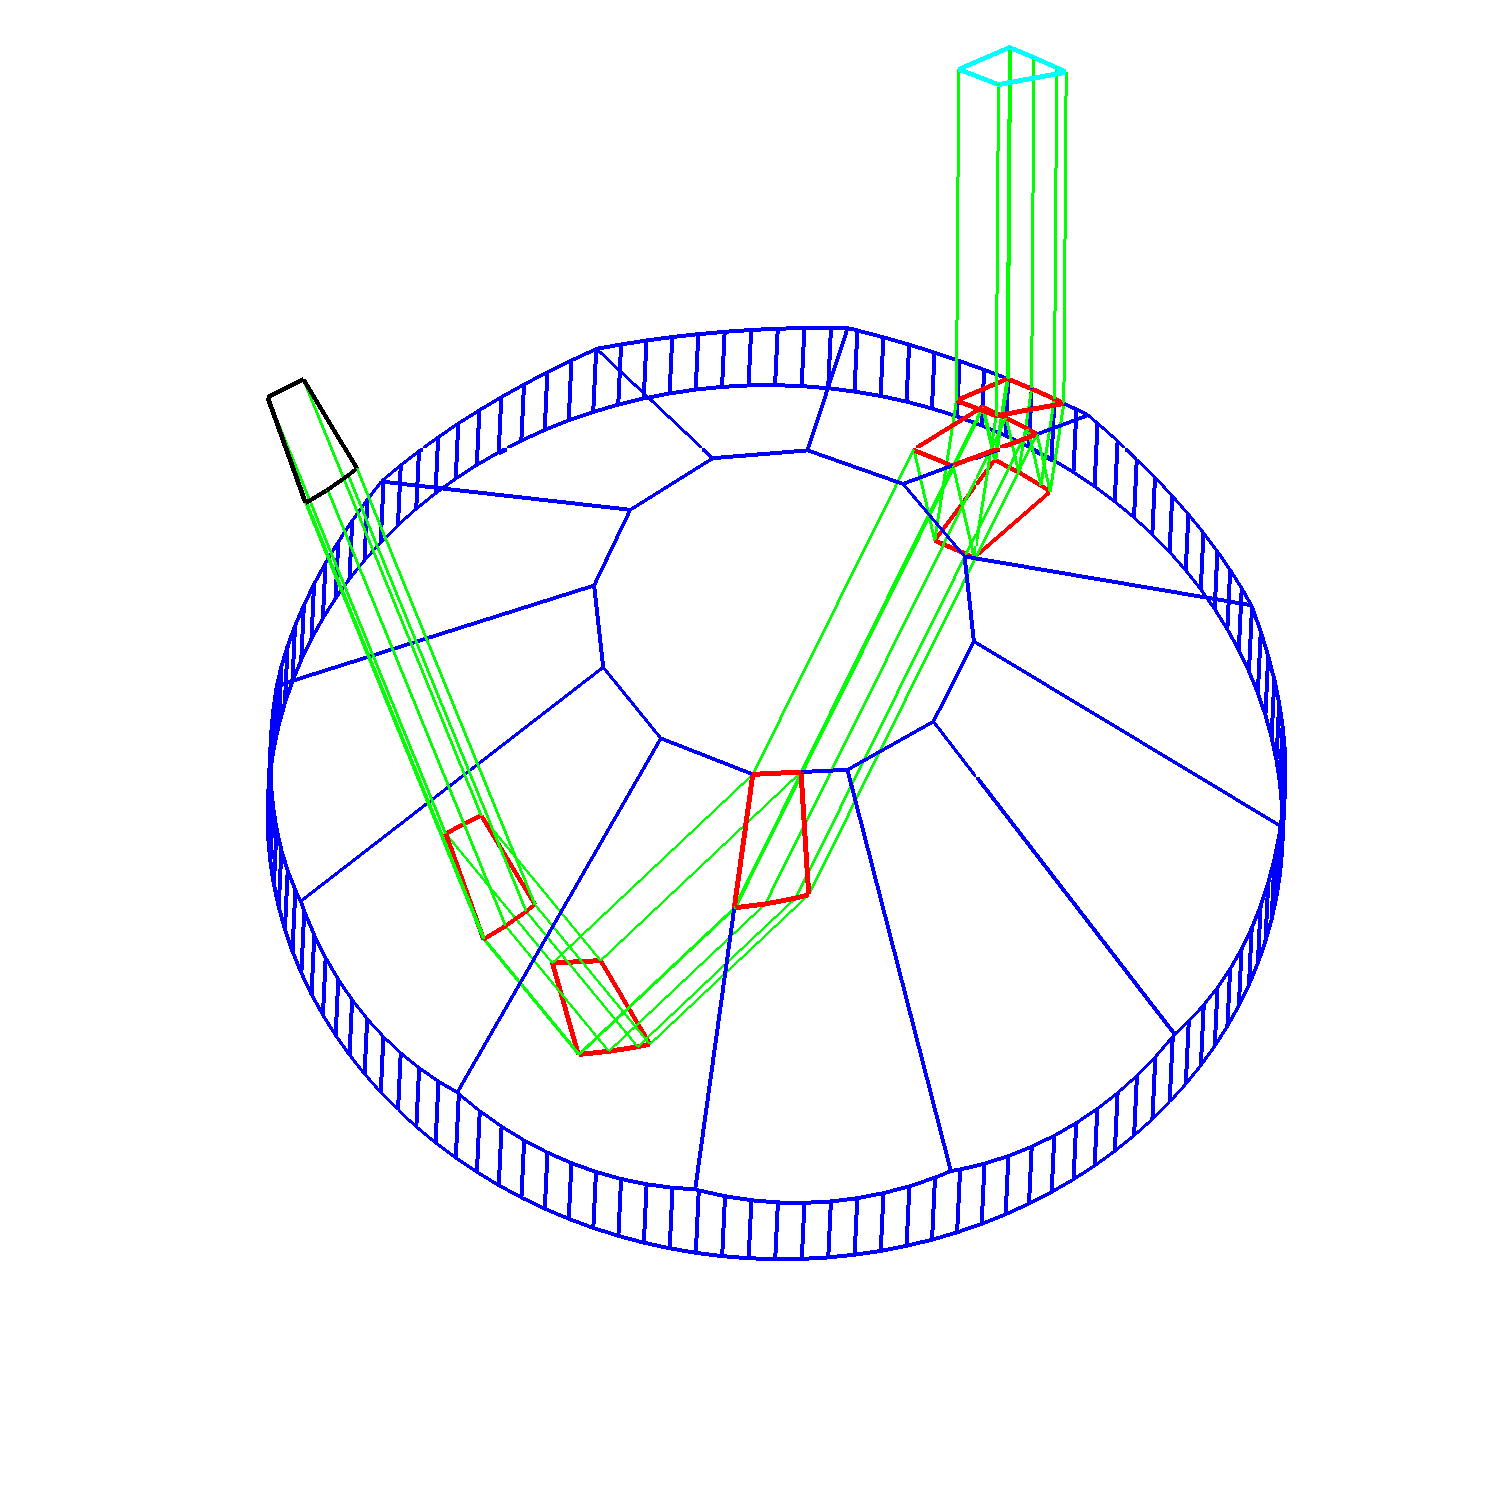
\includegraphics[width=\textwidth]{group6D.pdf}
\end{minipage}
\begin{minipage}[c]{0.325\textwidth}
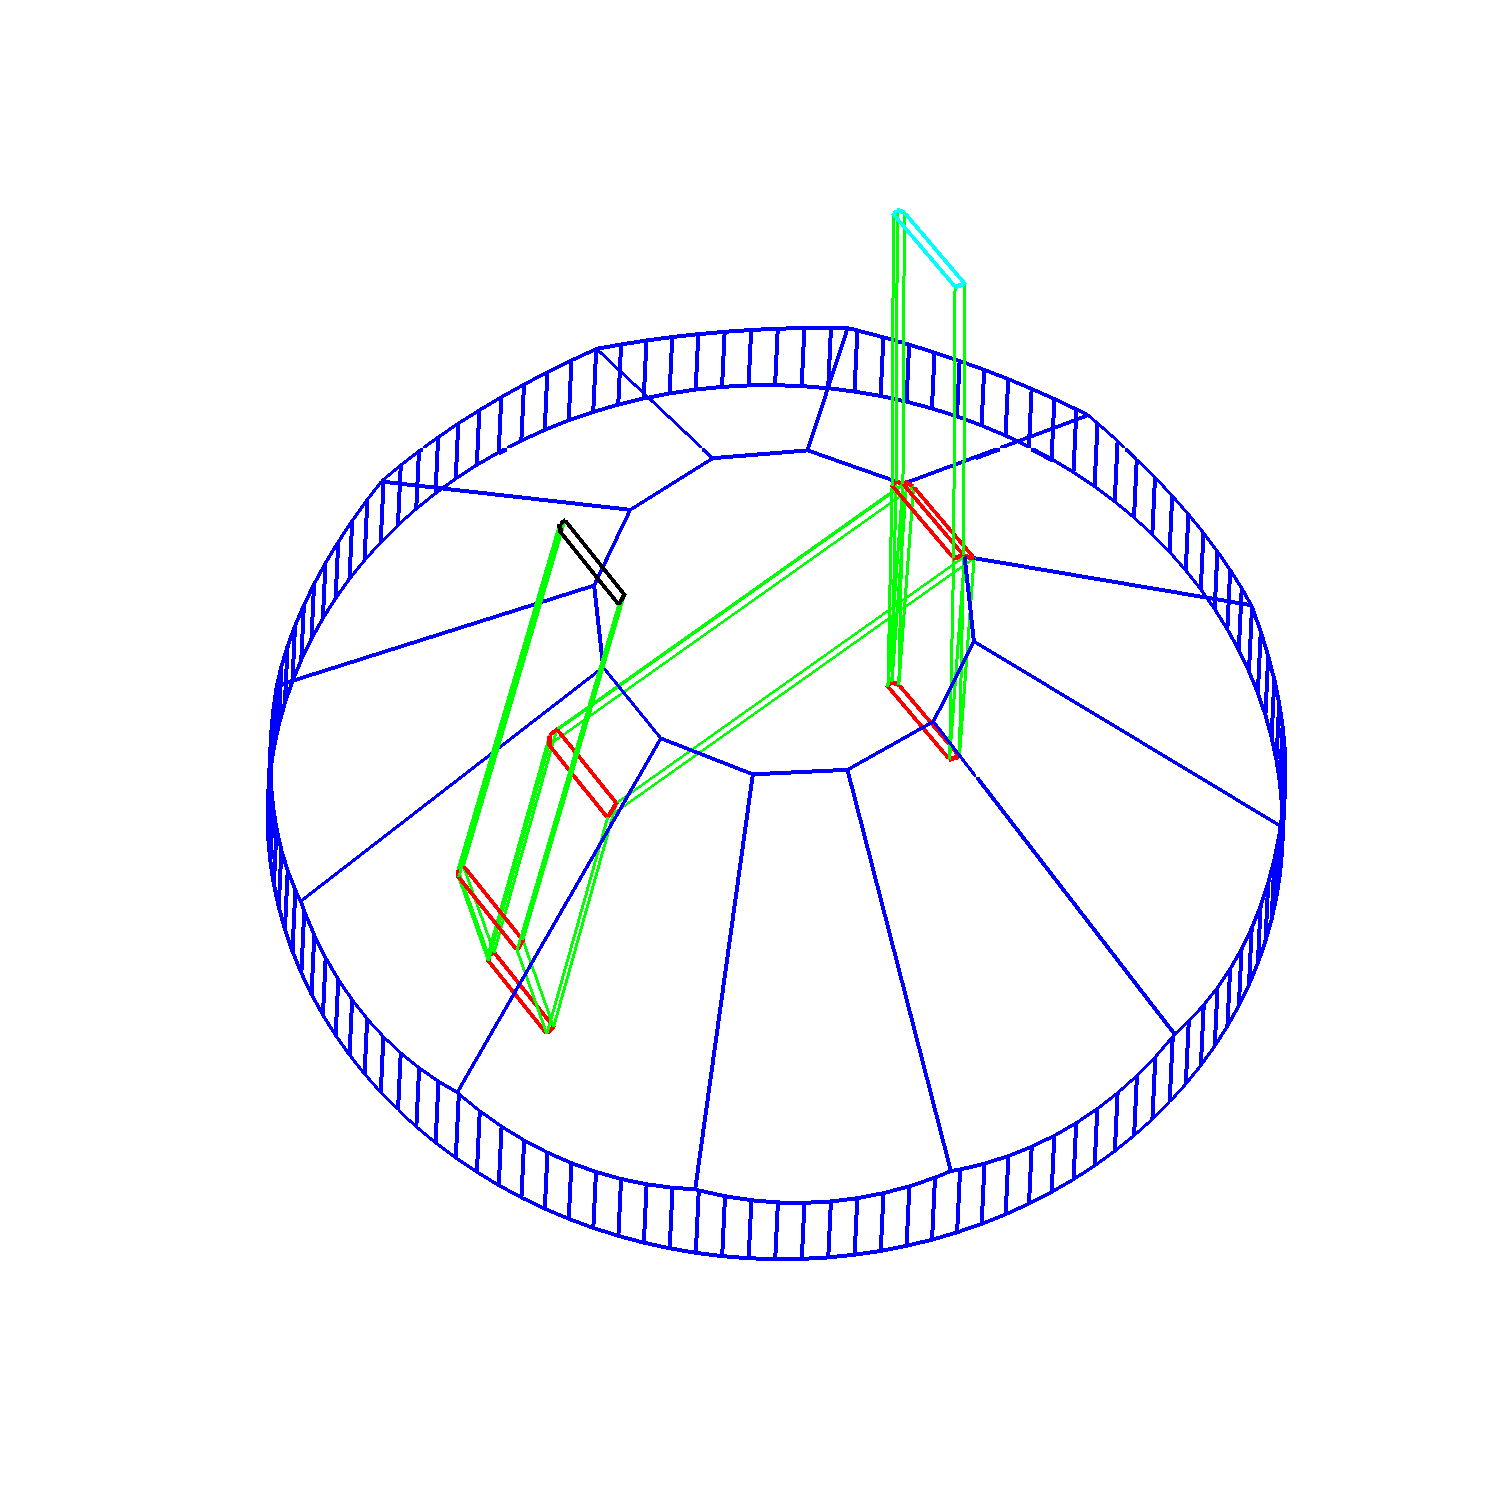
\includegraphics[width=\textwidth]{group6E.pdf}
\end{minipage}
\begin{minipage}[c]{0.325\textwidth}
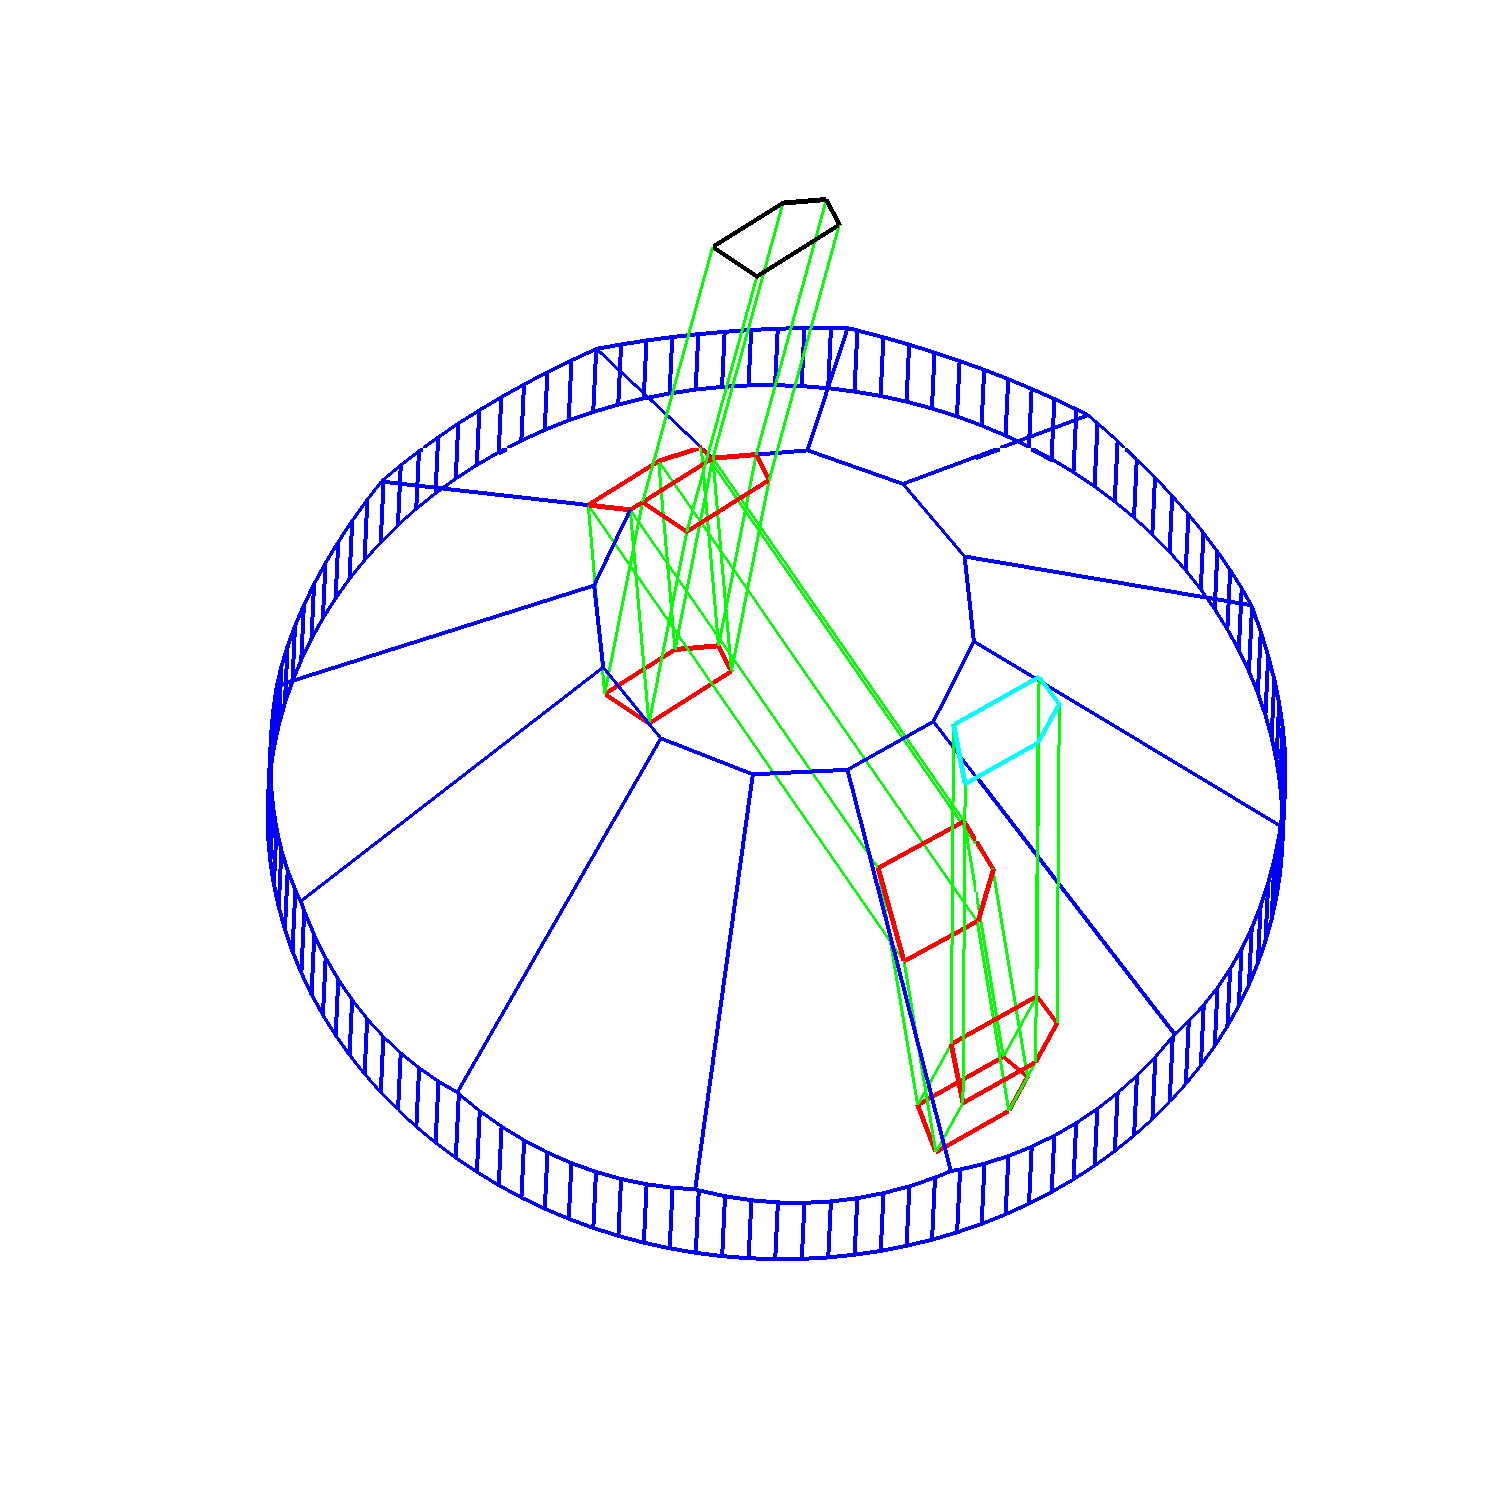
\includegraphics[width=\textwidth]{group6F.pdf}
\end{minipage}\\

\begin{minipage}[c]{0.325\textwidth}
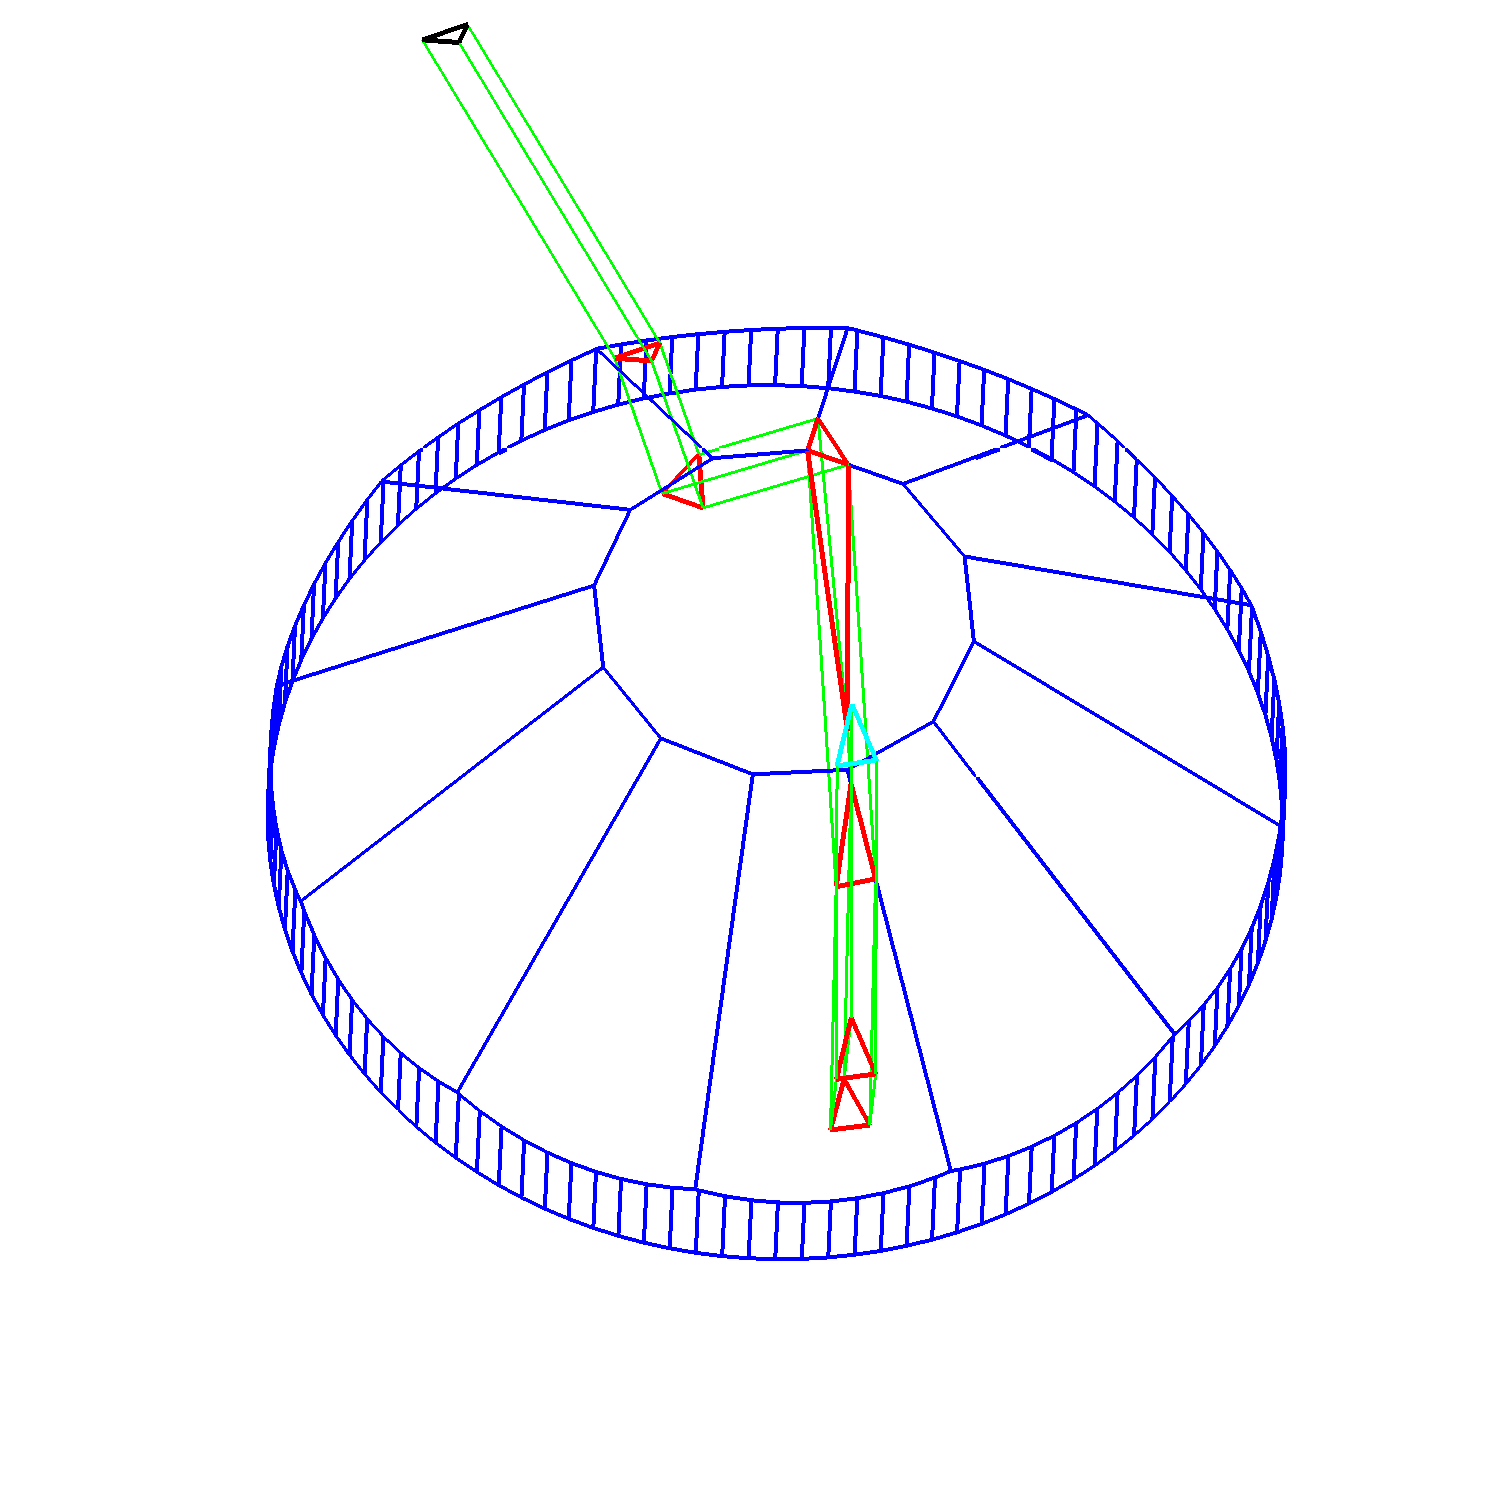
\includegraphics[width=\textwidth]{group7A.pdf}
\end{minipage}
\begin{minipage}[c]{0.325\textwidth}
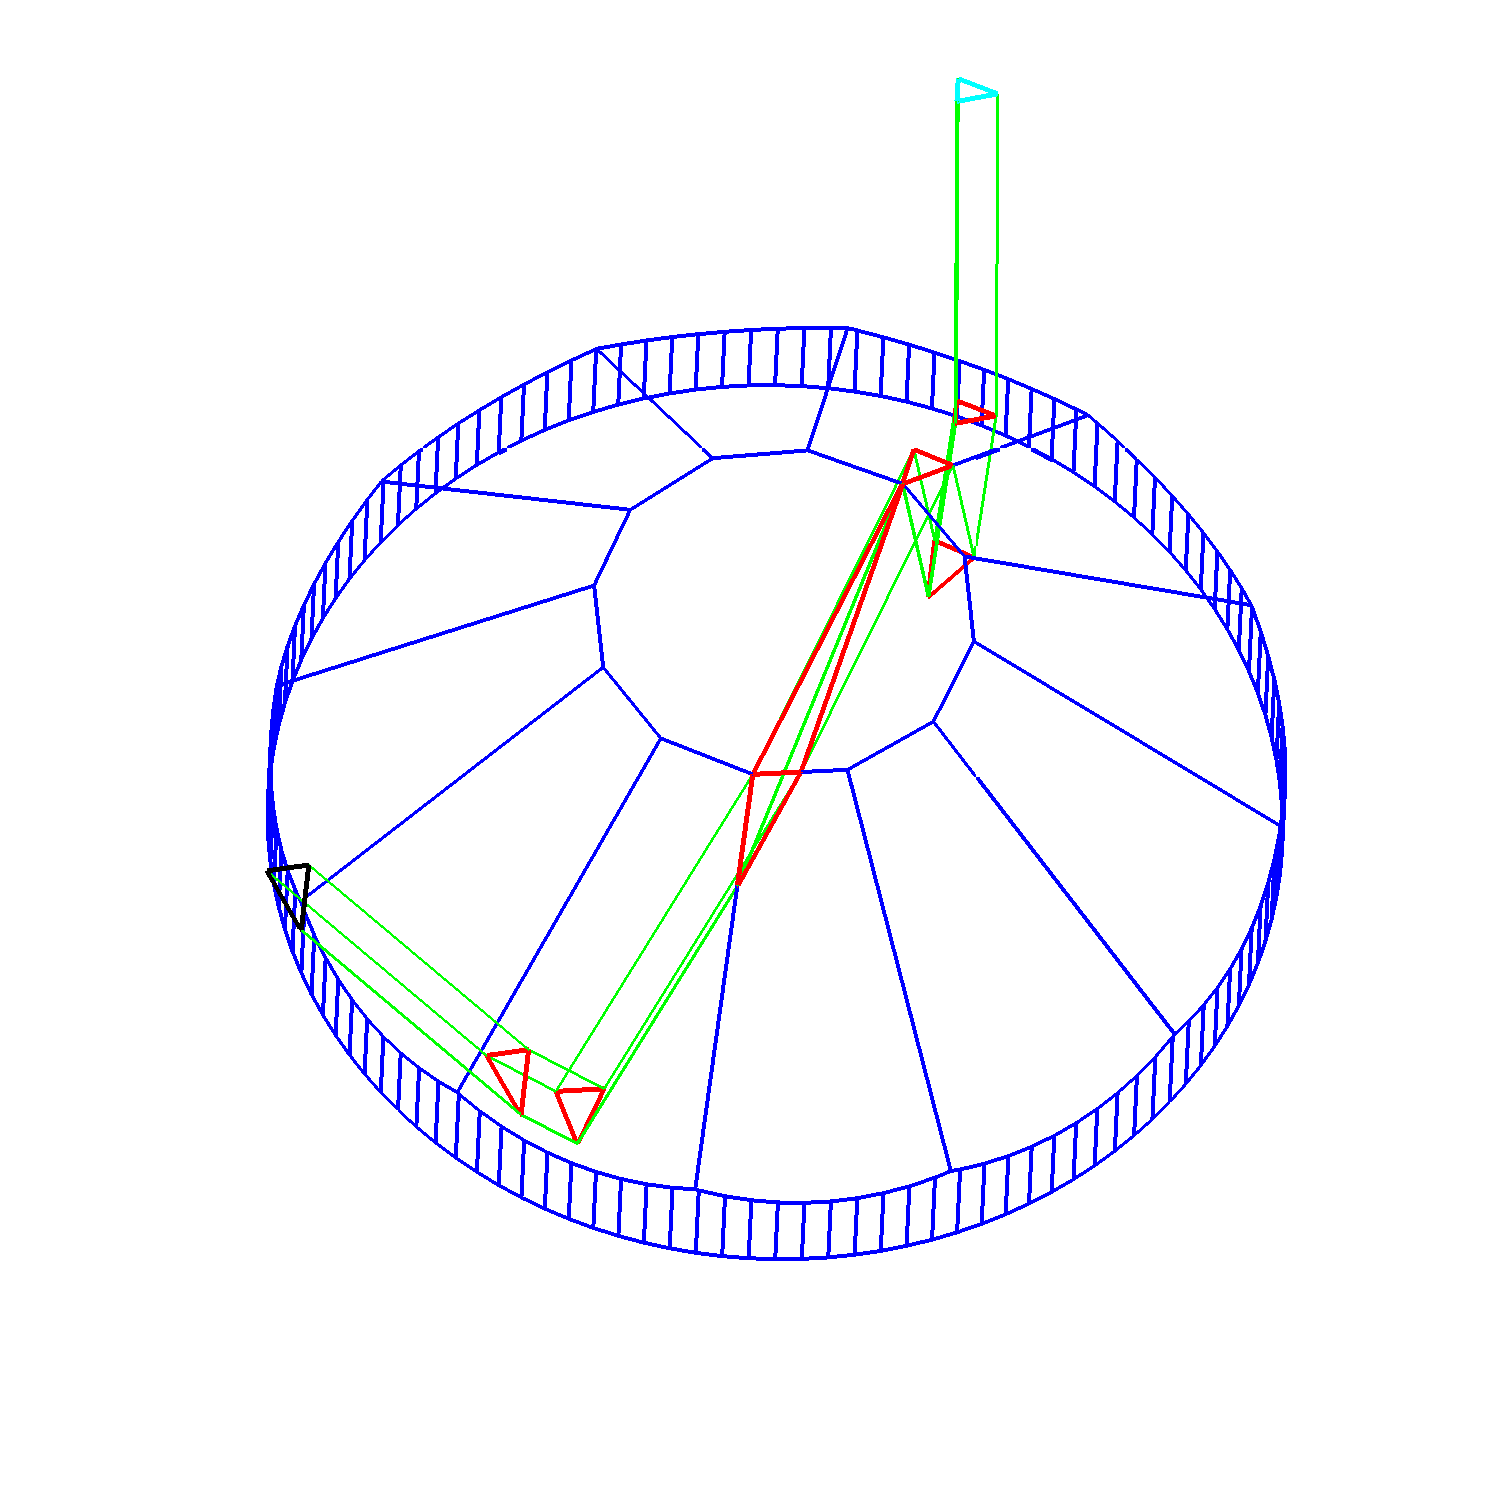
\includegraphics[width=\textwidth]{group7B.pdf}
\end{minipage}
\begin{minipage}[c]{0.325\textwidth}
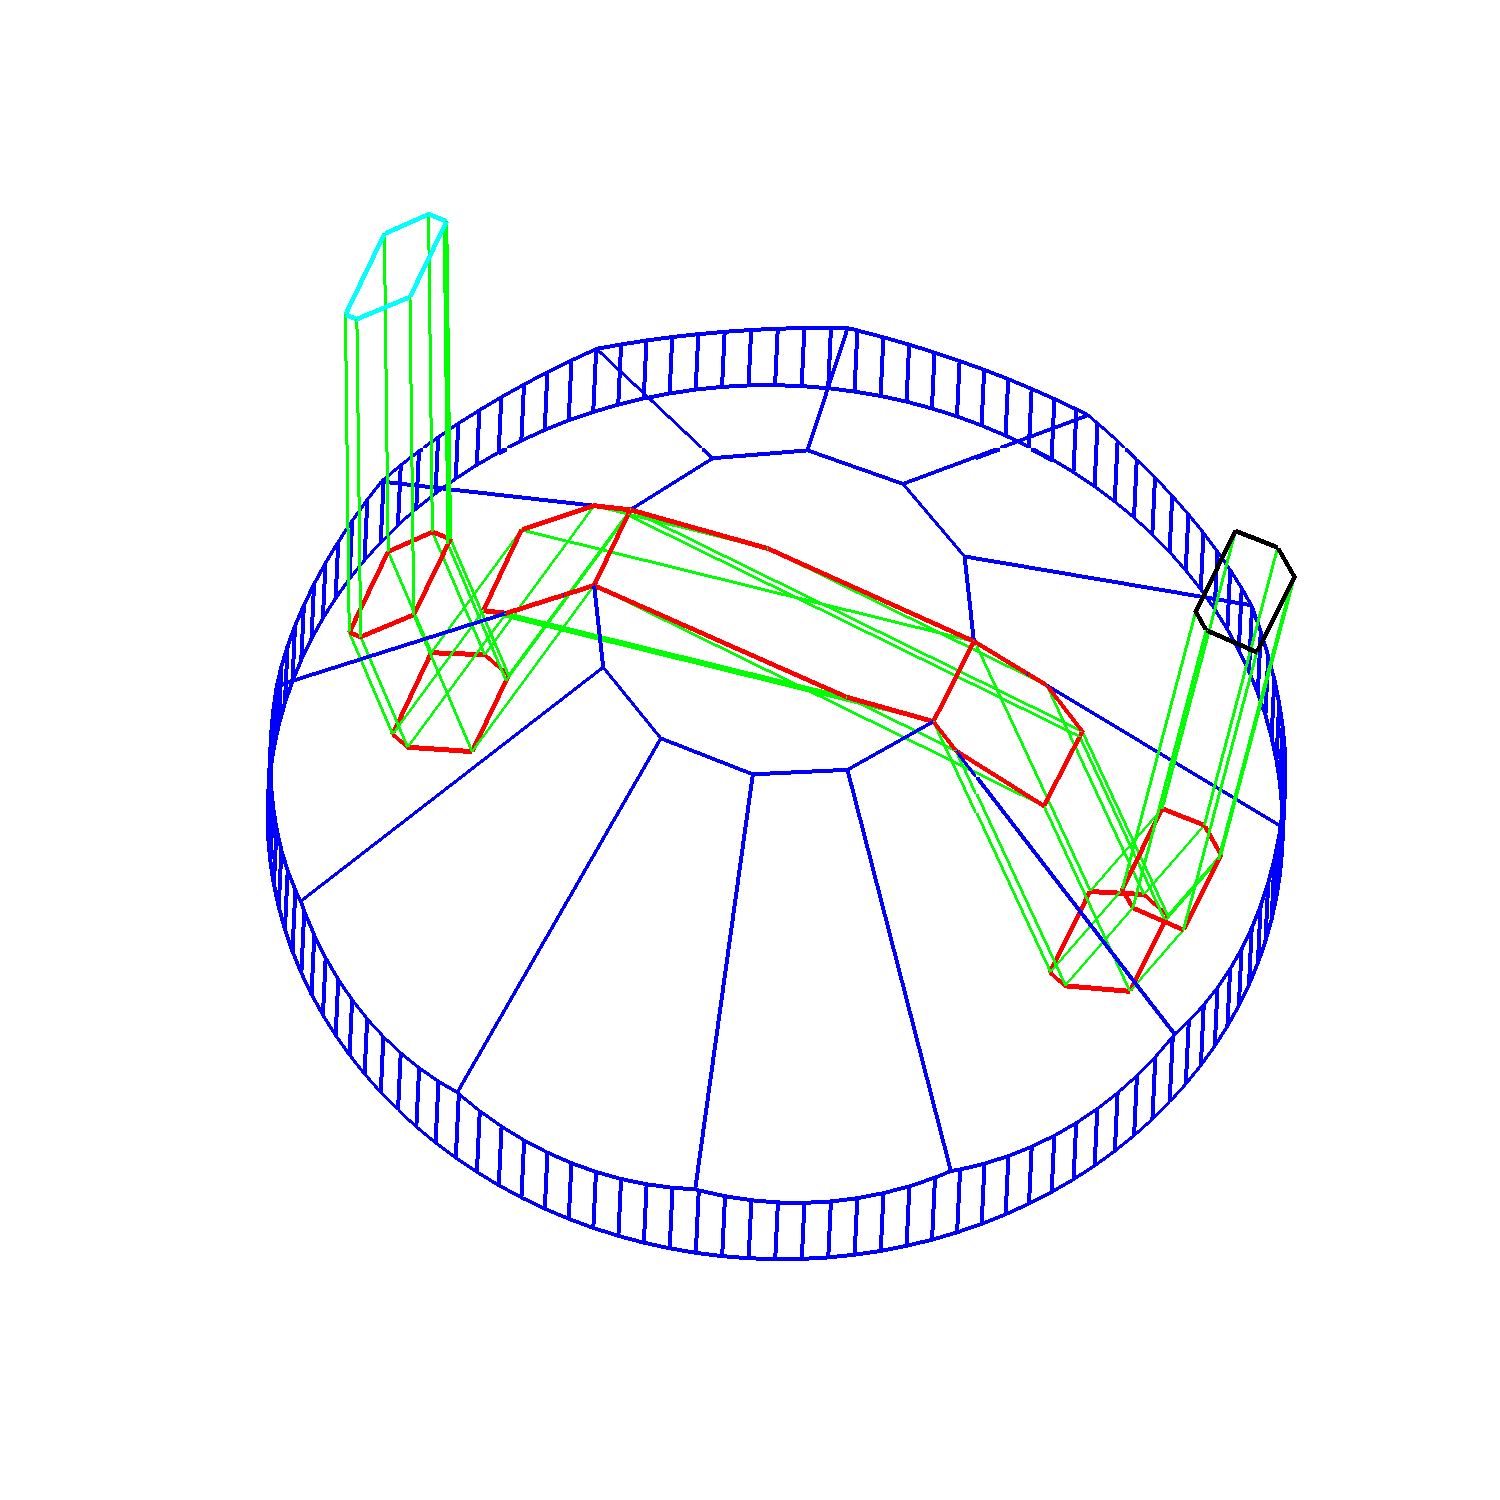
\includegraphics[width=\textwidth]{group7C.pdf}
\end{minipage}\\

\begin{minipage}[c]{0.325\textwidth}
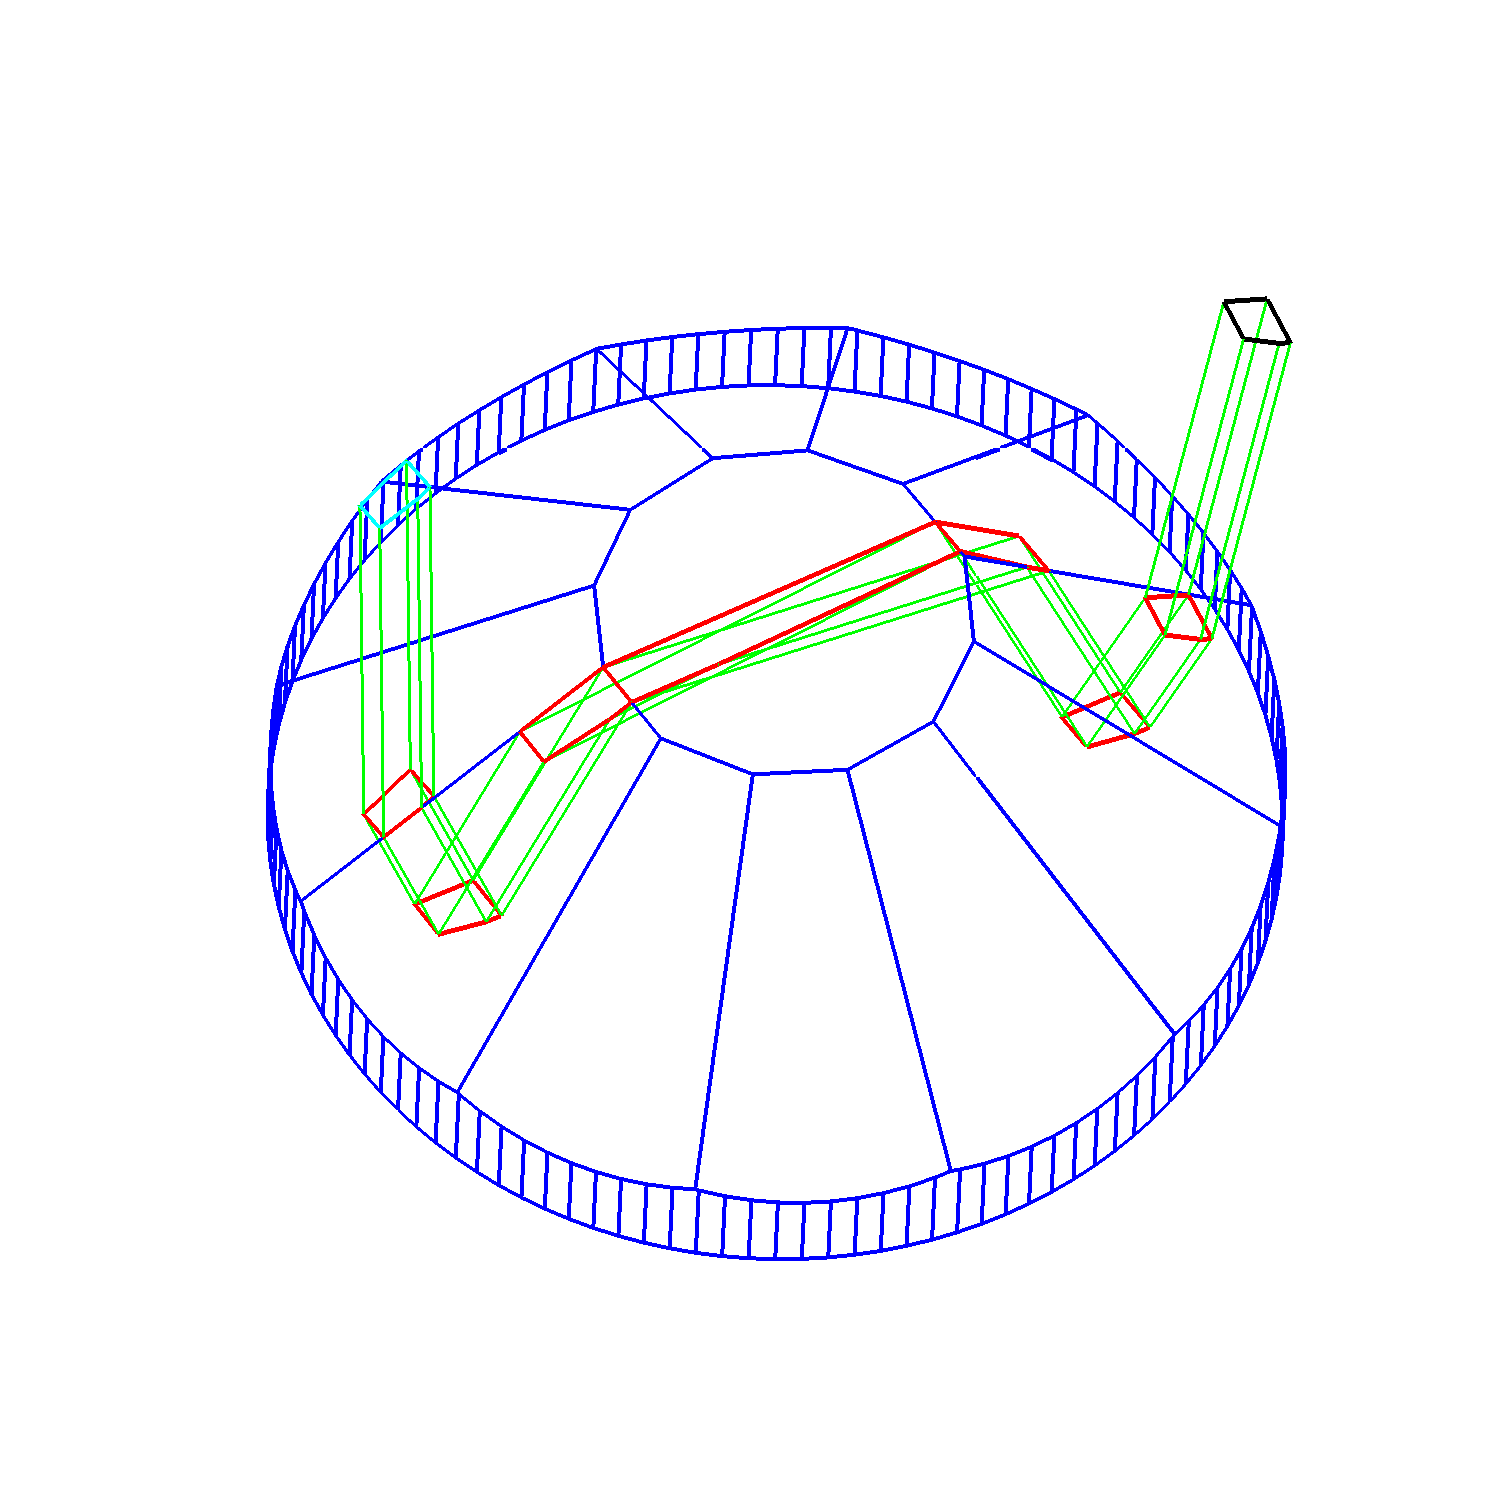
\includegraphics[width=\textwidth]{group7D.pdf}
\end{minipage}
\begin{minipage}[c]{0.325\textwidth}
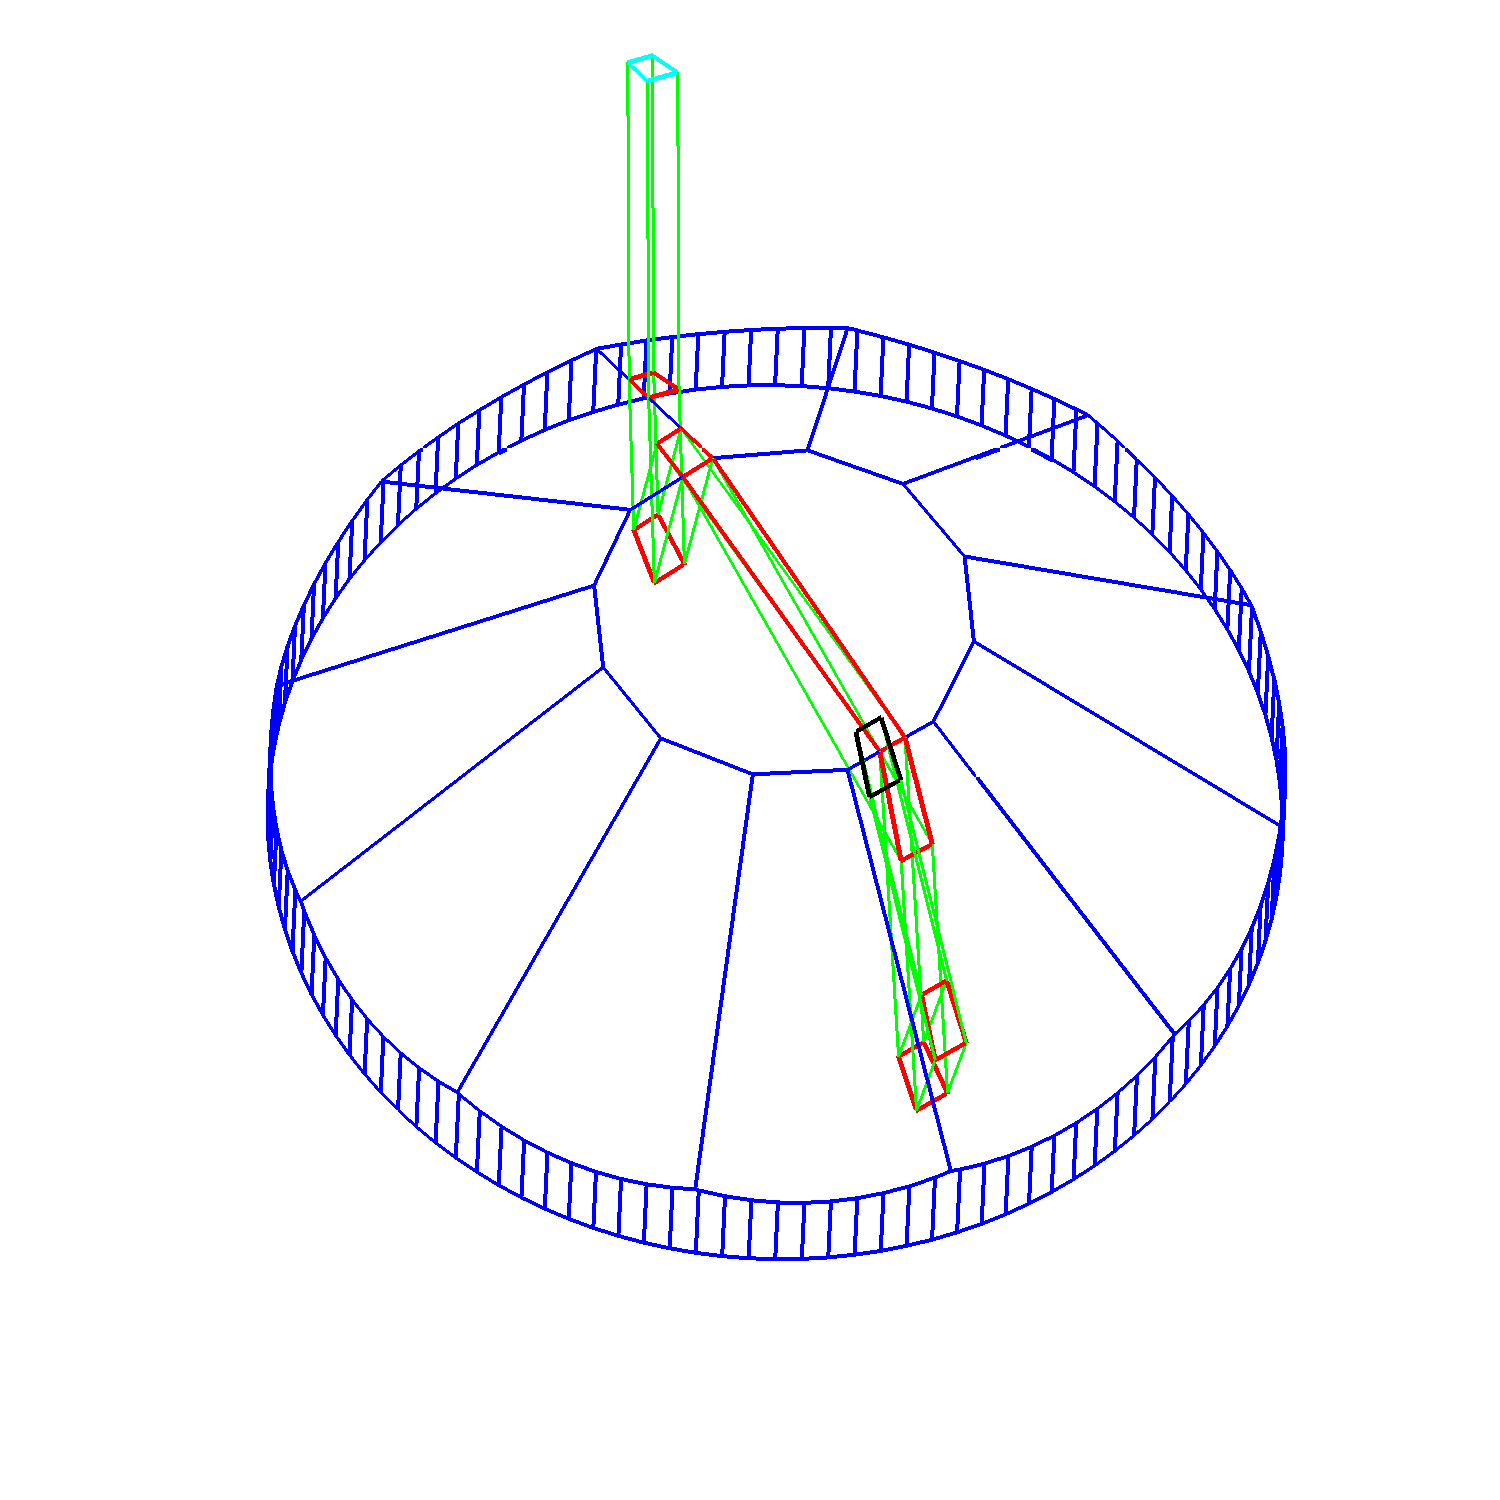
\includegraphics[width=\textwidth]{group7E.pdf}
\end{minipage}
\begin{minipage}[c]{0.325\textwidth}
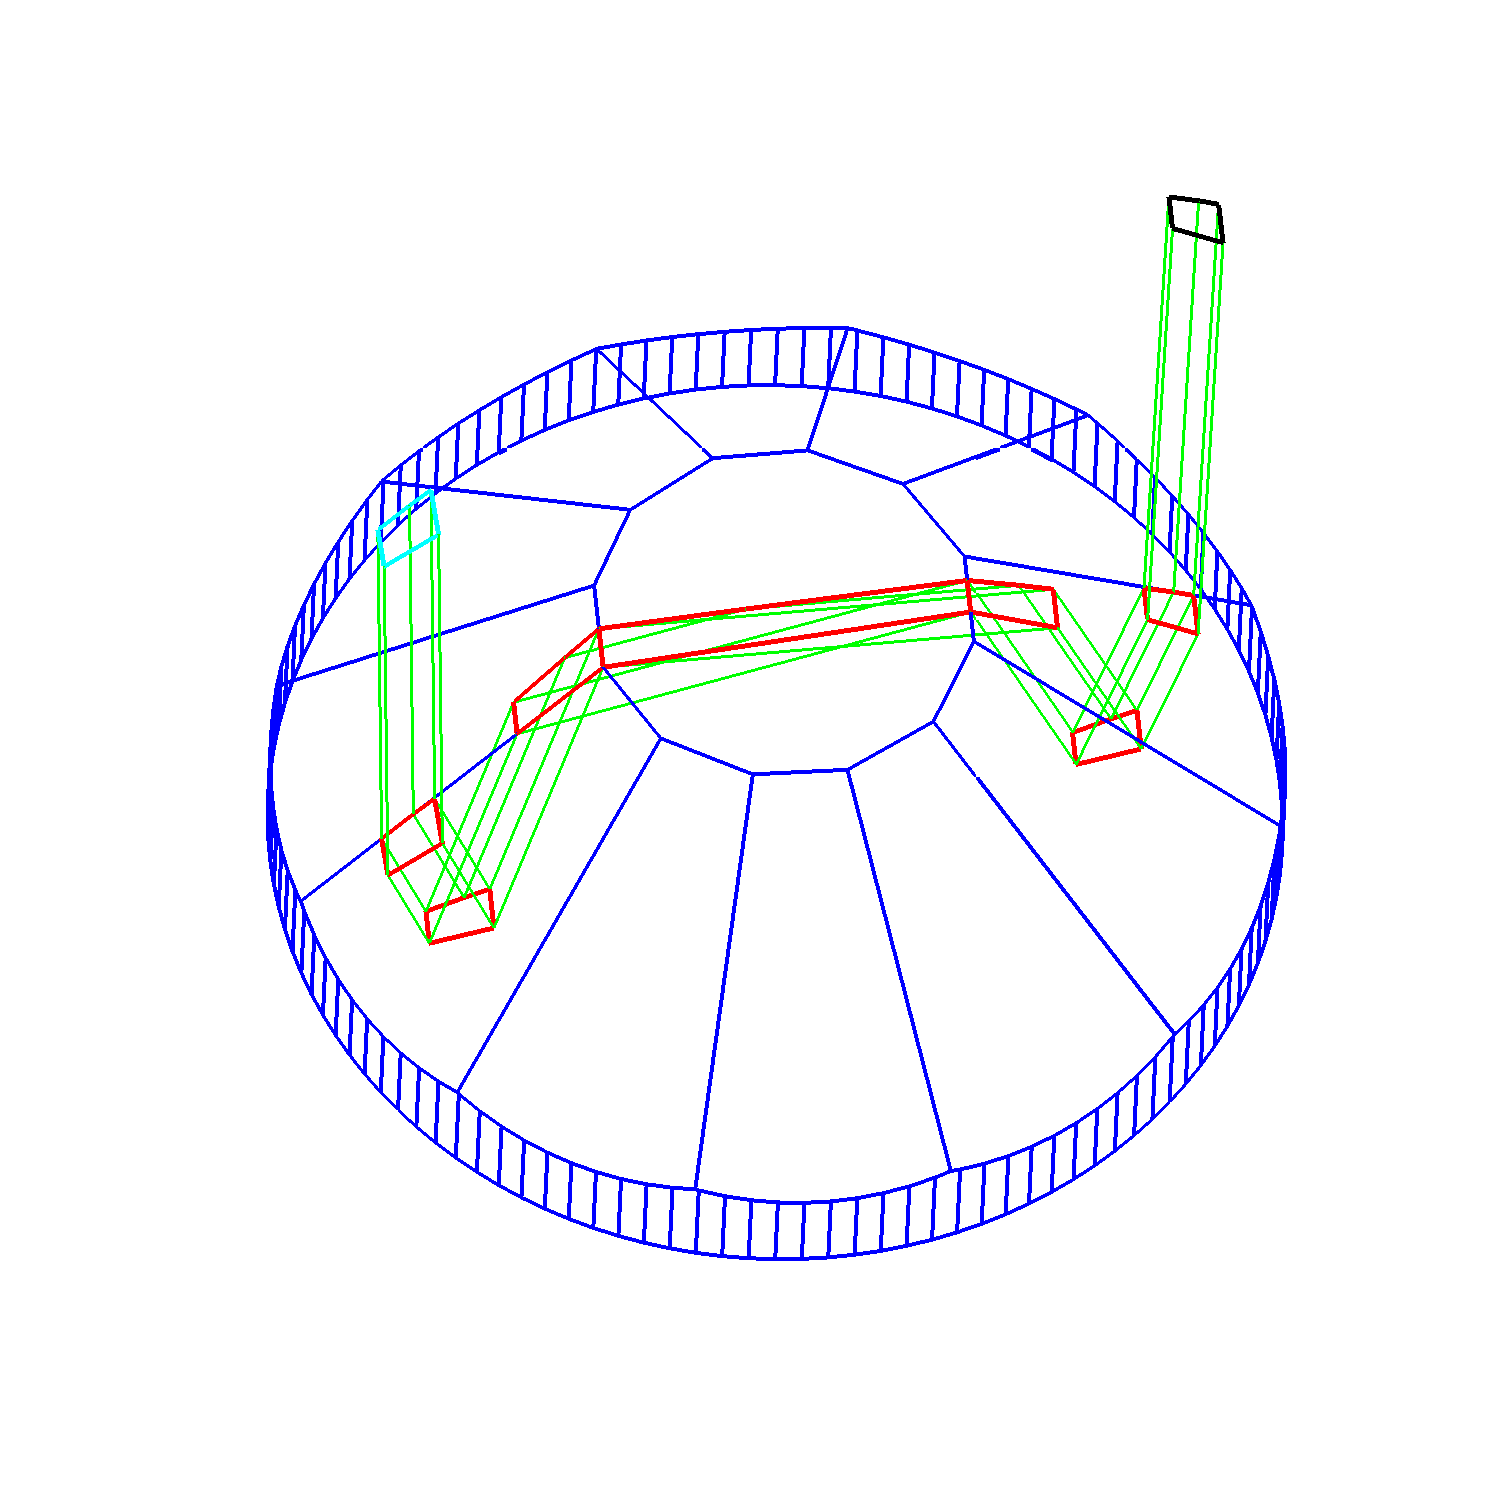
\includegraphics[width=\textwidth]{group7F.pdf}
\end{minipage}\\

\begin{minipage}[c]{0.325\textwidth}
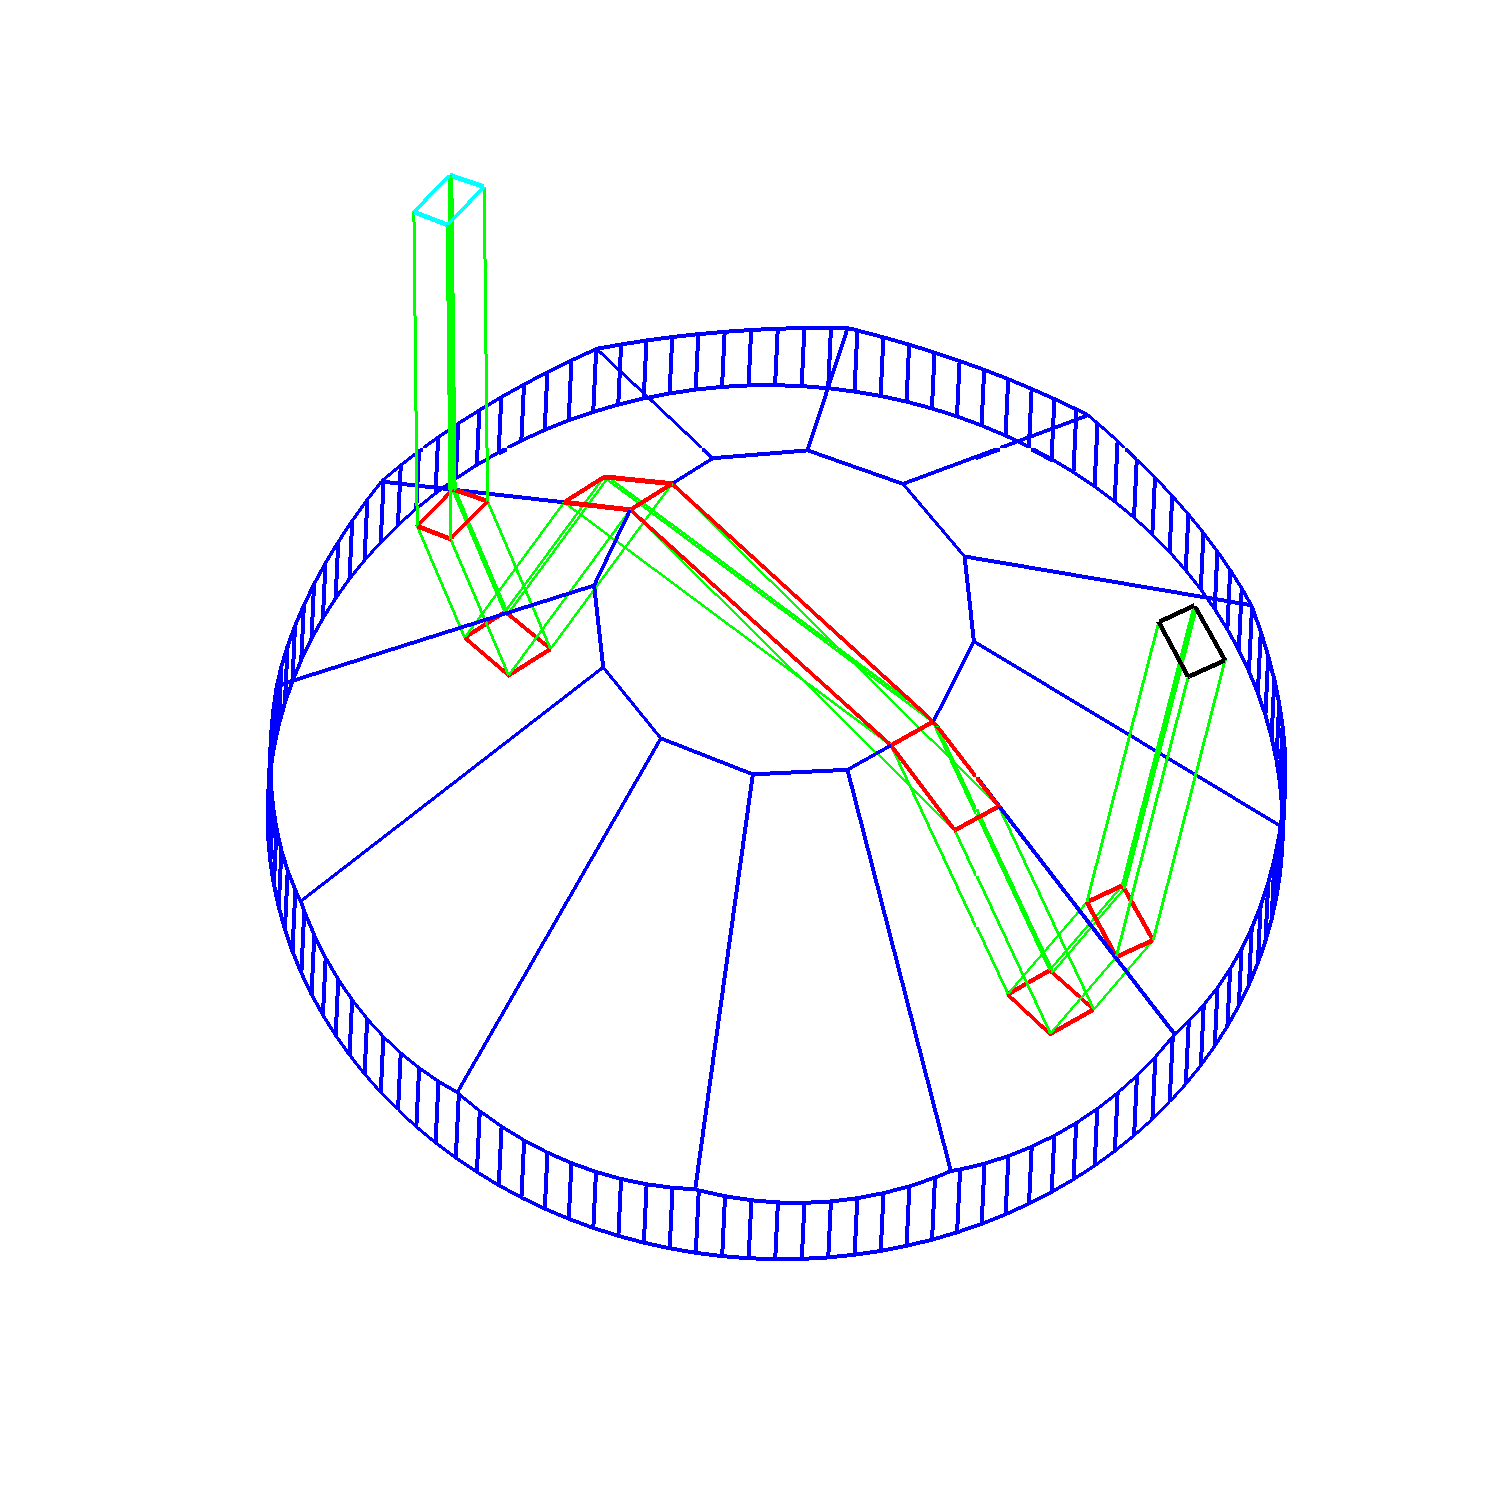
\includegraphics[width=\textwidth]{group7G.pdf}
\end{minipage}
\begin{minipage}[c]{0.325\textwidth}
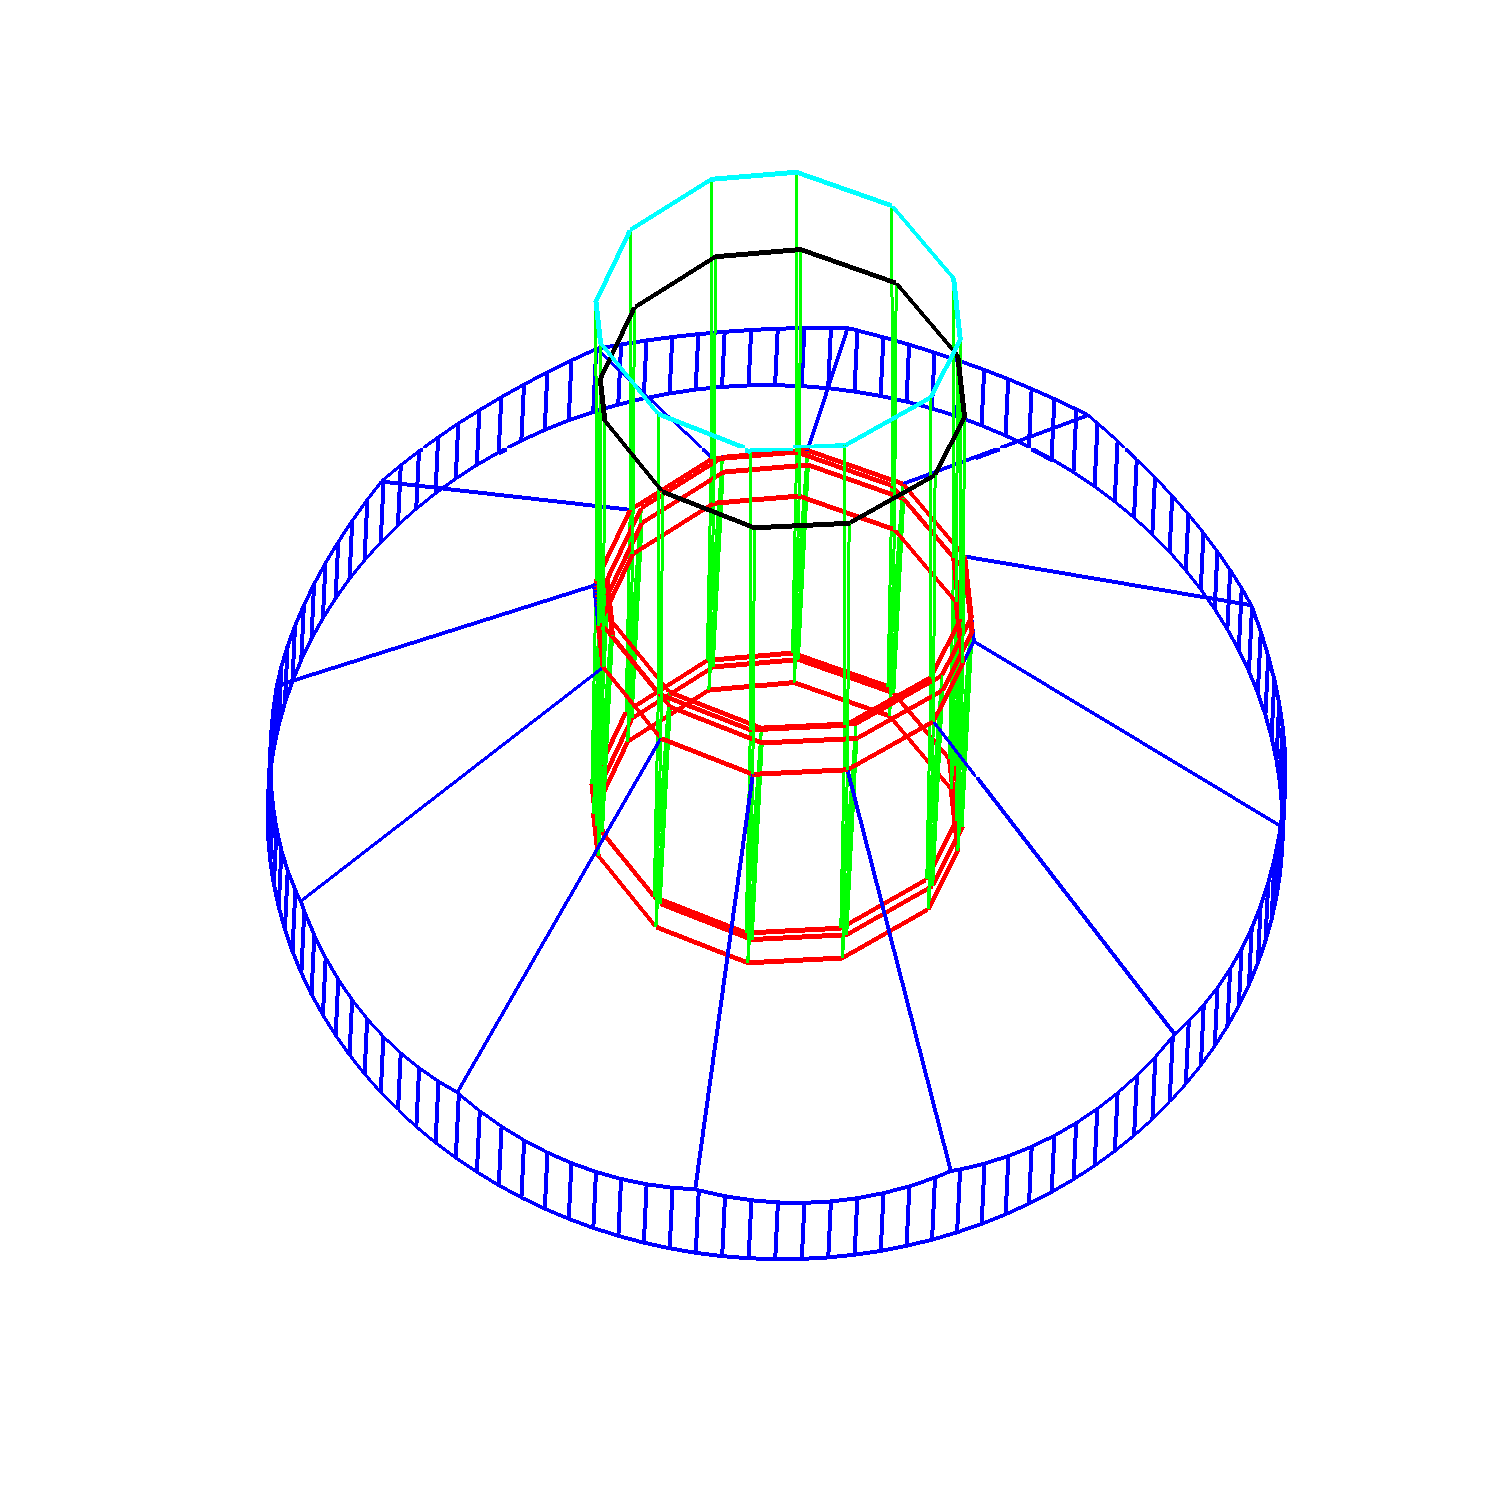
\includegraphics[width=\textwidth]{group7H.pdf}
\end{minipage}
\begin{minipage}[c]{0.325\textwidth}
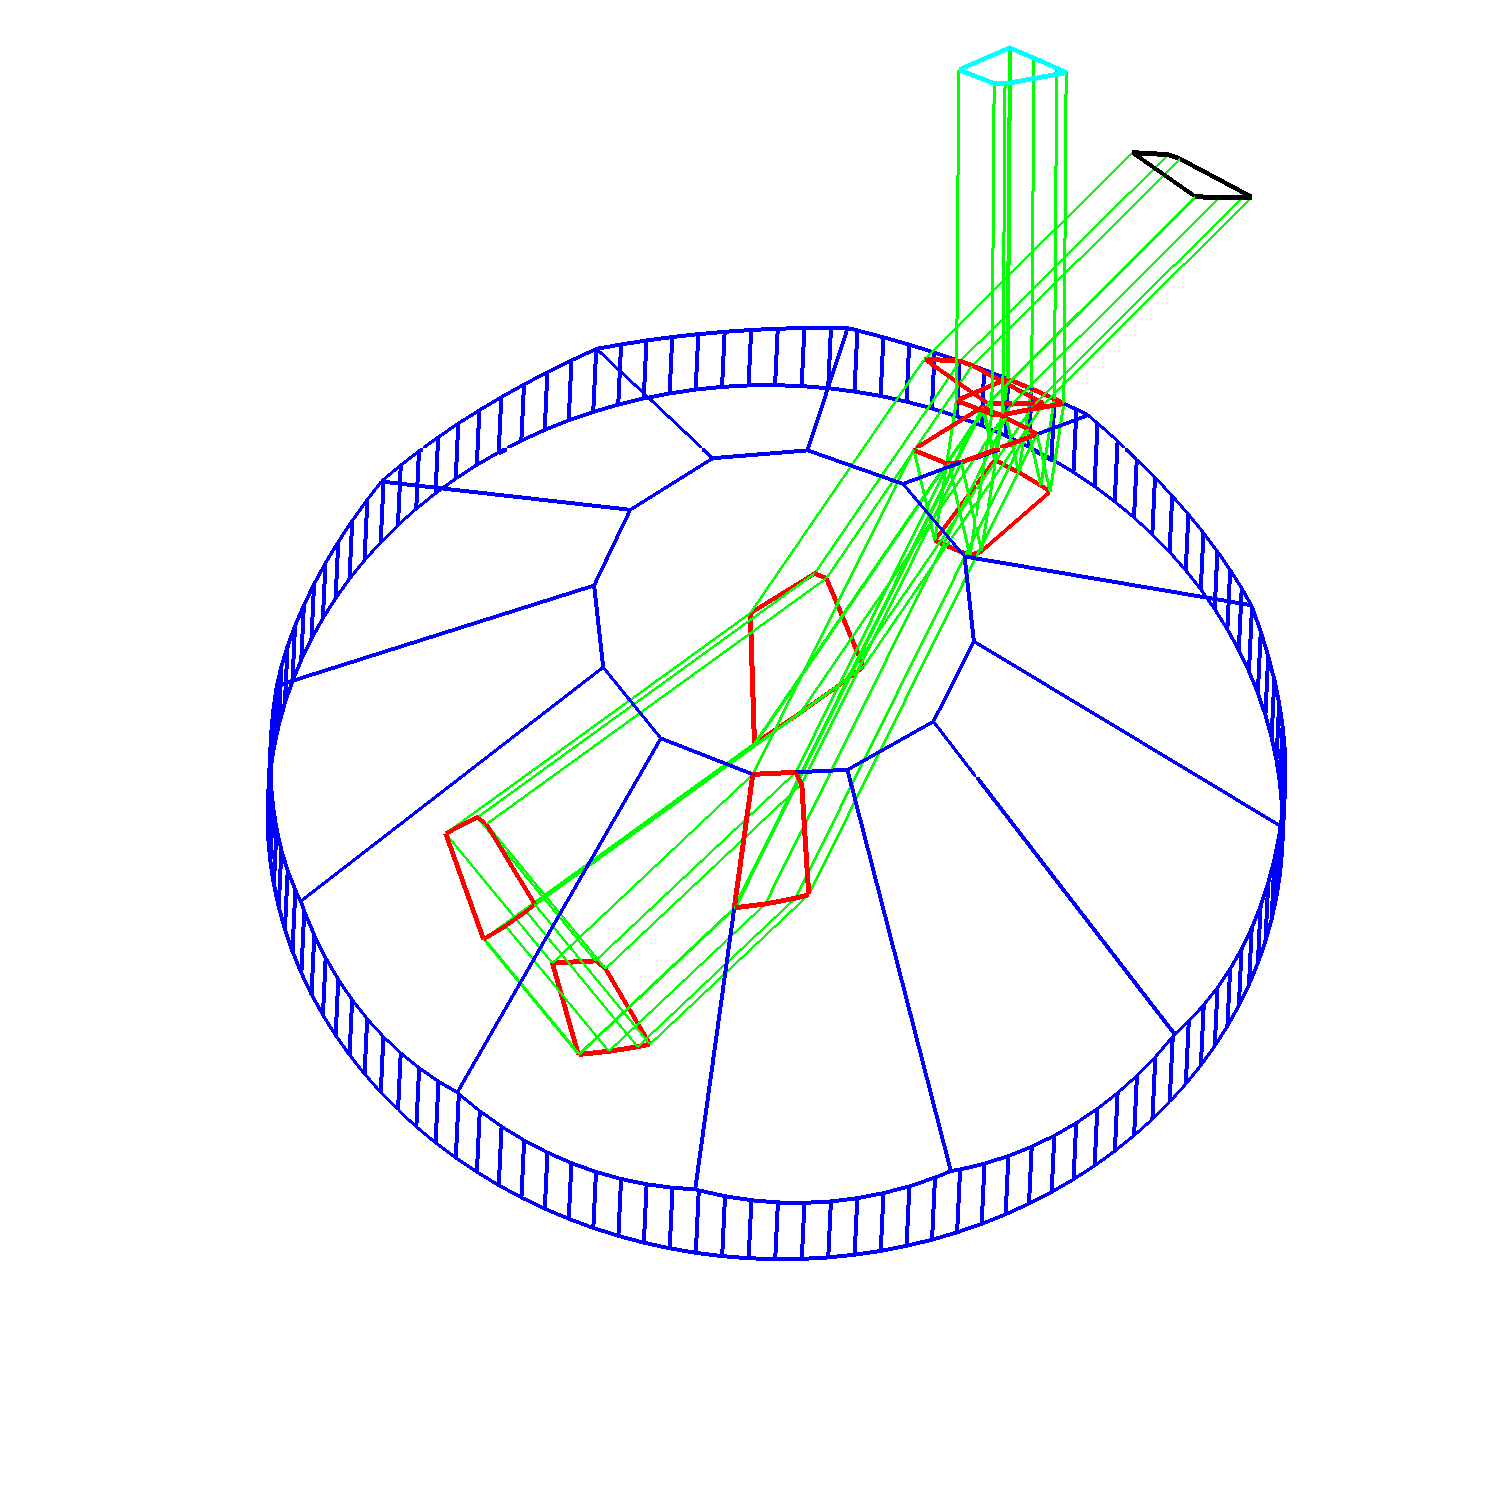
\includegraphics[width=\textwidth]{group8A.pdf}
\end{minipage}

\caption{3D view of ray example in classes 6D, 6E, 6F, 7A, 7B, 7C, 7D, 7E, 7F, 7G, 7H, 8A.}
\label{fig:modelClass3D1}
\end{figure}


\begin{figure}[htps]
\centering
\begin{minipage}[c]{0.325\textwidth}
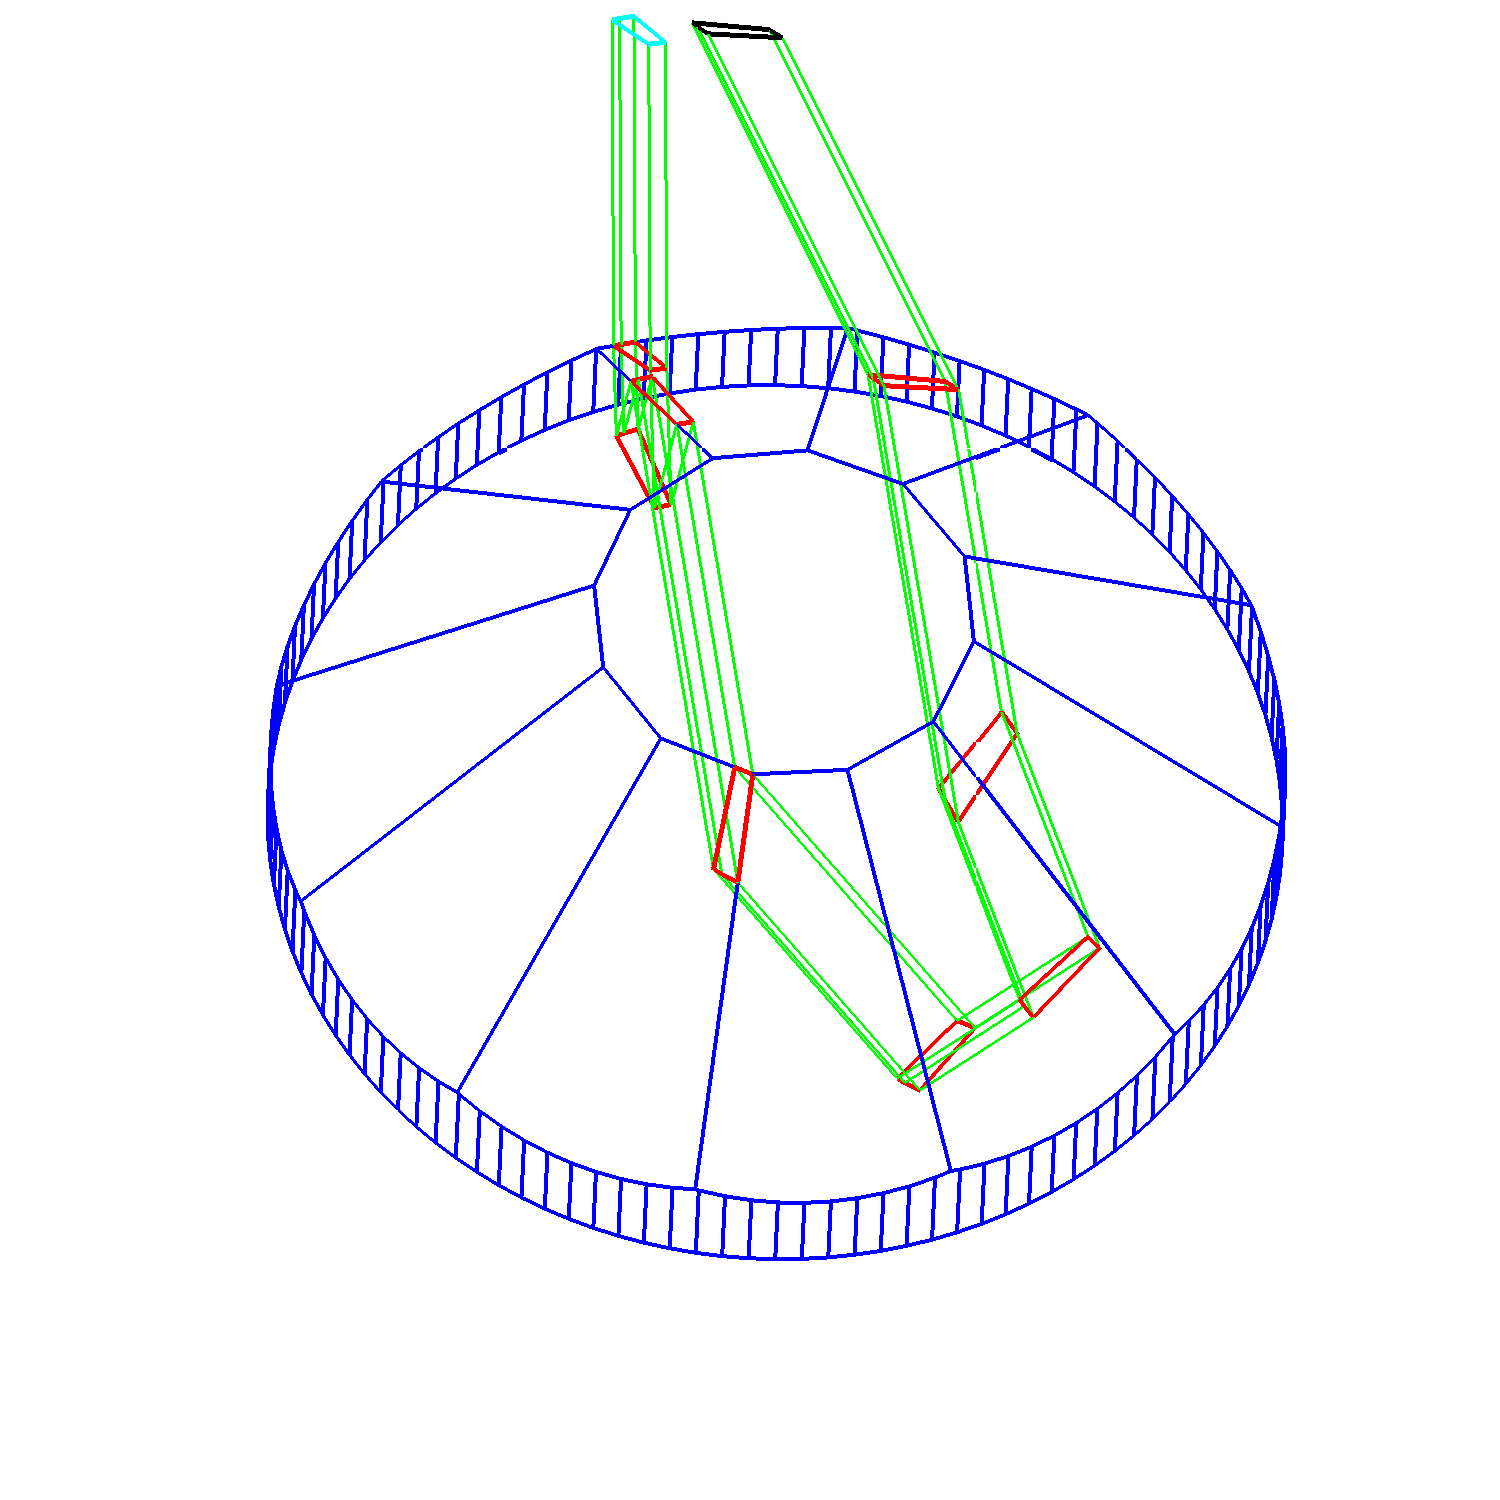
\includegraphics[width=\textwidth]{group8B.pdf}
\end{minipage}
\begin{minipage}[c]{0.325\textwidth}
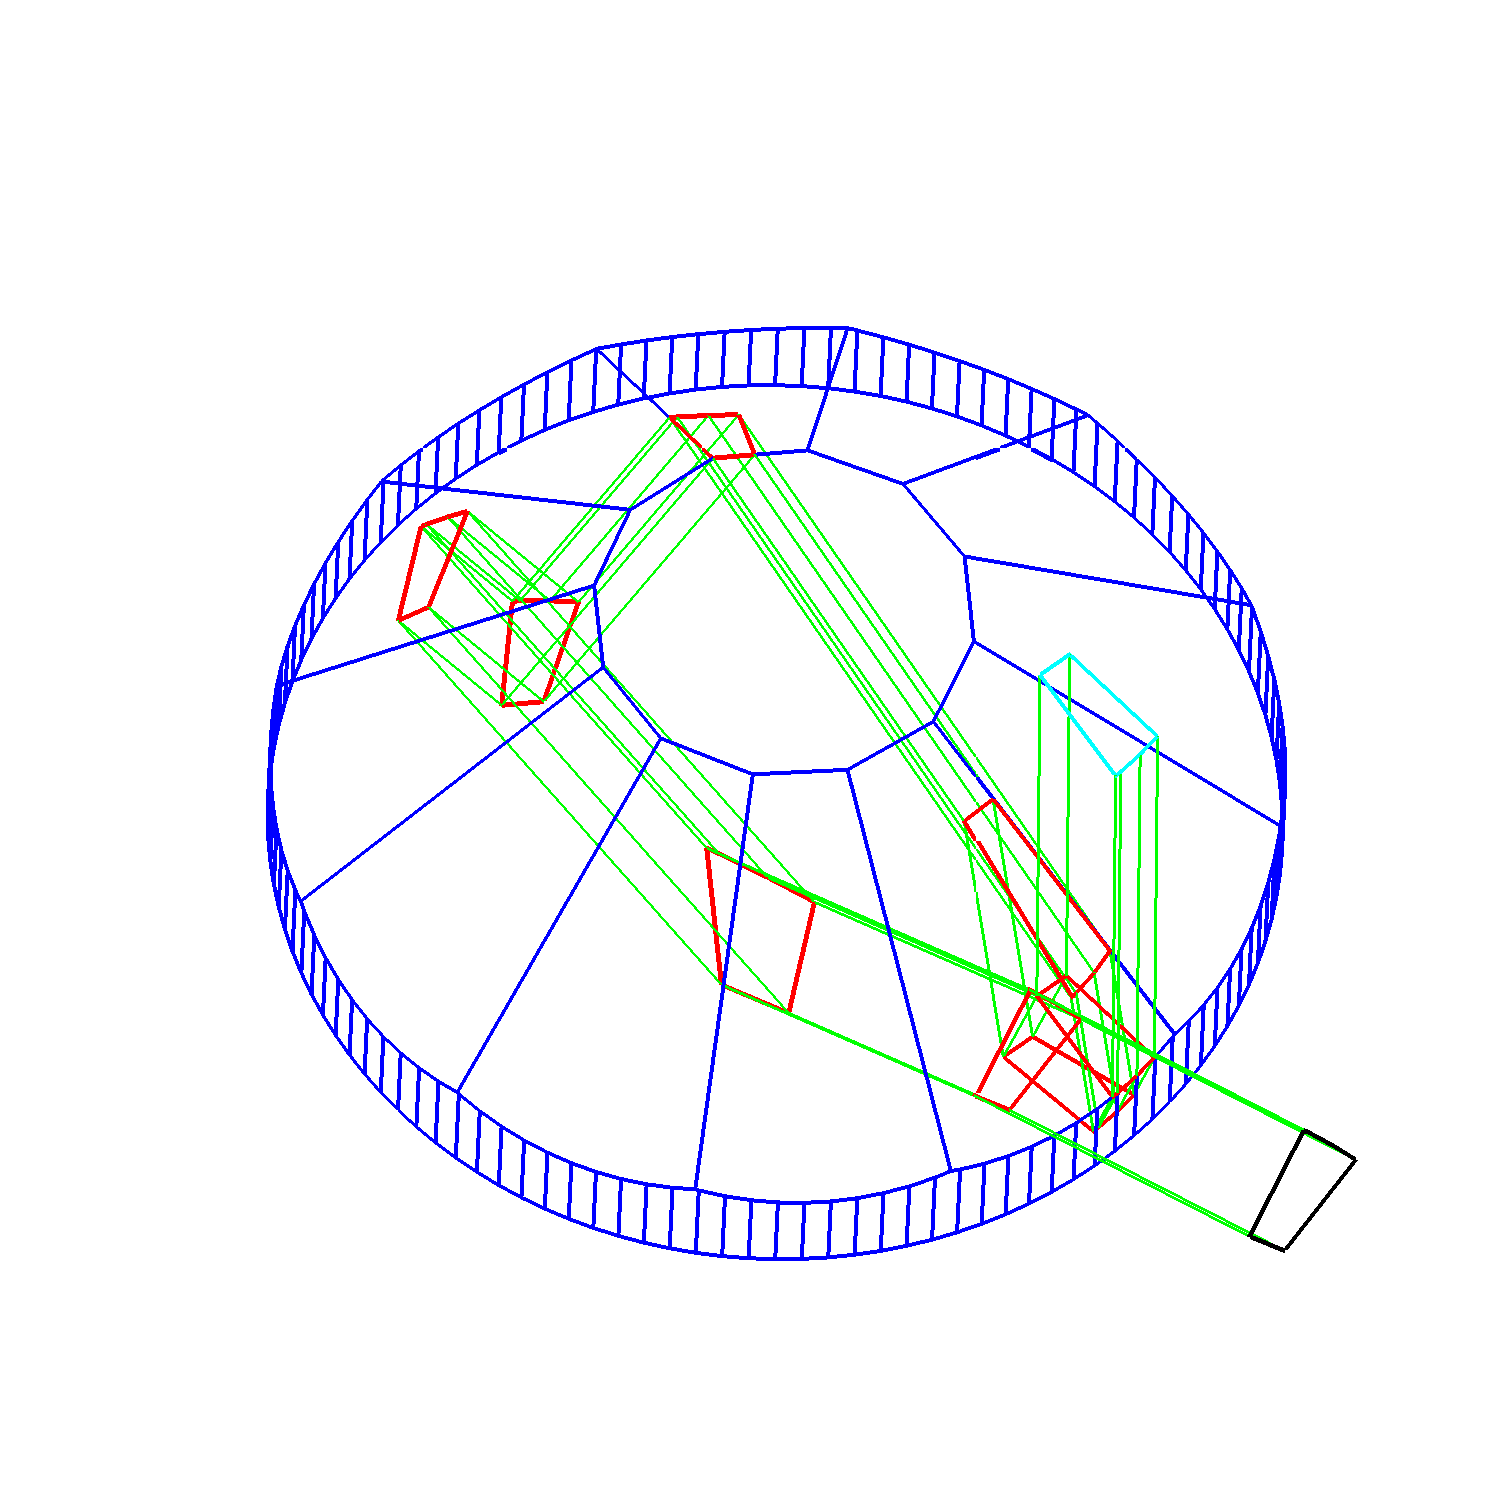
\includegraphics[width=\textwidth]{group8C.pdf}
\end{minipage}
\begin{minipage}[c]{0.325\textwidth}
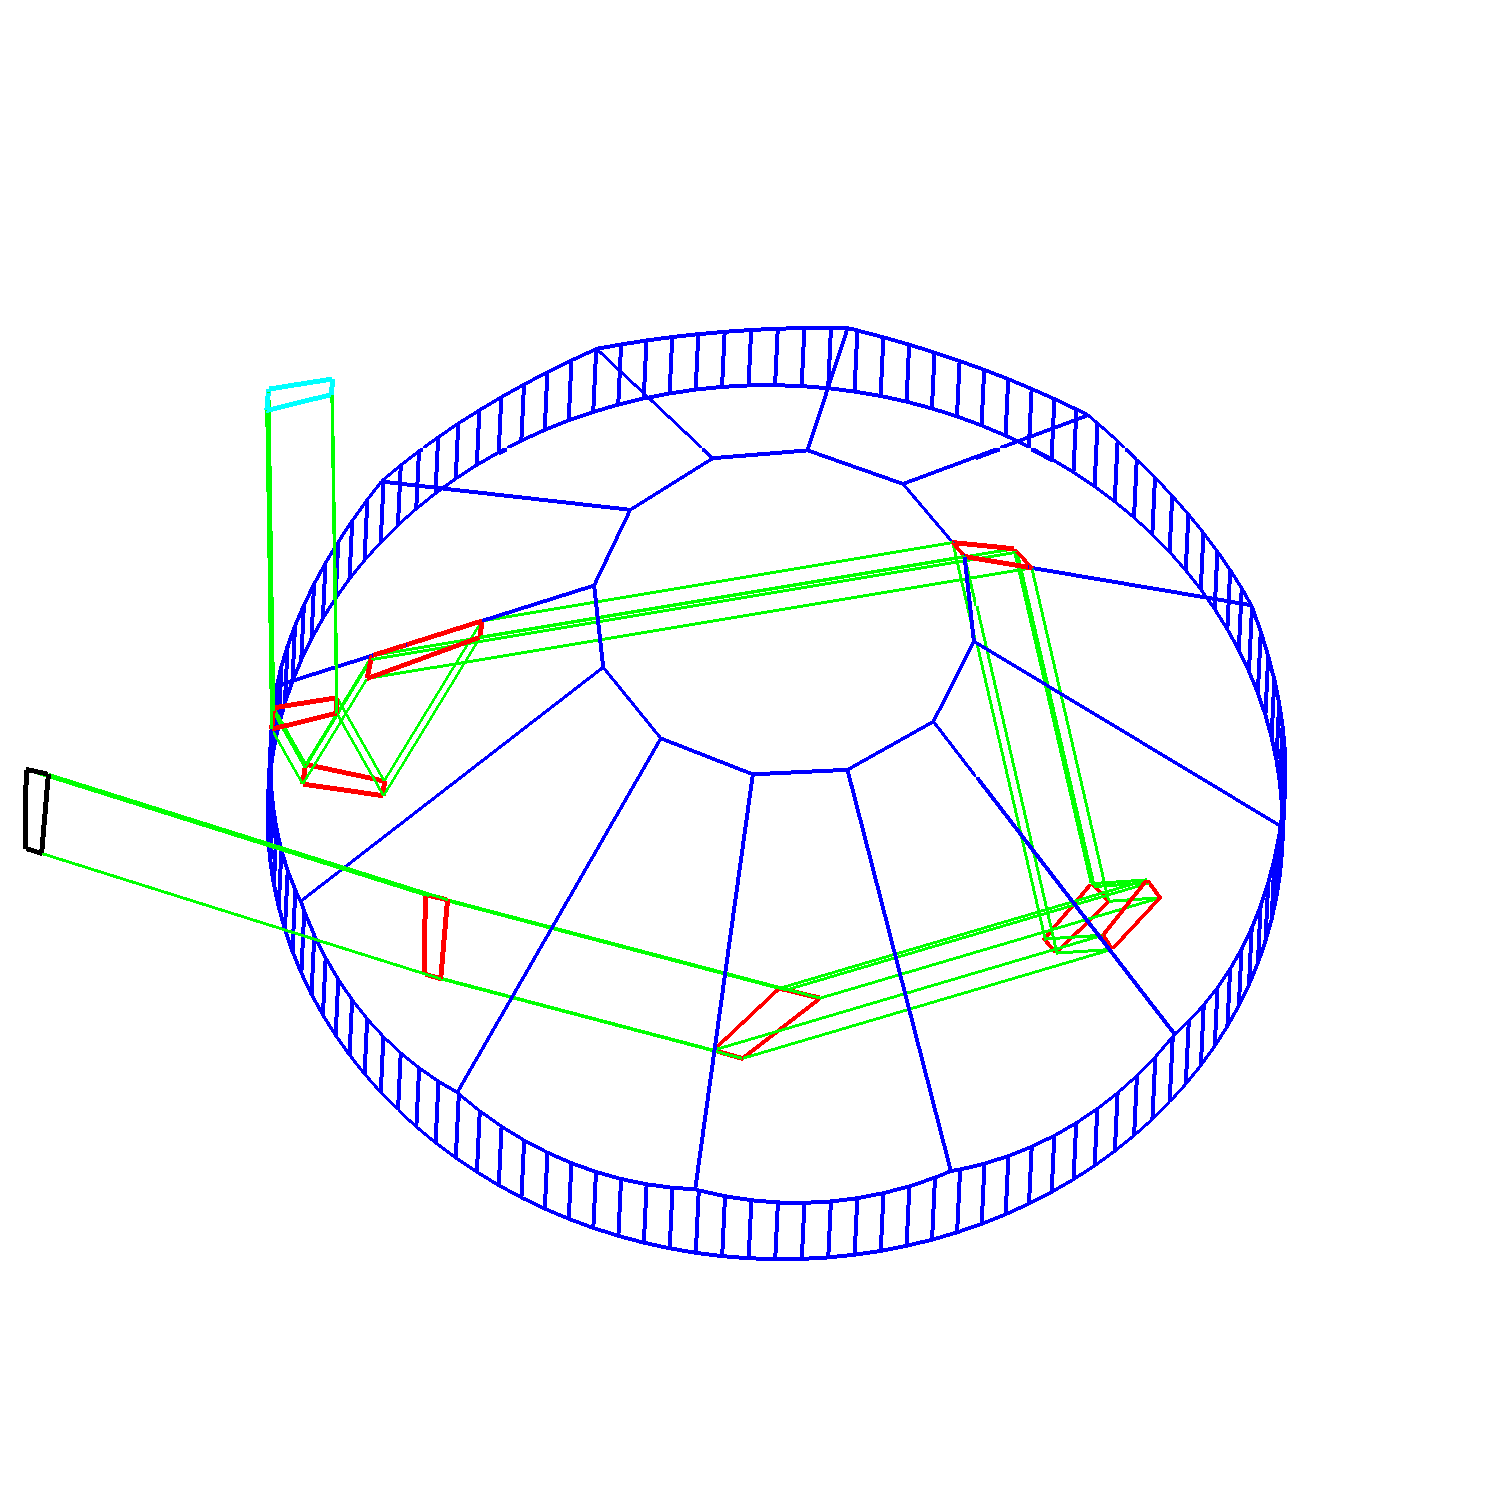
\includegraphics[width=\textwidth]{group8D.pdf}
\end{minipage}\\

\begin{minipage}[c]{0.325\textwidth}
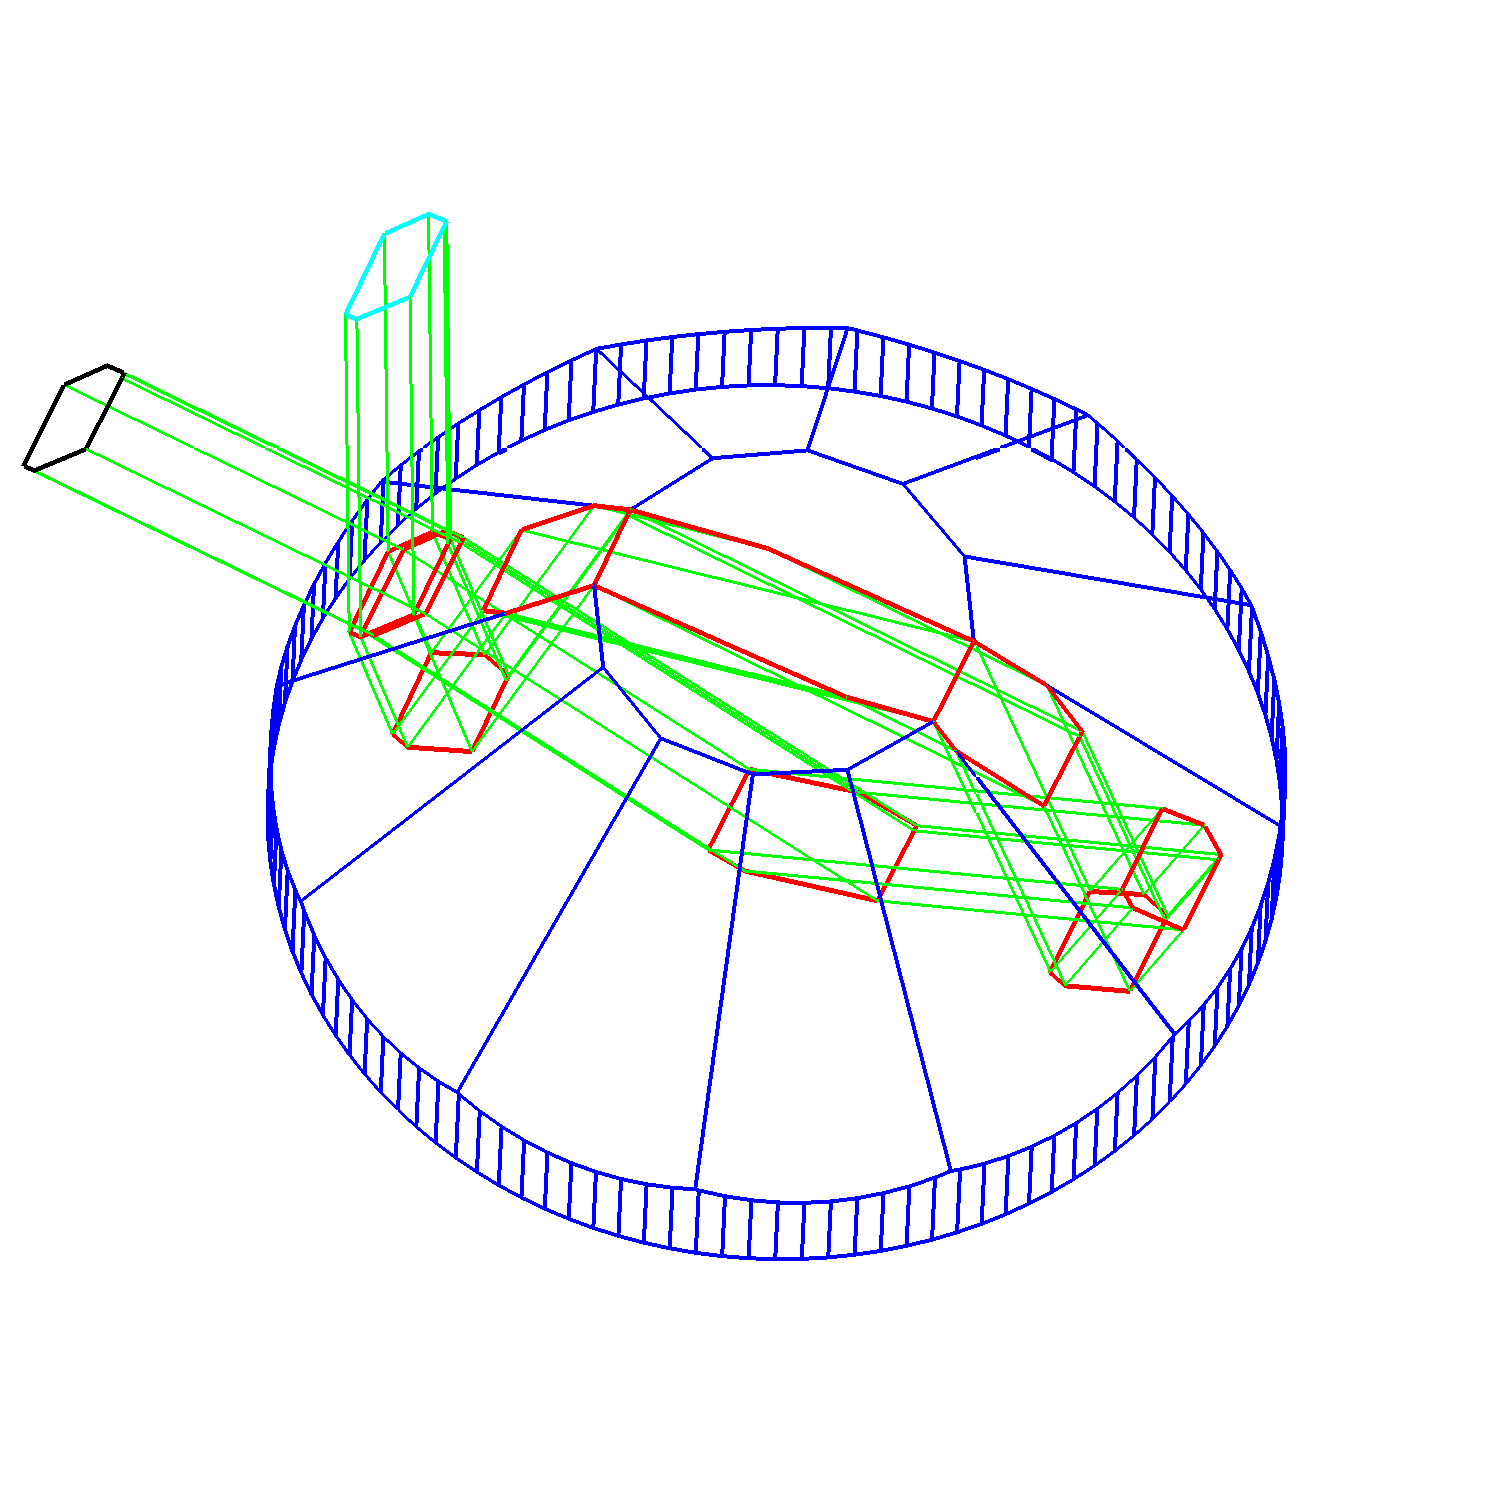
\includegraphics[width=\textwidth]{group9A.pdf}
\end{minipage}
\begin{minipage}[c]{0.325\textwidth}
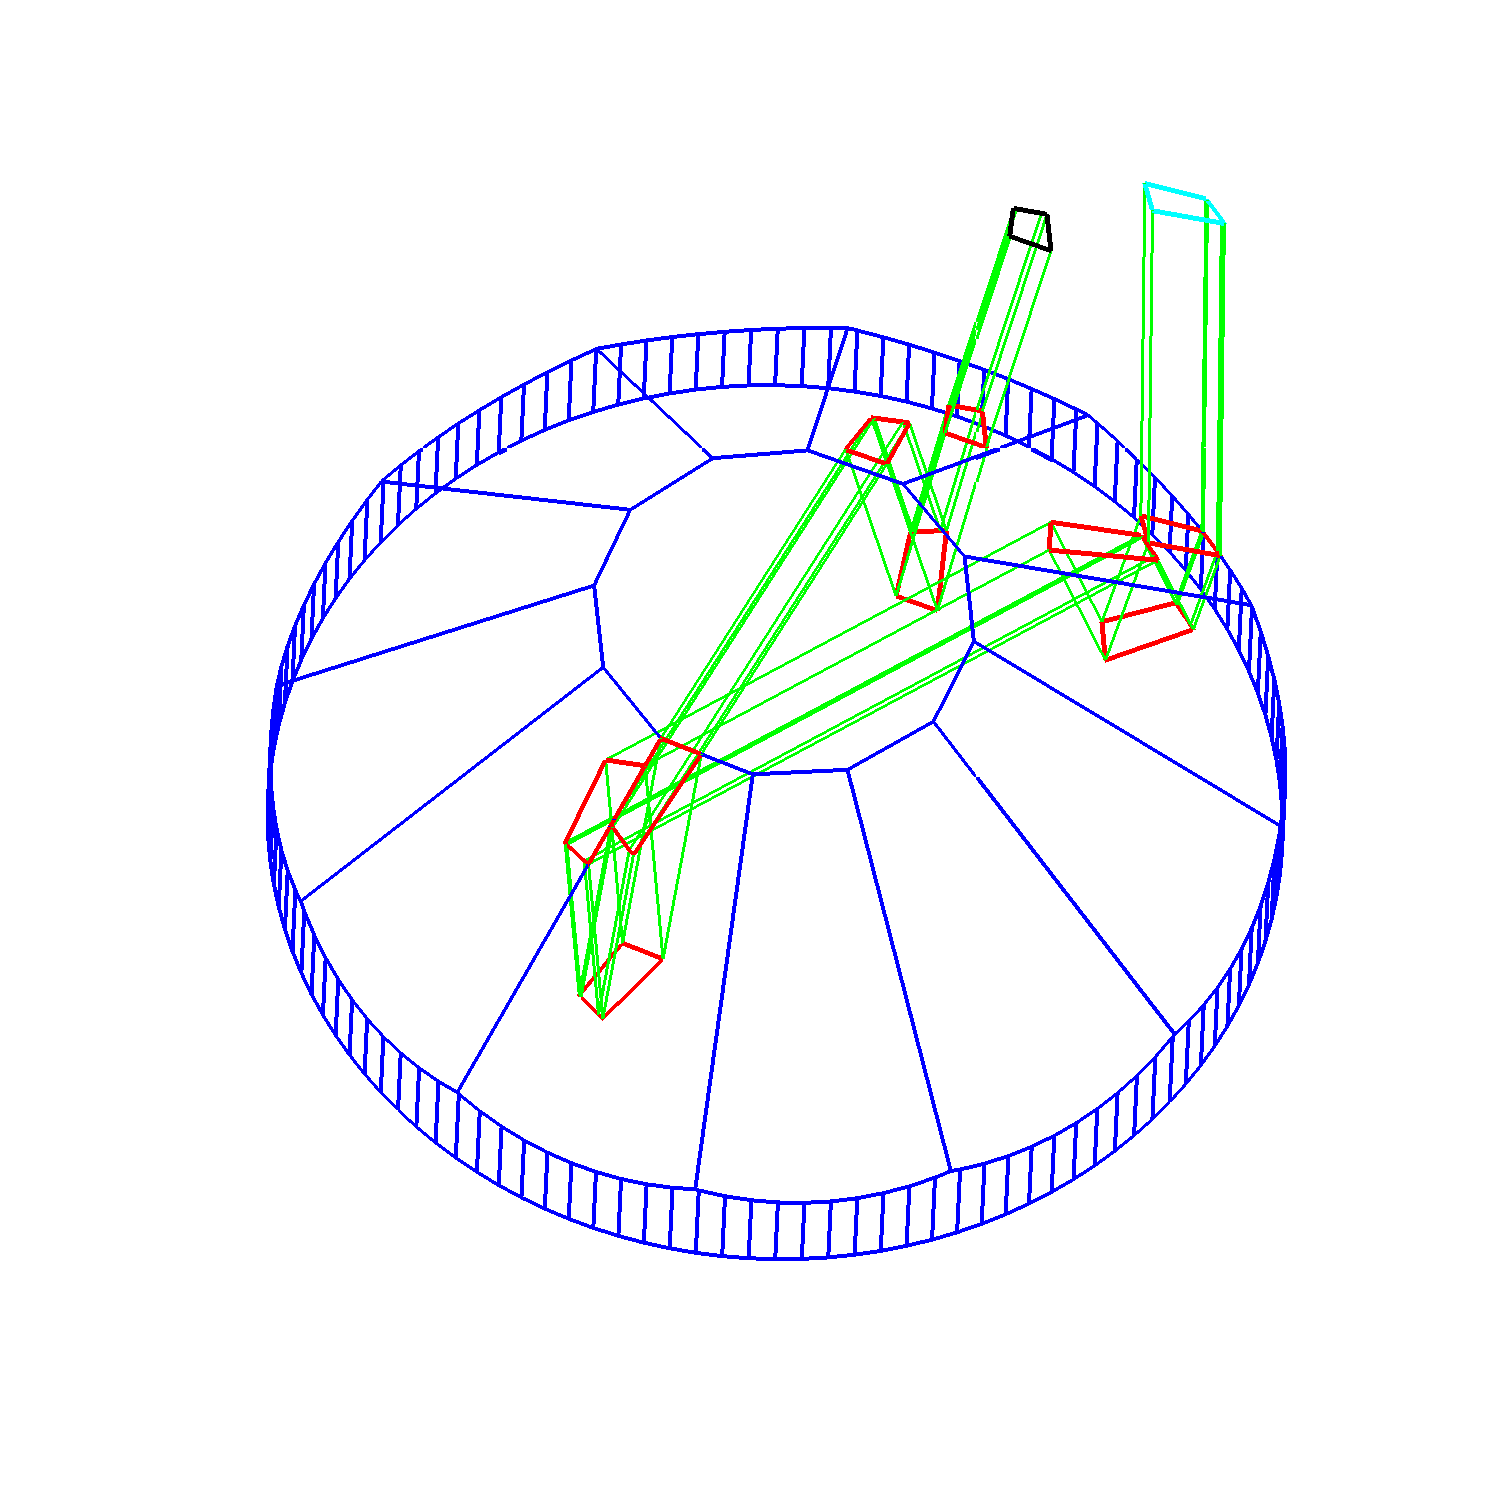
\includegraphics[width=\textwidth]{group9B.pdf}
\end{minipage}
\begin{minipage}[c]{0.325\textwidth}
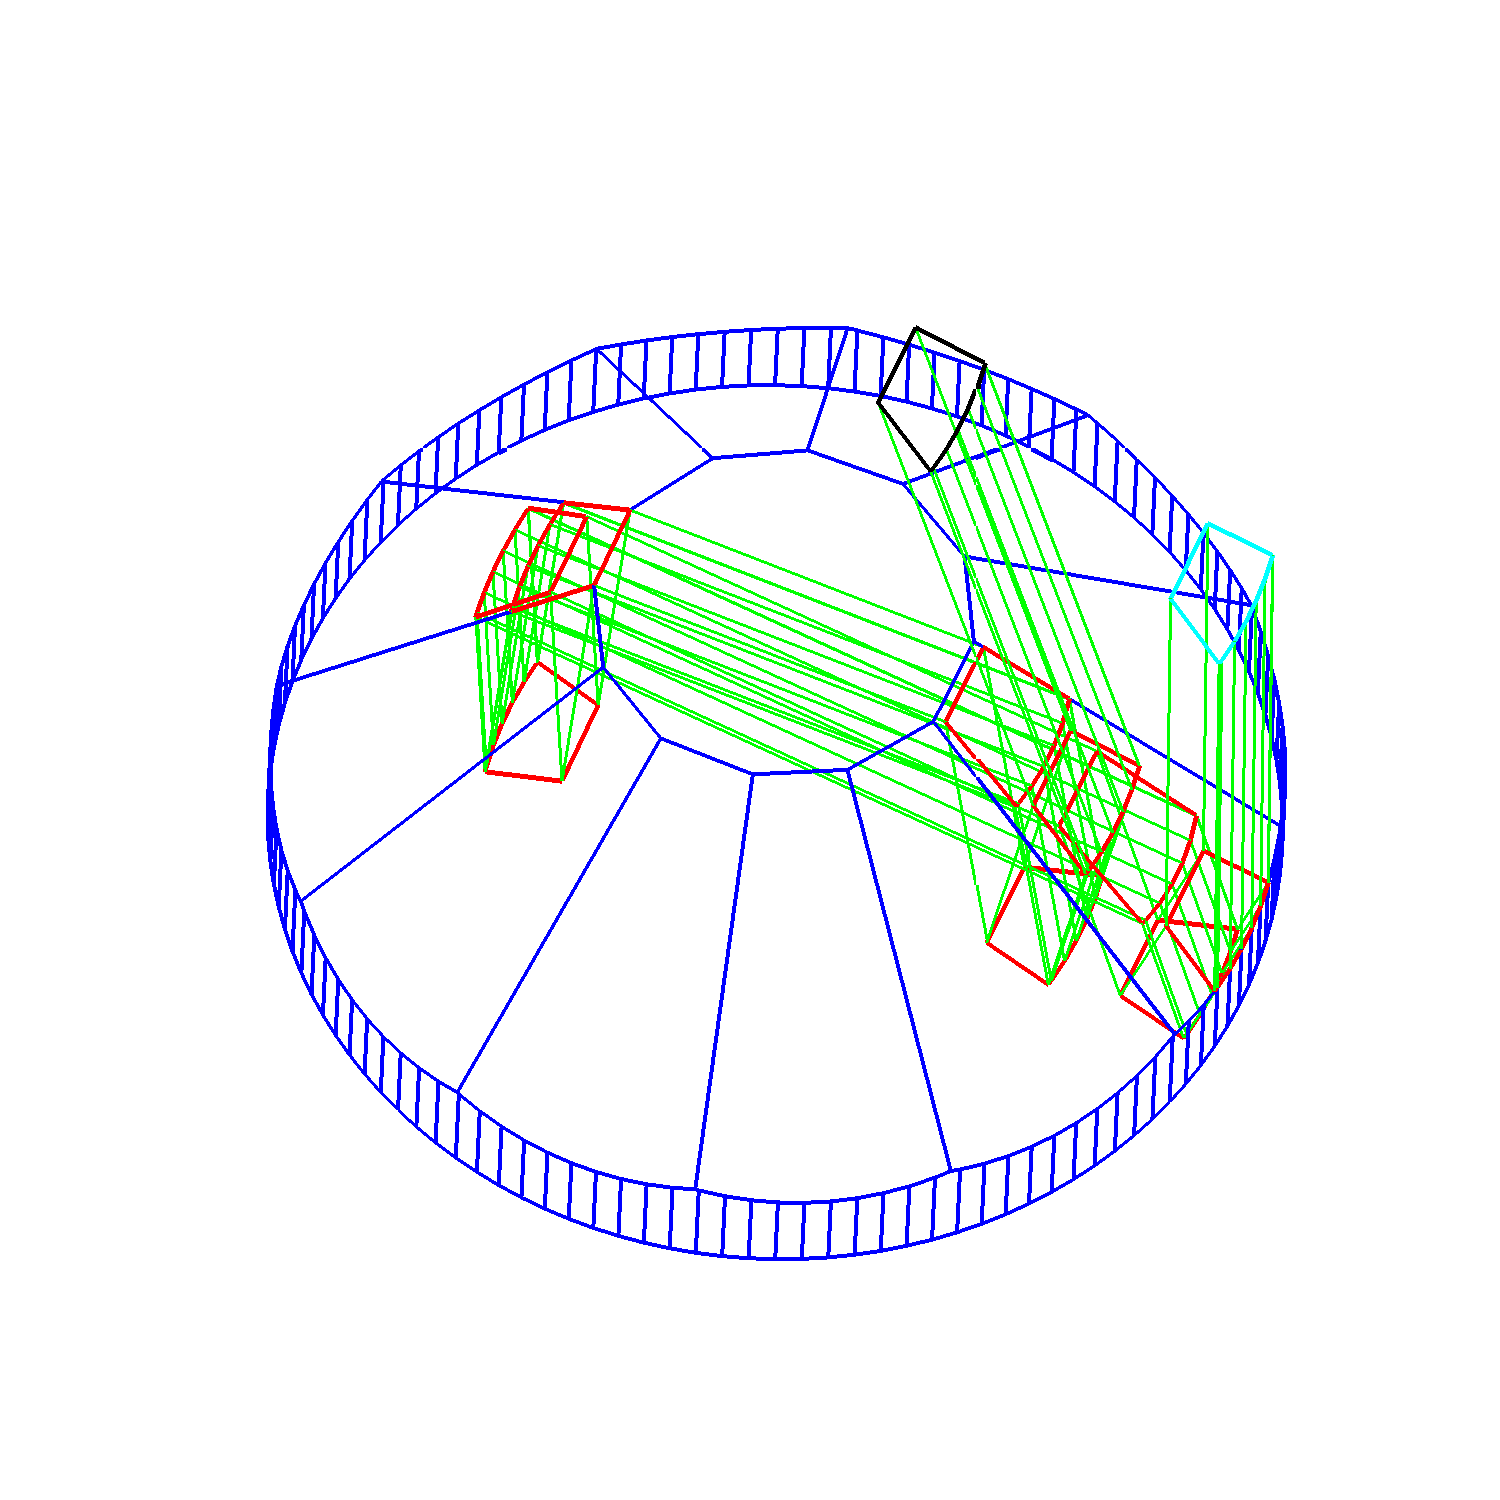
\includegraphics[width=\textwidth]{group9C.pdf}
\end{minipage}\\

\begin{minipage}[c]{0.325\textwidth}
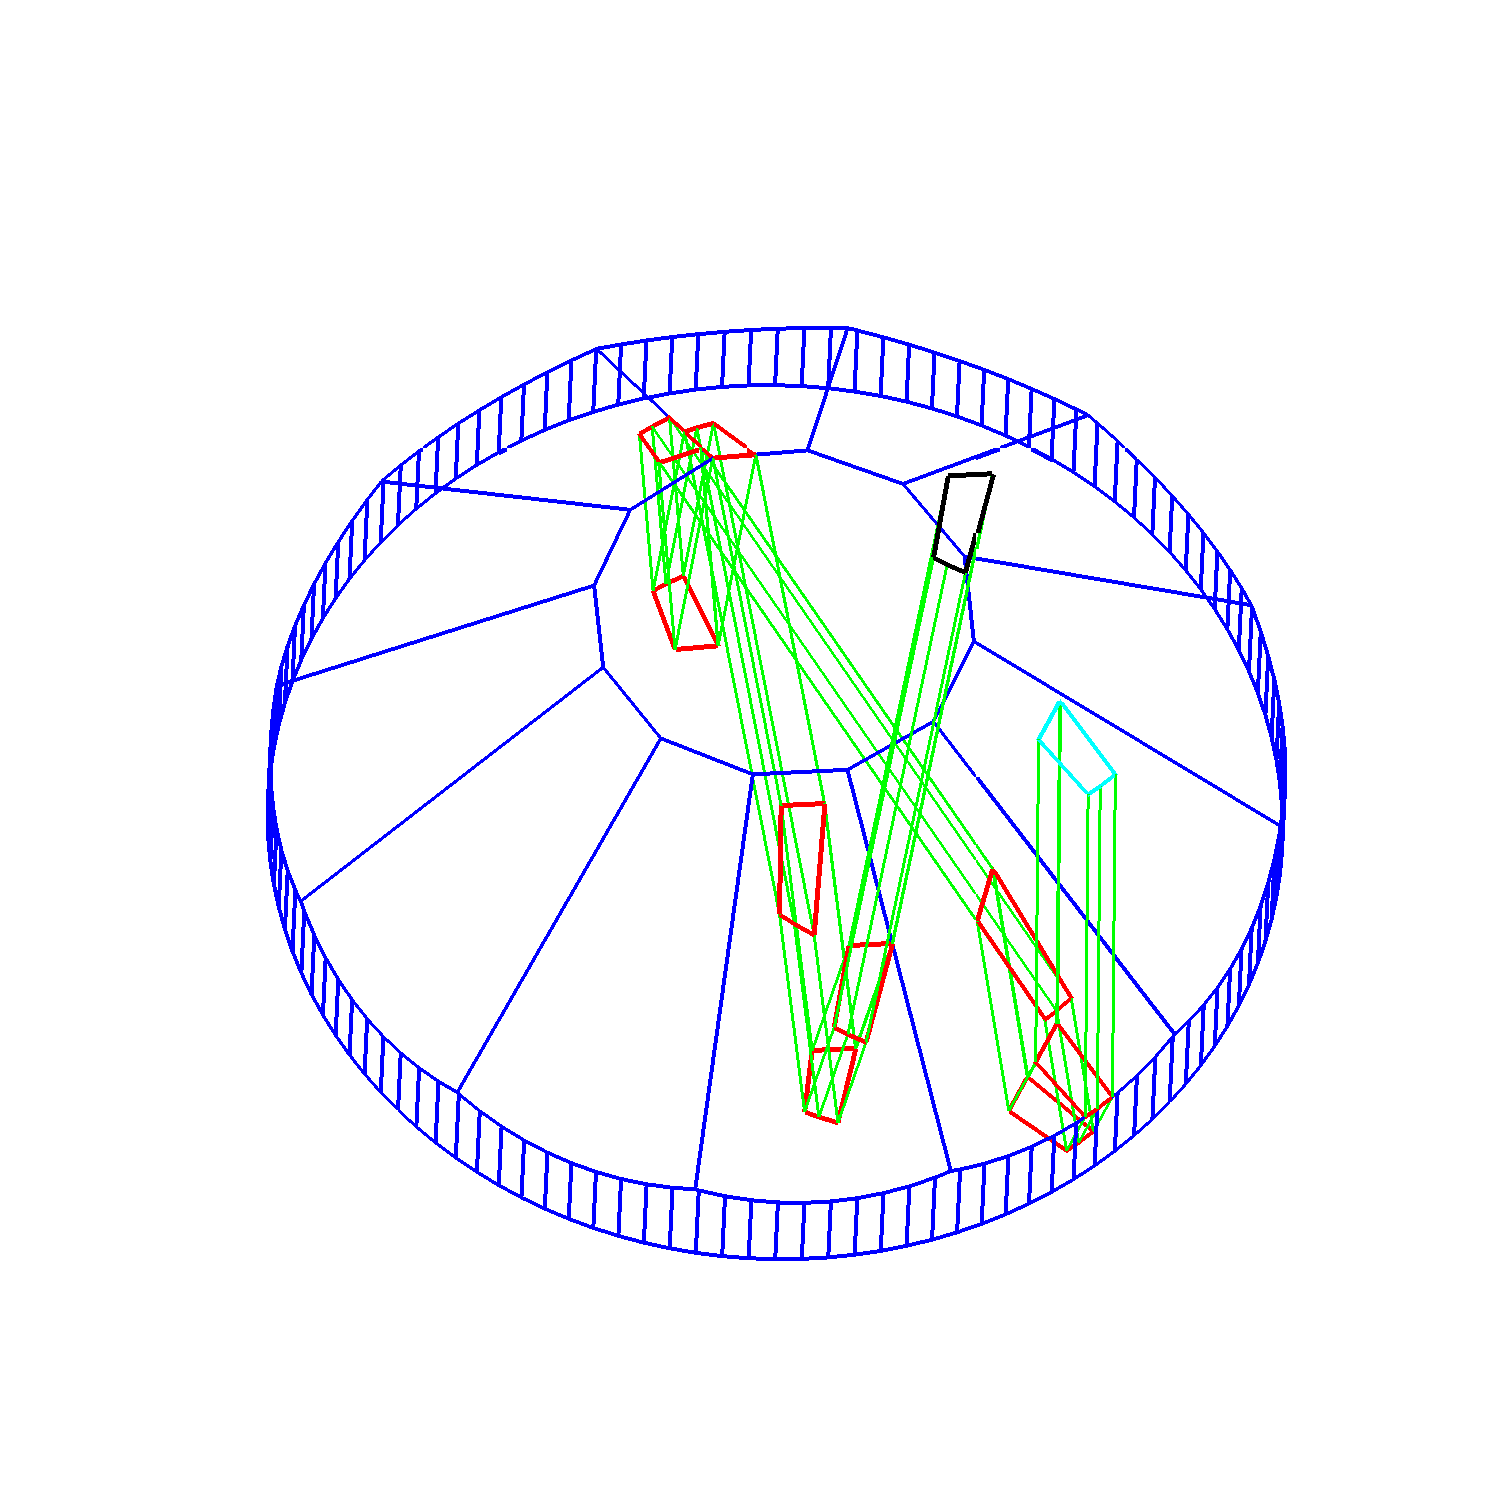
\includegraphics[width=\textwidth]{group9D.pdf}
\end{minipage}
\begin{minipage}[c]{0.325\textwidth}
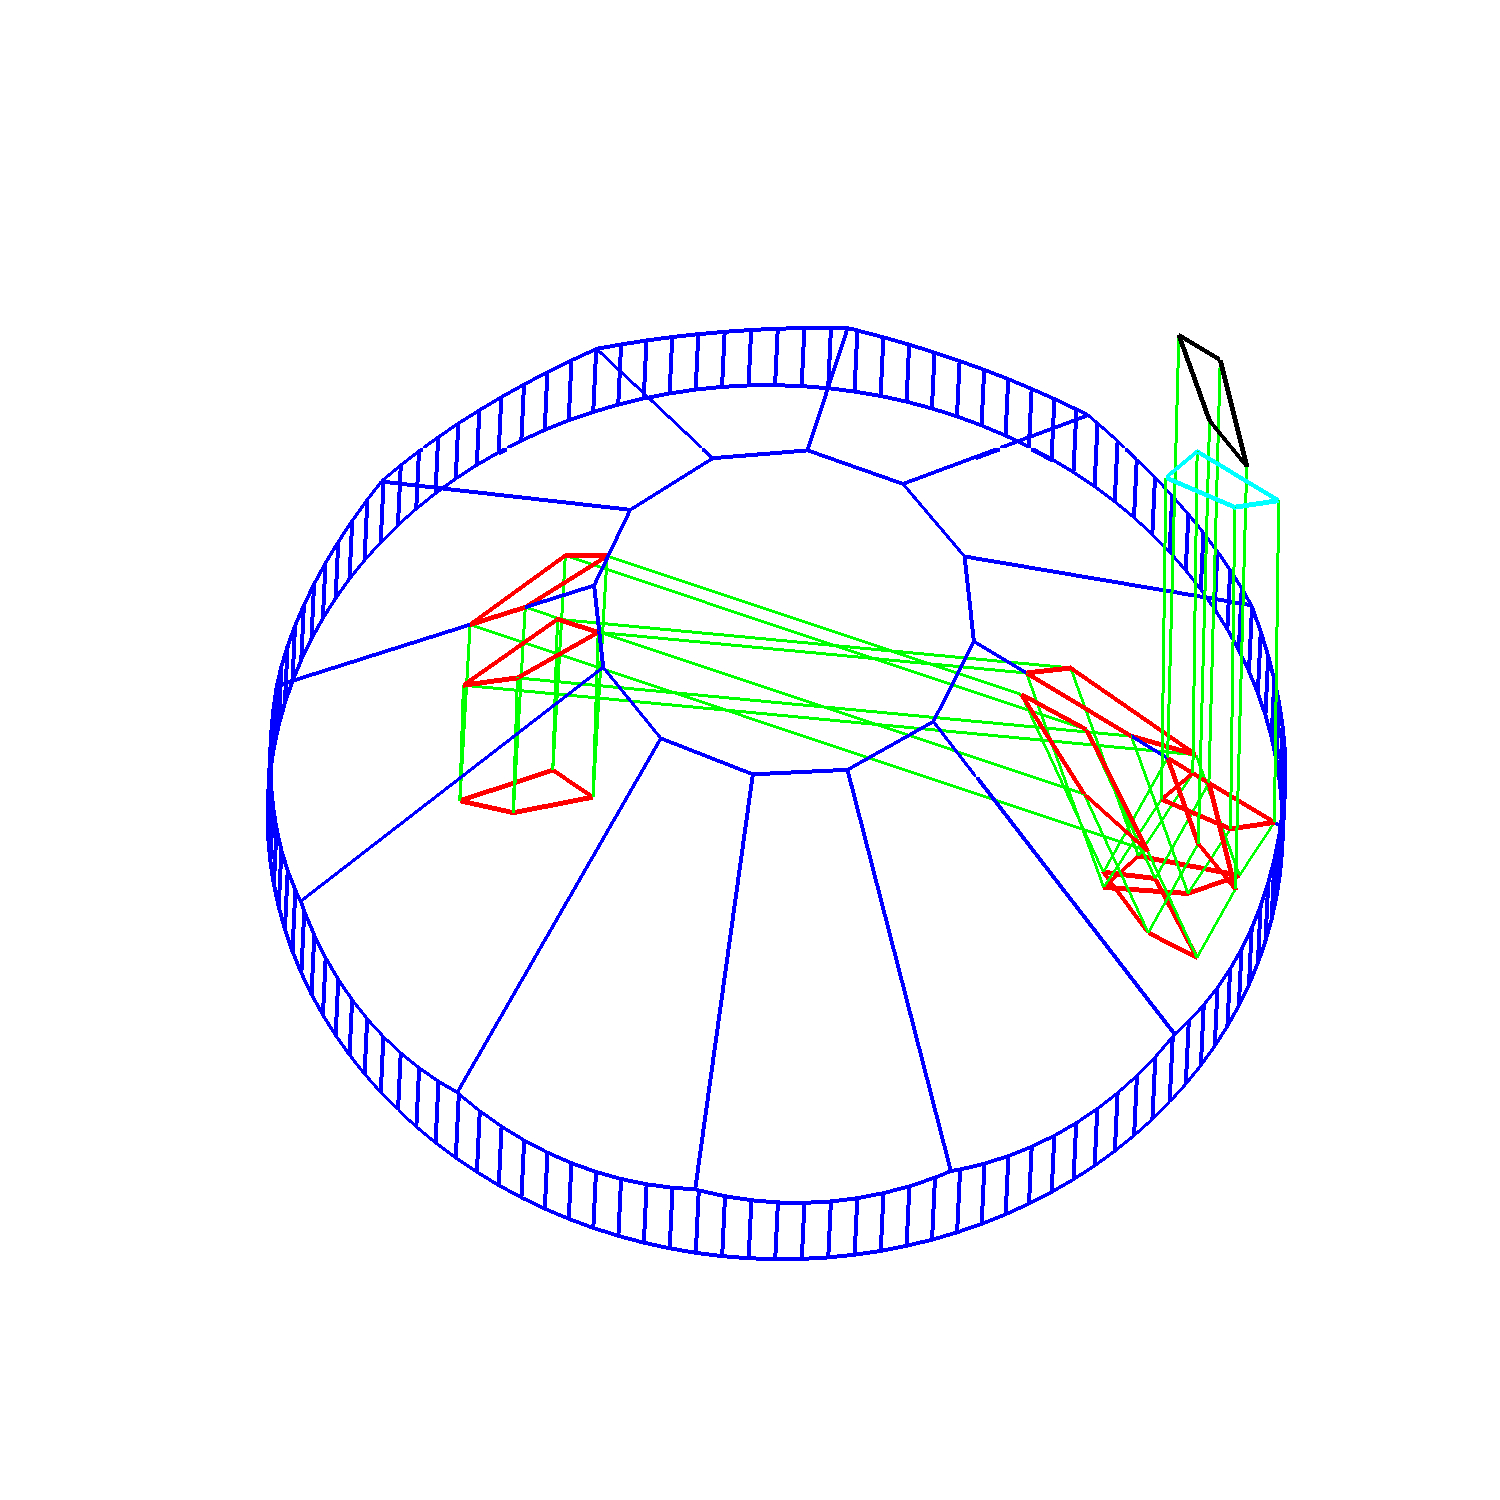
\includegraphics[width=\textwidth]{group9E.pdf}
\end{minipage}
\begin{minipage}[c]{0.325\textwidth}
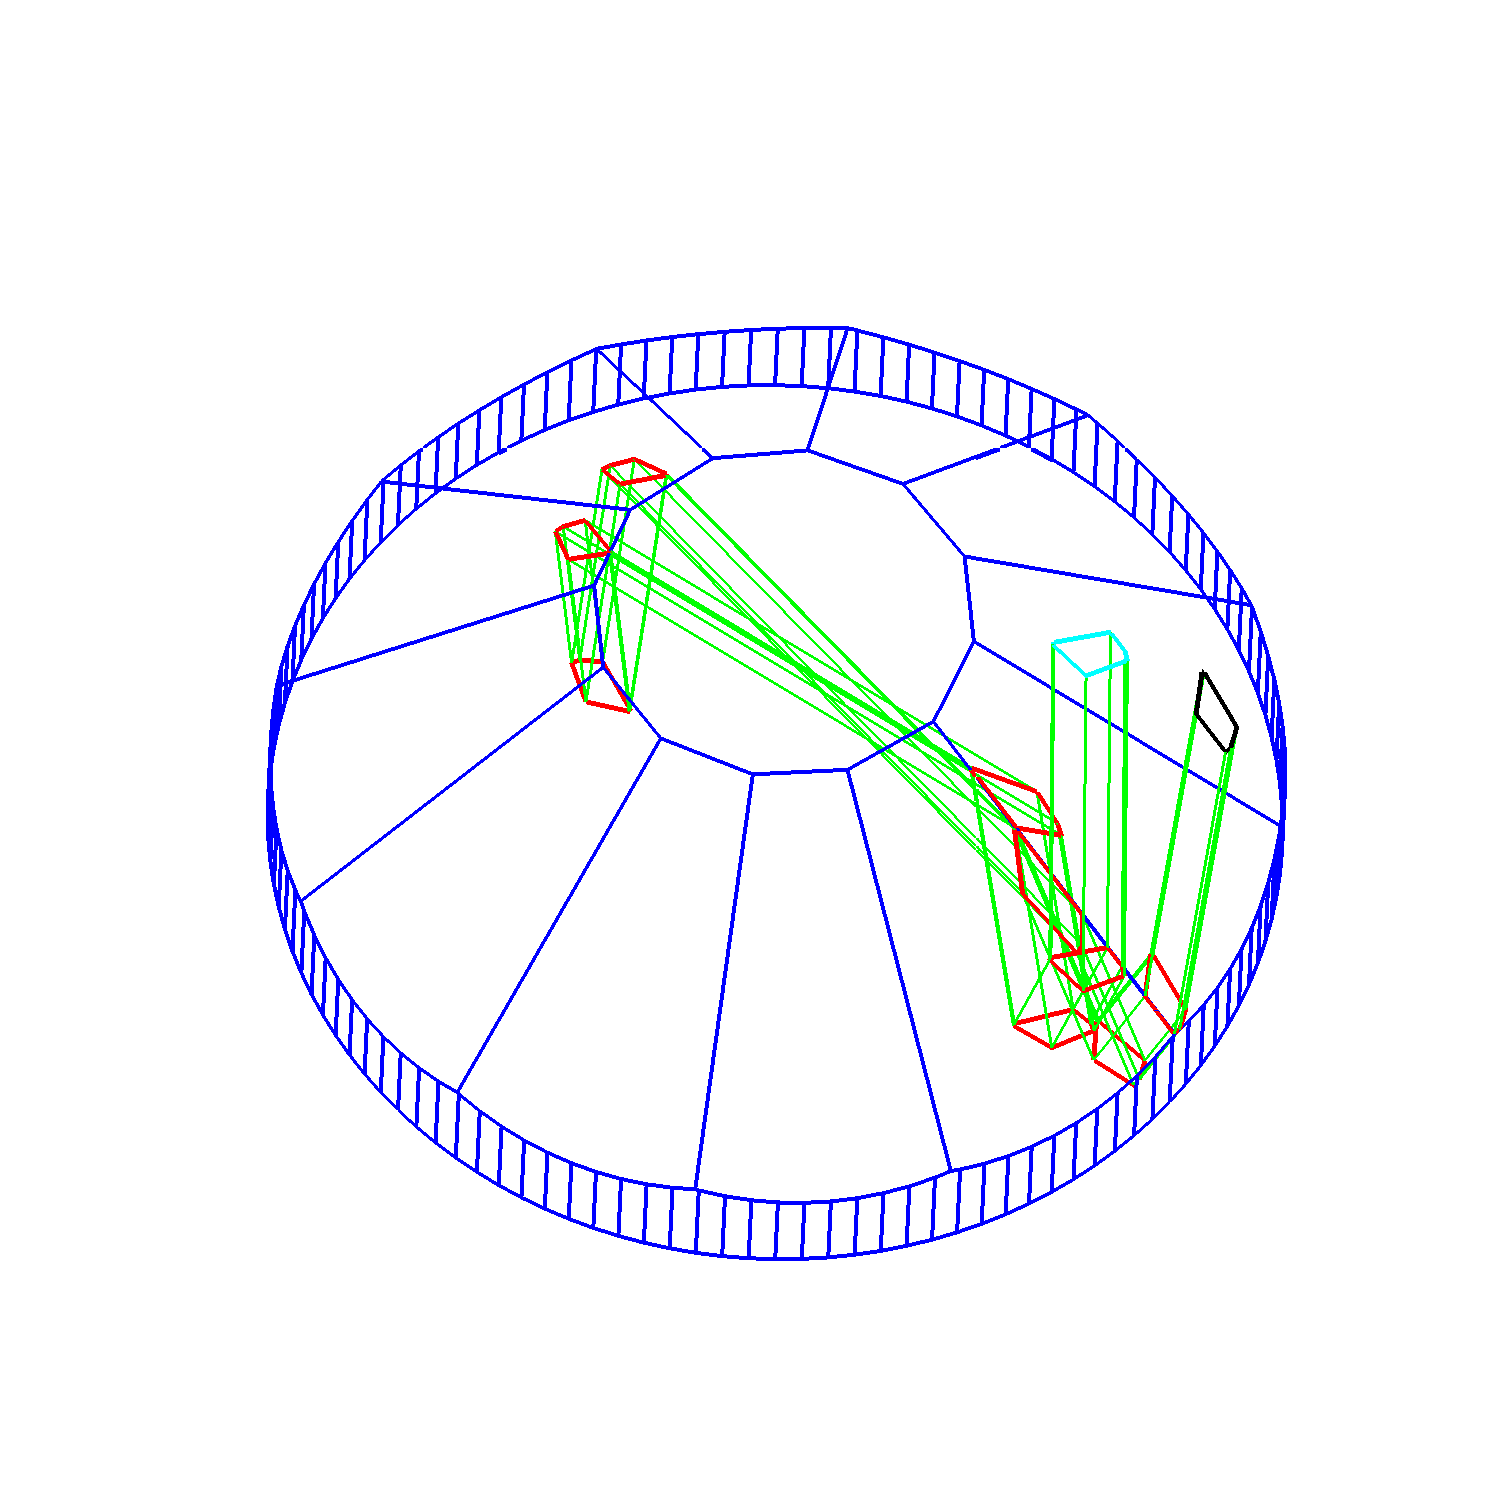
\includegraphics[width=\textwidth]{group9F.pdf}
\end{minipage}\\

\begin{minipage}[c]{0.325\textwidth}
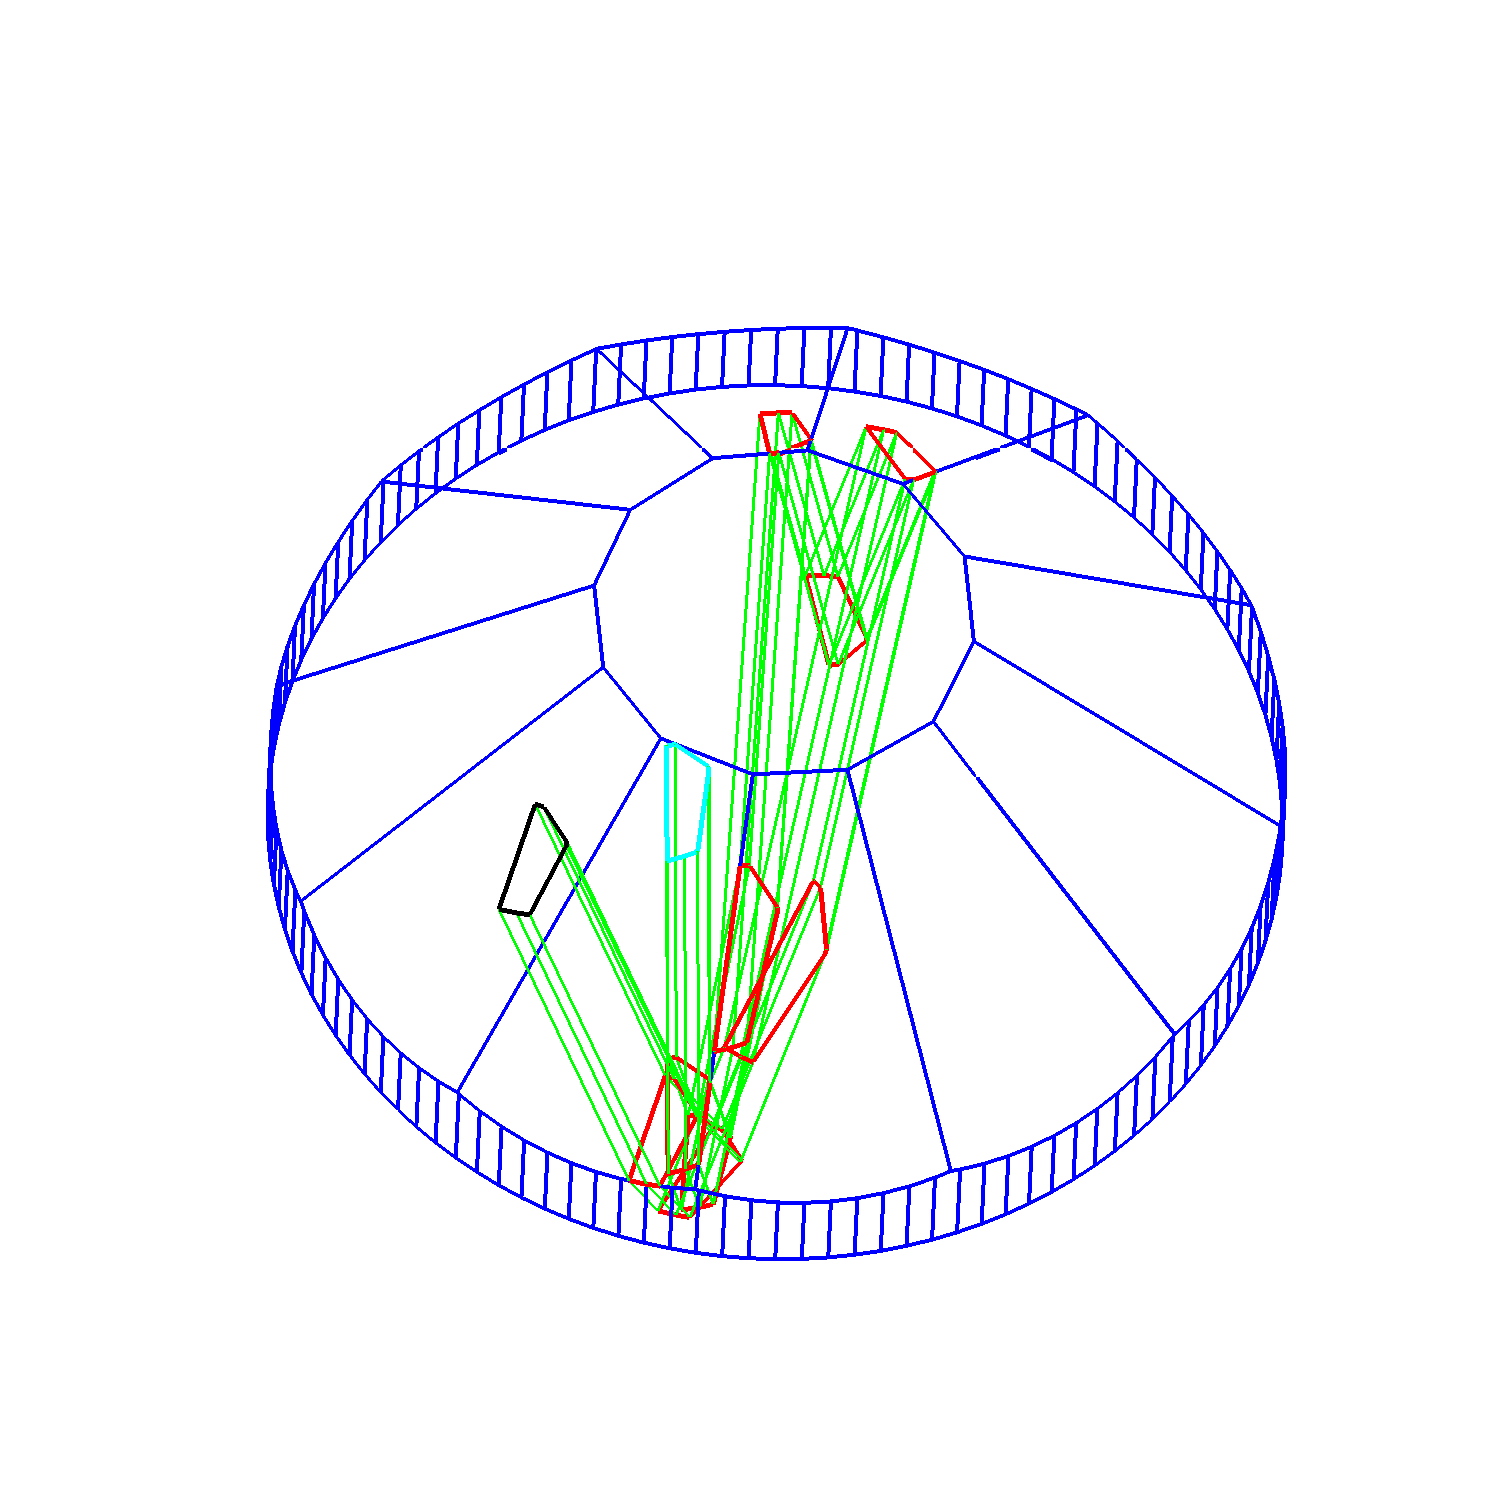
\includegraphics[width=\textwidth]{group9G.pdf}
\end{minipage}
\begin{minipage}[c]{0.325\textwidth}
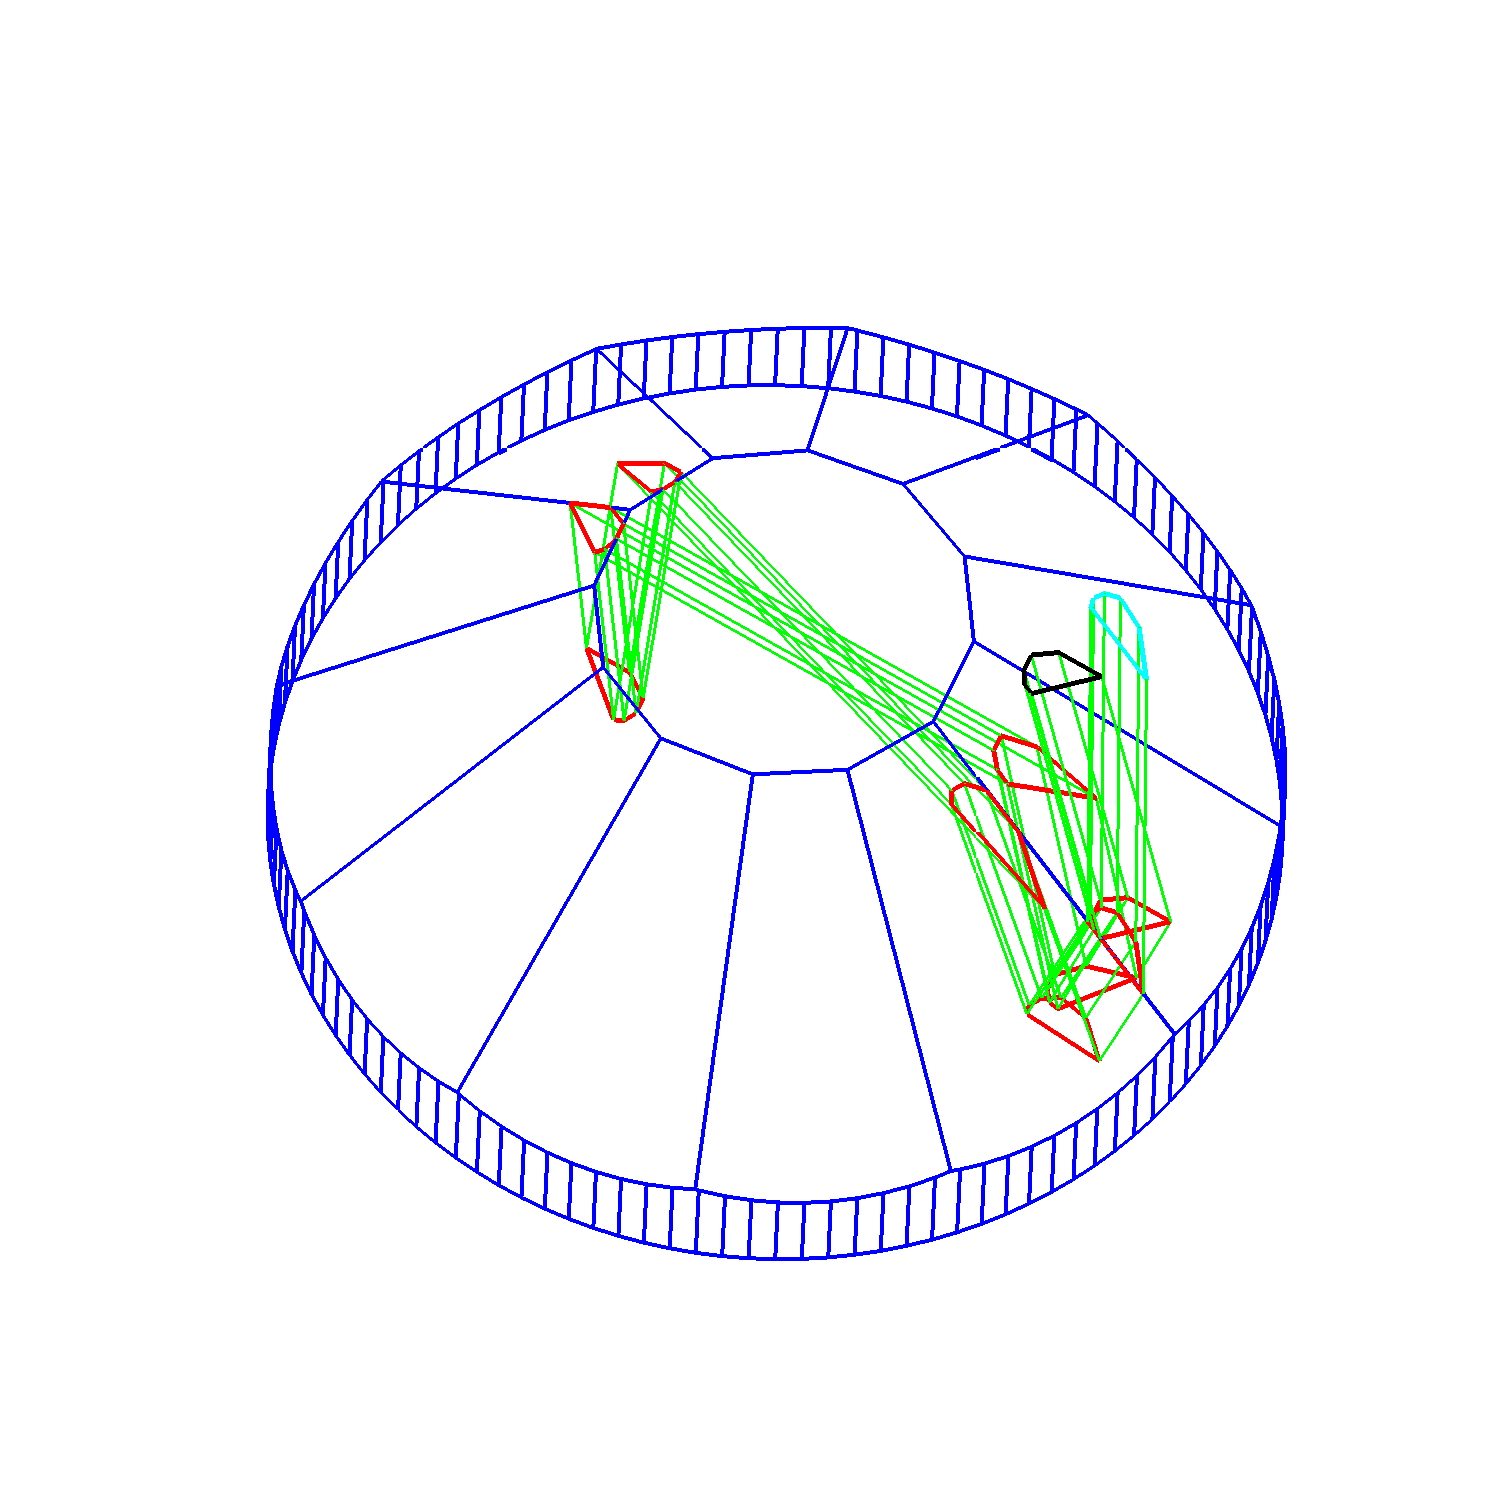
\includegraphics[width=\textwidth]{group9H.pdf}
\end{minipage}
\begin{minipage}[c]{0.325\textwidth}
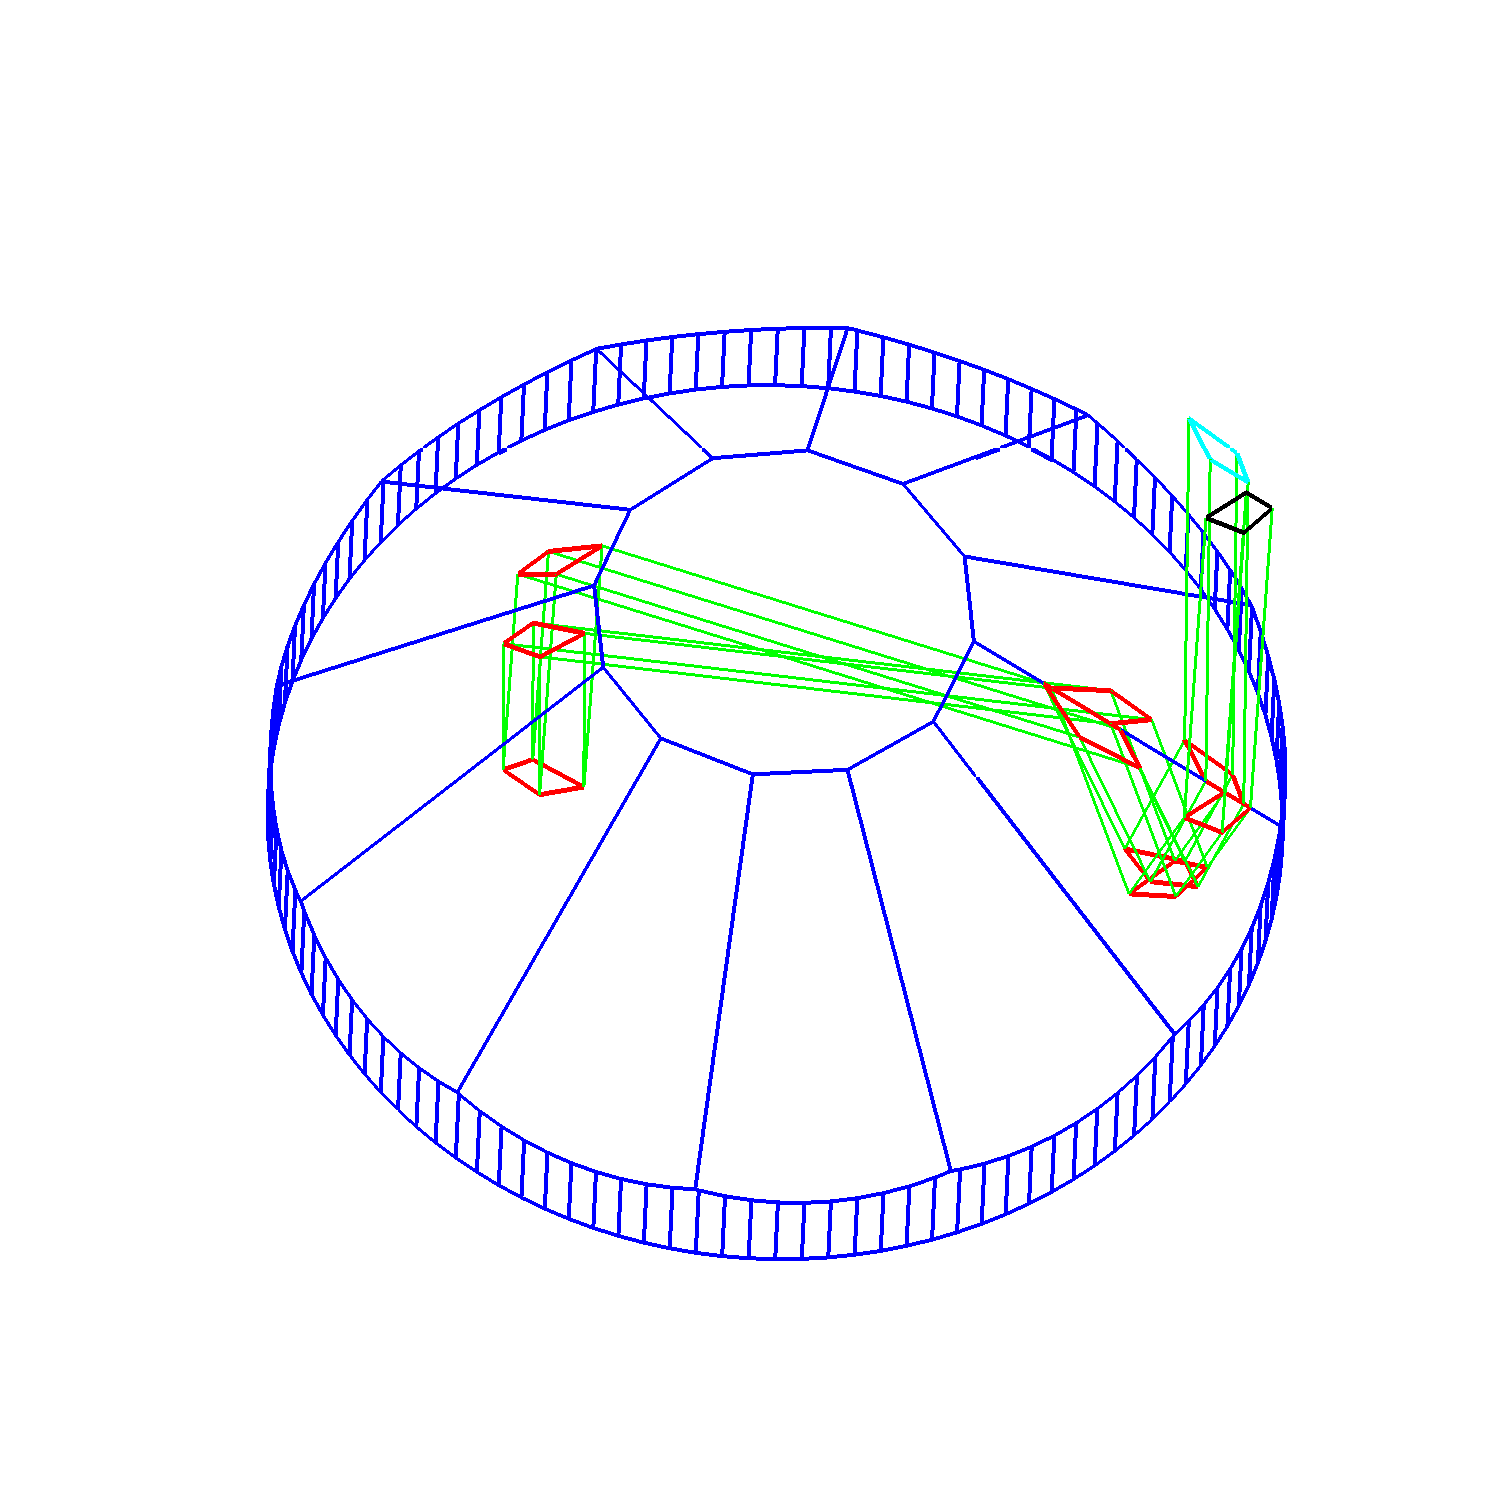
\includegraphics[width=\textwidth]{group9I.pdf}
\end{minipage}

\caption{3D view of ray example in classes 8B, 8C, 8D, 9A, 9B, 9C, 9D, 9E, 9F, 9G, 9H, 9I.}
\label{fig:modelClass3D1}
\end{figure}








